\documentclass[doktyp=marbeit, twoside]{TUBAFarbeiten}

\usepackage[ngerman,english]{babel}

\usepackage{selinput}% Auswahl der Dateikodierung (ansi,latin1,utf8,...)
	\SelectInputMappings{adieresis={ä},germandbls={ß},Euro={€}}% Zeichenzuordnung für selinput.sty
\usepackage[T1]{fontenc}% Einstellung Fontencoding

\usepackage{csquotes}% Einstellung zu Anführungszeichen; wird von biblatex.sty gefordert
\usepackage[backend=biber,style=authoryear-comp,sorting=nyt,sortlocale=de_DE_phonebook]{biblatex}% bessere Literaturverarbeitung
\addbibresource{literaturquellen.bib}

\usepackage[hidelinks]{hyperref}
\usepackage[table,figure]{hypcap}
\hyphenchar\font=\string"7F

\usepackage{tabularx,diagbox}
\usepackage{float}
\usepackage{multirow}
\usepackage{subcaption}

\usepackage{amsmath}
\usepackage{acronym}

\usepackage{listings}
\definecolor{gray}{rgb}{0.95,0.95,0.95}
\definecolor{violet}{rgb}{0.5, 0.0, 0.6}
\lstset{ basicstyle=\ttfamily\small, backgroundcolor=\color{gray} }
\lstset{ numbers=left, numberstyle=\tiny, numbersep=2pt }
\lstset{ breaklines=true, keywordstyle=\color{violet} }

%\usepackage{setspace}% Einstellungen Zeilenabstand
	%\onehalfspacing% Einstellungen Zeilenabstand

\setcounter{secnumdepth}{4}
% \setcounter{tocdepth}{4}

% Worttrennung für nicht bekannte Wörter
\hyphenation{Bei-spiel}
\hyphenation{TOTP}
\hyphenation{TOTPs}
\hyphenation{LimeSurvey}


\TUBAFFakultaet{Fakultät für Mathematik und Informatik}
\TUBAFInstitut{Institut für Informatik}
\TUBAFLehrstuhl{Professur für Ubiquitous Computing and Smart Systems}

%\TUBAFZweitlogo{\includegraphics{thekla_logo.jpg}}

\TUBAFTitel[Verbesserung der Benutzbarkeit und Sicherheit von Time-based One-time Passwords]{Verbesserung der Benutzbarkeit und Sicherheit gegen Man-In-The-Middle-Phishing von Time-based One-time Passwords}
\TUBAFBetreuer{\,Prof. \,Dr. Bastian Pfleging}
\TUBAFKorrektor{\,Prof. \,Dr. Florian Alt}
\TUBAFAutor[M. Käsemodel]{Marian Andreas Käsemodel}
\TUBAFStudiengang{Angewandte Informatik}
\TUBAFVertiefung{Technik}
\TUBAFMatrikel{62\,412}
\TUBAFDatum[]{\today}

\begin{document}

\maketitle

\TUBAFErklaerungsseite


\KOMAoptions{
	listof=totoc	% Abbildungs- und Tabellenverzeichnis im Inhaltsverzeichnis
}

\begin{abstract}
    \section*{Abstract}
Two-factor authentication is an effective protection against brute force or dictionary attacks. However, many of the current methods are neither user-friendly nor phishing-resistant. This paper presents a concept to make time-based one-time passwords more user-friendly and phishing-resistant. A study was conducted to evaluate how a prototype of the concept achieves these goals. It was found that the prototype is more user-friendly during authentication and only takes almost half as much time as the usual time-based one-time passwords.

\section*{Kurzzusammenfassung}
Zwei-Faktor-Authentisierung ist ein wirksamer Schutz gegen Brute-Force- oder Wörterbuchangriffe. Allerdings sind viele der gängigen Verfahren weder nutzerfreundlich noch Phishing-resistent. In dieser Arbeit wird ein Konzept vorgestellt, um Time-based One-time Passwords nutzerfreundlicher und Phishing-resistent zu machen. Mithilfe einer Studie wurde evaluiert, wie ein Prototyp des Konzepts diese Ziele erreicht. Es wurde festgestellt, dass der Prototyp bei der Authentisierung nutzerfreundlicher ist und nur fast nur halb so viel Zeit wie die gewöhnlichen Time-based One-time Passwords benötigt.
\end{abstract}
\newpage

\tableofcontents
\newpage
\section*{Abkürzungsverzeichnis}
\addcontentsline{toc}{section}{Abkürzungsverzeichnis}
\begin{acronym}
    \acro{2FA}{Zwei-Faktor-Authentisierung}
    \acro{API}{Application Programming Interface}
    \acro{APK}{Android Package Kit}
    \acro{BLE}{Bluetooth Low Energy}
    \acro{GSM}{Global System for Mobile Communications}
    \acro{HOTP}{HMAC-based One-time Password}
    \acro{HTML}{Hypertext Markup Language}
    \acro{LTE}{Long-term Evolution}
    \acro{MITM}{Man-In-The-Middle}
    \acro{MFA}{Multi-Faktor-Authentisierung}
    \acro{NFC}{Near Field Communication}
    \acro{OTP}{One-time Password}
    \acro{SEQ}{Single Ease Question}
    \acro{SIG}{Bluetooth Special Interest Group}
    \acro{SIM}{Subscriber Identity Module}
    \acro{SMS}{Short Message Service}
    \acro{SUS}{System Usability Scale}
    \acro{TOTP}{Time-based One-time Password}
    \acro{U2F}{Universal 2nd Factor}
    \acro{UEQ}{User Experience Questionnaire}
    \acro{USB}{Universal Serial Bus}
\end{acronym}
\newpage
\listoffigures
\newpage
\listoftables

\newpage
\section{Einführung}
	\label{sec: einfuhrung}

	\subsection{Problemstellung}
		\label{sec: problemstellung}
        Oft besitzen Personen schwache Passwörter oder verwenden das gleiche 
Passwort für mehrere Dienste, da sich so die Zugangsdaten einfacher merken 
lassen \autocite{PwReuse}. Daraus folgt, dass es Angreifern gelingt, mit 
Brute-Force-Methoden schwache Passwörter zu erraten oder mit gestohlenen 
Zugangsdaten eines Dienstes auch bei anderen Diensten Zugang zu erhalten.
\\\\
Da es nicht leicht ist, Nutzer zu einem anderen Verhalten zu bewegen und um 
mehr Sicherheit zu gewährleisten, bieten viele Dienste die 
Zwei-Faktor-Authentisierung (2FA) an. D.h. der Nutzer bestätigt seine 
Identität mit Benutzername und Passwort (erster Faktor) sowie mit einem 
zweiten Faktor, z.B. eine sechsstellige Zahl, die von einer Smartphone-App 
generiert wird. Allerdings stellt die Zwei-Faktor-Authentisierung einen 
zusätzlichen Aufwand für den Nutzer dar. 2FA kostet den Nutzer Zeit und 
lenkt ihn von der eigentlichen Aufgabe ab, die er erledigen möchte. Durch 
diese Unbequemlichkeiten ist die 2FA nicht attraktiv genug, dass Nutzer sie 
bei vielen Diensten verwenden. Meist nutzt man es nur bei Zugängen, die man 
als wichtig ansieht, oder weil man durch den Anbieter eines Dienstes dazu 
gezwungen wird.
\\\\
Außerdem haben die meisten gängigen 2FA-Verfahren eine Schwachstelle: sie 
sind nicht resistent gegen Phishing-Websites. Also Websites, die sich als 
eine originale Website ausgeben, ohne dass es der Nutzer bemerkt. In 
Echtzeit übertragen diese Websites die Nutzereingaben an die originale 
Website und imitieren perfekt die originale Website. Je nach 2FA-Verfahren 
gibt es noch mehr Schwachstellen oder einschränkende Bedingungen, wie eine 
vorausgesetzte Verbindung zum Internet.
\\\\
Seit ca. 2019 wurde eine neue Technologie namens Passkeys veröffentlicht. Sie 
basieren auf asymmetrischer Kryptographie und ermöglichen eine Anmeldung bei 
Online-Diensten ganz ohne Passwort und zweiten Faktor. Allerdings sind sie noch 
wenig verbreitet und es werden immer noch 
Phishing-anfällige sowie geringfügig nutzerfreundliche 2FA-Verfahren verwendet. 
Daher ist es sinnvoll, im Bereich der 2FA weiterhin zu forschen.

    \subsection{Ziel der Arbeit}
        \label{sec: ziel der arbeit}
        Ziel dieser Arbeit ist die Erweiterung des 2FA-Verfahrens der Time-based One-time 
Passwords (TOTP). Dadurch sollen TOTPs in der Nutzung  nutzerfreundlicher, 
zeiteffizienter und Phishing-resistent werden. Zunächst wird analysiert, welche 
Stärken das Verfahren aufweist und wieso es für eine Erweiterung geeignet ist. Dann 
werden die Schwächen bzgl. der Nutzerfreundlichkeit und des Phishing beleuchtet und 
Lösungen präsentiert. Dies vereint sich in einem Konzept, das anschließend mit 
einem Prototyp realisiert werden soll, um zu beweisen, dass das Konzept umsetzbar 
ist. Mithilfe einer Nutzerstudie wird das System hinsichtlich seiner 
Nutzerfreundlichkeit, Nutzererfahrung und Task Completion Time untersucht. Somit 
soll die Arbeit eine Antwort darauf geben, ob der neue Prototyp der TOTPs das 
Potential zu einer bedeutsamen Verbesserung bietet. Ziel der Arbeit ist es nicht, 
diesen Prototyp als marktfähiges Produkt zu entwickeln.

    \subsection{Aufbau der Arbeit}
        \label{sec: aufbau der arbeit}
        Zu Beginn der Arbeit wird ein Überblick über die 
Zwei-Faktor-Authentisierung, deren gängige Verfahren sowie 
weiterführende Technologien gegeben. Dann wird ein Konzept zur 
Verbesserung von Time-based One-time Passwords für mehr 
Benutzbarkeit und Schutz gegen Phishing vorgestellt. Dabei wird 
auch der Forschungsansatz mit seinen Forschungsfragen und 
Hypothesen definiert. Danach wird mit der Implementierung des 
vorgestellten Konzepts in Form eines Prototyps fortgefahren. 
Anschließend wird die Studie vorgestellt, die der Untersuchung 
des Prototyps bezüglich seiner Nutzerfreundlichkeit, 
Nutzererfahrung und Task Completion Time dient. Am Ende werden 
die Studienergebnisse präsentiert, diskutiert und ein Ausblick 
gegeben.

\newpage
\section{Grundlagen und verwandte Arbeiten}
    \label{sec: grundlagen}
    Zunächst werden einige Grundlagen bzgl. der Zwei-Faktor-Authentisierung  geklärt. 
Dabei werden gängige Verfahren sowie deren Stärken und Schwächen bzgl. der Sicherheit 
und Nutzerfreundlichkeit betrachtet. Es wird die Problematik des Phishings vorgestellt 
und anschließend Passkeys sowie verwandte Arbeiten besprochen. 

    \subsection{Zwei-Faktor-Authentisierung}
        \label{sec: 2fa}
        Zwei-Faktor-Authentisierung (2FA), auch Zwei-Faktor-Authentifizierung genannt, ist 
der Nachweis bzw.\ die Prüfung einer Identität über zwei verschiedene Faktoren. Es 
gibt drei Arten von Faktoren: das Wissen über eine Information (etwas, das man 
weiß), der Besitz eines Gegenstands (etwas, das man hat), und die Inhärenz einer 
nicht übertragbaren Eigenschaft des Individuums (etwas, das man ist) \autocite[2]{Marky}. 
Authentisierung bedeutet also das Erbringen eines Nachweises für die Identität, 
während die Authentifizierung die Prüfung dieses Nachweises meint.
\\\\
\textit{\textbf{Konvention}}:
Es gibt keinen allgemeinen Oberbegriff für die beiden Begriffe \glqq Authentisierung\grqq{} und \glqq Authentifizierung\grqq{}, daher wird in dieser Arbeit der 
Begriff \glqq Authentisierung\grqq{} stellvertretend als Oberbegriff verwendet. Denn 
letztlich fokussiert sich diese Arbeit auf die Art und Weise, wie sich eine Partei authentisiert (ausweist). Die Abläufe der Authentifizierung sind zweitrangig.
\\\\
Das Wissen über eine Information ist bspw.\ ein Passwort. Jeder, der das Passwort 
kennt, kann die Identität des zugehörigen Benutzernamen bezeugen. Jedoch sind 
Passwörter oft zu schwach und können erraten werden. Das kann auch automatisiert 
geschehen, indem bspw.\ mit Brute-Force- oder Dictionary-Attacken versucht wird, das 
Passwort zu erraten \autocite[1162 \psqq]{Bosnjak}.
\\\\
Der Besitz eines Gegenstands kann auch die Identität bezeugen. Beispiele für 
solche Gegenstände sind physische Token (USB-Hardware), Smartcards, Kreditkarten 
oder das Smartphone \autocite[2]{Marky}. Problematisch ist hierbei der Verlust 
oder Diebstahl eines solchen Gegenstands.
\\\\
Die dritte Art von Faktoren beschreibt etwas, das man ist. Genauer gesagt etwas, das das Individuum eindeutig identifiziert. Beispiele sind biometrische Eigenschaften 
wie Fingerabdrücke oder Gesichtsmerkmale. \autocite[2]{Marky}
\\\\
Das Prinzip der 2FA sieht vor, dass die zwei Faktoren von verschiedener Art sind. Im 
Kontext bei Online-Accounts auf Webseiten oder Anwendungen ist ein Faktor meist das 
Passwort, also etwas, das man weiß und der zweite Faktor etwas, das man besitzt 
(meist das Smartphone oder physische Token). 2FA ist natürlich auch in anderen 
Kontexten vorgesehen wie bei Zugängen von Gebäuden oder Räumen. Hier könnte ein 
Faktor in Form von biometrischen Daten und ein Passwort üblich sein. Man nutzt 2FA, da es mehr Sicherheit bietet als nur einen Faktor zu verwenden, der im Fall von Passwörtern keinen ausreichenden Schutz bietet.
\\\\
Die 2FA ist eine Spezialisierung der Multi-Faktor-Authentisierung (MFA), die wiederum 
besagt, dass zwei oder mehr unabhängige Faktoren bei der Authentisierung verwendet 
werden.

    
    \subsection{Verfahren der Zwei-Faktor-Authentisierung}
        \label{sec: verfahren der 2fa}
        In diesem Kapitel werden die gängigen 2FA-Verfahren im Kontext von 
Online-Anwendungen vorgestellt. Des Weiteren werden auch die Vor- und Nachteile dieser Verfahren beleuchtet. 
Leider gibt es nur wenige Studien zu 2FA-Verfahren, die insbesondere verlässliche 
Zeitmessungen bzgl. der Nutzerinteraktionen bieten. Grundlegende Erkenntnisse liefert die Studie 
von \textcite{Reese}. Hier wurden verschiedene 
2FA-Verfahren hinsichtlich ihrer Nutzerfreundlichkeit und ihres Zeitaufwandes 
untersucht. Es wurden die gängigsten Verfahren untersucht:
\begin{itemize}
    \item Vorab generierte Codes
    \item Push-Benachrichtigungen (Authy)
    \item Einmalpasswort per SMS
    \item Zeitbasiertes Einmalpasswort (Google Authenticator)
    \item Universal Second Factor Security Keys (USB-Gerät YubiKey)
    \item Nur Passwort ohne zweiten Faktor (als Kontrollgruppe)
\end{itemize}
Dabei gab es sechs Studiengruppen mit je 12 Teilnehmern. Jede Studiengruppe hat eine 
der sechs untersuchten Authentisierungsverfahren eingerichtet und in einer 
zweiwöchigen Phase genutzt, um sich täglich bei einem Webdienst anzumelden. Es 
wurde die benötigte Zeit für die Einrichtung des Verfahrens sowie für die Eingabe bzw. 
Bestätigung des zweiten Faktors serverseitig gemessen. 
Neben qualitativen Ergebnissen aus Interviews wurde unter anderem auch die Benutzbarkeit mit der System 
Usability Scale (SUS) ermittelt.
\\\\
In der Studie gibt es pro Studiengruppe (also pro Verfahren) eine Zeitmessung und 
eine SUS-Bewertung für den Authentisierungsprozess. Die Ergebnisse sind in Abb. \ref{fig: reese sus} und Abb. \ref{fig: reese zeiten} dargestellt. Die zugehörigen Tabellen für die exakten Werte befinden sich im Anhang \ref{anh: reese}.
\\
\begin{figure}
    \begin{minipage}[b]{.48\textwidth}
        \centering
        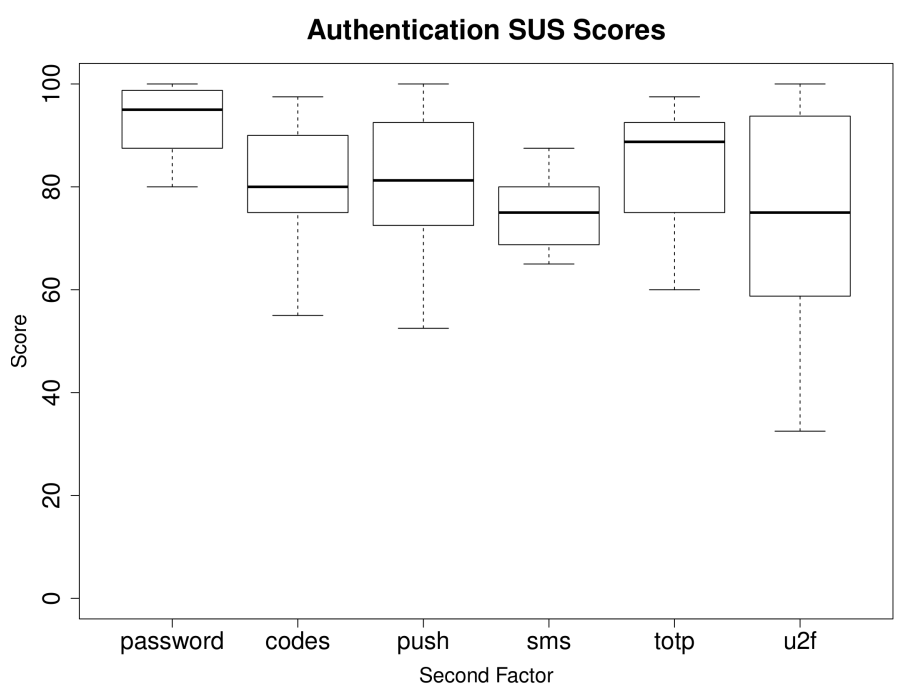
\includegraphics[width=1\linewidth]{figures/susAuth.png}
        \caption[SUS-Bewertung für die Authentisierung mit verschiedenen 2FA-Verfahren]{SUS-Bewertung für die Authentisierung mit verschiedenen 2FA-Verfahren, entnommen aus \autocite[363]{Reese}}
        \label{fig: reese sus}
    \end{minipage}
    \hfill
    \begin{minipage}[b]{.48\textwidth}
        \centering
        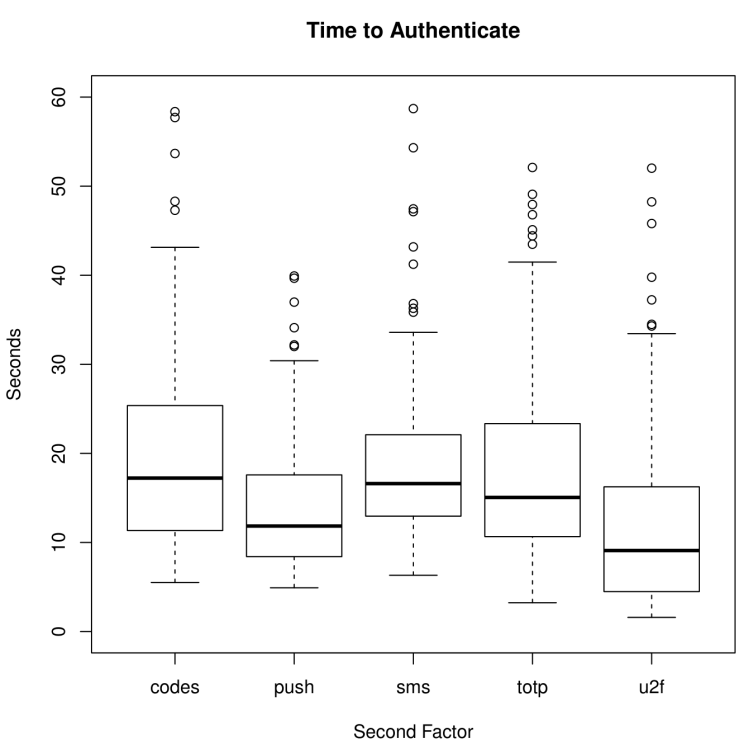
\includegraphics[width=1\linewidth]{figures/timeToAuth.png}
        \caption[Benötigte Zeit für die Authentisierung mit verschiedenen 2FA-Verfahren]{Benötigte Zeit für die Authentisierung mit verschiedenen 2FA-Verfahren, entnommen aus \autocite[362]{Reese}}
        \label{fig: reese zeiten}
    \end{minipage}
\end{figure}

Im Verlauf dieses Kapitels werden die Ergebnisse genutzt, um die vorgestellten 
2FA-Verfahren bzgl. ihrer Nutzerfreundlichkeit und ihres Zeitaufwandes einzuordnen.


        \subsubsection{Vorab generierte Codes}
        \label{sec: codes}
        Bei diesem Verfahren generiert der Dienstanbieter vorab einige Codes und lässt sie 
dem Nutzer zukommen (Email, Papierform, direkte Anzeige der Codes nach Einrichtung 
des Verfahrens). Diese Codes sind jeweils nur eine zufällige Zeichenabfolge, die im 
besten Fall nur einmal gültig ist. Bei der Anmeldung gibt der Nutzer nach Eingabe 
des Benutzernamens und des Passworts einen der Codes ein und ist erfolgreich 
angemeldet. Den verwendeten Code kann er dann verwerfen.
\\\\
Das Prinzip ist einfach aufgebaut (Code ablesen, eintippen und von der Liste streichen), aber es gibt einige Schwachstellen. Die Codes müssen  auf beiden 
Seiten sicher verwahrt sein. Der Anbieter kann die Codes sicher hashen, doch der 
Nutzer muss sie entweder in Papierform verwahren (im Klartext) oder in einer Datei 
(bestenfalls verschlüsselt) speichern. Außerdem sind die Codes so lange gültig, bis 
der Nutzer sie verwendet. D.h. mittels Brute-Force-Attacken, kann ein Angreifer den 
Code erraten. Aus diesem Grund sollten die Codes auch eine ausreichende Anzahl an 
Zeichen zählen. Das wiederum erfordert, dass der Nutzer bei der Eingabe des Codes 
viele Zeichen ablesen und eintippen muss. Dadurch steigt die Fehleranfälligkeit und 
der Zeitaufwand bei der Eingabe. Außerdem besteht ein Problem, wenn der Nutzer die 
Codes verliert bzw. versehentlich löscht, ohne Sicherheitskopien angelegt zu haben. \autocite[359 \psq]{Reese}
\\\\
Nach der Studie von \textcite{Reese} haben die generierten Codes bei der 
Authentisierung (nicht der Einrichtung) einen Medianwert von 80 und einen 
arithmetischen Mittelwert von $80{,}2$ in der SUS-Bewertung. Somit 
liegen sie im Vergleich zu den anderen untersuchten 2FA-Verfahren im mittleren 
Bereich. Zeitlich haben sie den größten Aufwand mit einem Median von $17{,}2~s$ und einem 
arithmetischen Mittelwert von $28~s$. Ob die Teilnehmer ihr 
benötigtes Mittel (hier die Codes) für den Zweiten-Faktor-Schritt bereits vor der 
Anmeldung bereitliegen hatten, wurde in der Studie nicht unterschieden. D.h. bei den 
gemessenen Zeiten ist stets unklar, ob und wie viel Zeit für das Beschaffen des 
Mittels benötigt wurde \autocite[364]{Reese}. Auch wurde nicht erwähnt, wie viele Zeichen jeder 
Code enthält.


        \subsubsection{Einmalpasswörter über SMS}
        \label{sec: sms}
        Ein bekanntes Verfahren sind Einmalpasswörter (meist sechsstellige Zahlen), die nach 
Eingabe von Nutzername und Passwort per SMS an das Smartphone des Nutzers gesendet 
werden. Auch die Übertragung des Einmalpassworts per E-Mail ist üblich, soll hier 
aber nicht näher betrachtet werden. Bzgl. der Nutzerfreundlichkeit teilen SMS und 
E-Mail sich einige Eigenschaften. Der Nutzer liest den empfangenen Code ab und gibt 
ihn dann auf der Login-Seite ein. Nach der Verwendung verliert das Einmalpasswort 
seine Gültigkeit. Diese sollte im Idealfall nur für wenige Minuten gültig sein.
\\\\
Die Methode wird oft genutzt und hat wie die anderen smartphone-basierten Verfahren 
den Vorteil, dass kein extra Gegenstand benötigt wird. Jedoch hat das SMS-Verfahren 
ähnliche Kritikpunkte wie die generierten Codes. Auch hier muss der Code abgelesen 
und eingetippt werden, wobei Zeichen fehlerhaft übernommen werden könnten. Außerdem 
ist auch hier der Verlust des Geräts ein Problem. Dafür könnte man die vorab 
generierten Codes als Backup-Lösung nutzen, sofern der Dienst dies unterstützt. Aber 
auch dies öffnet, wie bereits erwähnt, Angriffsmöglichkeiten.
\\\\
Ein weiteres Problem ist das SIM-Swapping. Hierbei kontaktiert der Angreifer den 
Kundenservice des Mobilfunkanbieters des Nutzers. Mit einem plausiblen Grund (z.B. 
Verlust des Smartphones) gelingt es dem Angreifer, den Mobilfunk-Account des Nutzers 
einer neuen SIM-Karte zuzuweisen, die ihm der Mobilfunkanbieter dann zusendet. Von 
nun an empfängt der Angreifer die SMS-Nachrichten, die eigentlich an den Nutzer 
gerichtet sind. \autocite[51 \psq]{Jover}
\\\\
Jovers Zusammenfassung zufolge gibt es in den Netzwerken des Global System for 
Mobile Communications (GSM) sowie Long-term Evolution (LTE) Schwachstellen, die es 
dem Angreifer ebenfalls ermöglichen, den SMS-Verkehr des Nutzers auf das Gerät des 
Angreifers umzuleiten. Voraussetzung sei, dass der Angreifer Zugriff auf einen 
Entry-Point des \glqq Signaling System 7\grqq{}-Netzwerks benötigt. \autocite[51]{Jover}
\\\\
Auch der später in Kap. \ref{sec: phishing} (S. \pageref{sec: phishing}) beschriebene Phishing-Angriff ist eine Schwachstelle des 
SMS-Verfahrens (gilt auch für die E-Mail-Variante). Aufgrund dieser sicherheitstechnischen Schwachstellen des SMS wurde das smsTAN-Verfahren in der EU abgeschafft \autocite{BSIsmsTan}.
\\\\
Nach der Studie von \textcite{Reese} wurde die SMS-Methode bei der Authentisierung 
mit einer SUS-Punktzahl von 75 (Median und arithmetischer Mittelwert) bewertet. Somit ist sie zusammen mit der U2F-Methode die am schlechtesten 
bewertete von den fünf untersuchten Methoden. Bzgl. der Zeitmessung sind es $16{,}6~s$ 
beim Median, wobei SMS mit den generierten Codes am langsamsten wäre. Im arithmetischen Mittel sind es $18{,}5~s$, womit SMS nahe dem Mittelwert der 
Push-Methode ($16{,}1~s$) kommt und eher zu den schnelleren Methoden zählen würde.


        \subsubsection{Zeitbasierte Einmalpasswörter}
        \label{sec: totp}
        Anstatt das Einmalpasswort per SMS oder E-Mail zu empfangen, gibt es die 
Möglichkeit, es selbst zu berechnen. Somit benötigt man nicht 
zwingend eine Verbindung zum Mobilfunknetz bzw. zum Internet mit dem Gerät, welches 
das Einmalpasswort berechnet. Man kann Einmalpasswörter mit dem Verfahren HMAC-based 
One-time Password (HOTP) oder dem Verfahren Time-based One-time Password (TOTP) 
erstellen. Sie sind durch den Standard RFC 6238 definiert \autocite{rfc6238}. Der Unterschied ist 
nur, dass beim HTOP-Verfahren ein Zählwert als Eingabe genutzt wird, der entweder 
vor der Eingabe bekannt gegeben wird oder nach jeder Nutzung inkrementiert wird, und 
beim TOTP-Verfahren dagegen ein stetig steigender Wert, nämlich die Unixzeit 
unterteilt in $n$-Sekunden-Schritte (i.d.R. $n = 30$). Die Unixzeit ist eine Ganzzahl, die die 
vergangene Zeit seit dem 1.1.1970 um 00:00 Uhr in Sekunden repräsentiert. Im 
Folgenden werden nur zeitbasierte Einmalpasswörter (abgekürzt mit TOTP) betrachtet, 
die von Smartphones bzw. den entsprechenden Apps berechnet werden.
\\\\
Bei der Einrichtung dieses Verfahrens zeigt der Dienstanbieter dem Nutzer meist 
einen Quick Response (QR) Code auf seiner Website. Der QR-Code enthält ein Geheimnis, also eine Zeichenfolge, die auch als Shared Secret bezeichnet wird. Der Nutzer scannt den QR-Code mit einer entsprechenden App auf 
seinem Smartphone. Aus dem Geheimnis und der aktuellen Unixzeit berechnet die App 
das TOTP, eine meist sechsstellige Zahl. Meldet sich der Nutzer dann erneut beim 
Dienst an, wird er nach Eingabe des Benutzernamens und des Passworts nach dem TOTP 
gefragt. Der Nutzer öffnet seine App, liest das TOTP ab und tippt es in den Browser 
ein. So kann eine solche App mehrere Geheimnisse für jeden Dienst, der das Verfahren 
unterstützt, speichern und entsprechend die TOTPs berechnen.
\\\\
Allerdings bringt auch dieses Verfahren einige Probleme mit sich. Zum einen muss der 
Nutzer für die Authentisierung erst die App auf seinem Smartphone suchen, öffnen und 
dann den Account auswählen, bei dem er das TOTP benötigt. Zum anderen muss der 
Nutzer das TOTP wie beim SMS-Verfahren ablesen und eintippen (fehleranfällig). Hinzu 
kommt, dass ein TOTP in der App maximal nur für 30~s angezeigt wird und danach ein 
neues. Wenn eine Person körperlich oder kognitiv nur langsam agieren kann, dann 
könnten die 30~s nicht ausreichend sein. Dadurch kann sich eine solche Person beim 
Abtippen des TOTPs unter Druck gesetzt fühlen und anfälliger für Tippfehler werden.
Des Weiteren gibt es Fälle, in denen das aktuelle TOTP nur noch für kurze Zeit (z.B. 5s) auf dem Display 
verweilt, bis das neue angezeigt wird. Nutzer warten dann, bis das neue TOTP 
angezeigt wird, weil die verfügbare Zeit nicht ausreichend gewesen wäre, um es 
abzulesen und im Browser einzugeben.
\\\\
Die Schwachstellen, die es beim SMS-Verfahren gibt, sind hier kein Problem, bis auf 
das später in Kap. \ref{sec: phishing} (S. \pageref{sec: phishing}) beschriebene Phishing. Das Geheimnis benötigt eine ausreichende 
Länge, sonst kann es leicht erraten werden. RFC 6238 schreibt keine Mindestlänge 
vor, aber 32~Byte sind üblich. Ein eher leicht zu lösendes Problem ist, dass die Uhr 
des Smartphones und des Diensteanbieters synchronisiert sind. Optimalerweise akzeptiert der Dienst nicht nur das aktuelle TOTP, sondern auch das TOTP im Zeitfenster davor und danach. Somit ist ein TOTP effektiv nicht nur 30~s sondern 90~s gültig. Auf diese Weise werden geringe Abweichungen in den Uhren der beiden Parteien ausgeglichen \autocite[7]{rfc6238}.
\\\\
Den Ergebnissen aus der Studie von \textcite{Reese} zufolge erreicht die 
Authentisierung mit den TOTPs eine SUS-Bewertung von $88{,}8$ im Median und $83{,}1$ im 
arithmetischen Mittelwert. In beiden Größen hat TOTP unter den 
untersuchten 2FA-Verfahren die beste Bewertung (Passwort ausgenommen), gefolgt vom 
Push-Verfahren mit rund 81 Punkten in beiden Größen. Bzgl. der Zeitmessung schneiden 
die TOTPs mit einem Median von $15{,}1~s$ und einem arithmetischen Mittelwert von $23{,}9~s$ 
eher mittelmäßig bis schlecht ab.


        \subsubsection{Push-Benachrichtigung}
        \label{sec: push}
        Push-Benachrichtigungen sind Nachrichten, die beim Empfang auf dem Smartphone 
angezeigt werden. Meist kann der Nutzer mit ihnen interagieren oder direkt die 
zugehörige App öffnen. Einige Anbieter setzen die 2FA mit Hilfe dieser 
Push-Benachrichtigung um. D.h. der zweite Faktor ist hier die direkte Nachfrage vom Dienst beim Nutzer, ob sich dieser gerade anmeldet. In der Regel muss der Nutzer eine App des Anbieters auf 
seinem Smartphone installieren und sich dort mit seinen Zugangsdaten anmelden. Es 
gibt auch Apps wie Authy OneTouch \autocite{authy}, die als Drittanbieter für die 
Authentisierung agieren. Somit kann man Authentisierungen für verschiedene Dienste, 
die Authy OneTouch unterstützen, mit einer App bestätigen. Immer wenn der Nutzer 
sich dann bspw. im Browser am Computer beim Dienst anmeldet, bekommt er eine 
Push-Benachrichtigung. Diese enthält einen Text wie \glqq Melden Sie sich gerade an?\grqq{} 
oder \glqq Bestätigen Sie Ihre Anmeldung\grqq{} und ggf. schon zwei Buttons zum Bestätigen oder 
Ablehnen des Anmeldungsversuchs. Bestätigt der Nutzer die Anmeldung, dann hat er 
sich erfolgreich im Browser beim Dienst angemeldet.
\\\\
Dazu benötigt das Smartphone einen Internetzugang. Die Verbindung zwischen 
Smartphone und Anbieter muss selbstverständlich sicher sein. Trotzdem gibt es einige 
Schwachstellen. Falls der Angreifer weiß, zu welchem Zeitpunkt der Nutzer sich 
anmelden wird, kann er sich selbst kurz vorher anmelden. Dadurch sieht der Nutzer 
zwei Anmeldeversuche, die bestätigt werden können. Ist er in dem Moment nicht 
achtsam und bestätigt einen Anmeldungsversuch, dann ist es möglich, dass er nicht 
seine Anmeldung, sondern die des Angreifers bestätigt. \autocite[16]{Hess}
\\\\
Besonders von Interesse ist die sogenannte MFA-Fatigue \autocite{sosafe}. Dabei hat der Angreifer 
Benutzername und Passwort des Opfers bereits erlangt und versucht nun immer wieder, 
sich beim Dienst anzumelden. Das Opfer ist irgendwann genervt von all den 
Anmeldungsanfragen, sodass es absichtlich die Anmeldung bestätigt und dem Angreifer 
Zugriff gewährt. Natürlich ist es auch möglich, dass das Opfer die Anmeldung des 
Angreifers bestätigt, weil es unachtsam ist und dann aus Gewohnheit die Nachricht 
bestätigt. In diesem Fall musste der Angreifer nicht zwingend viele 
Anmeldungsversuche unternehmen. Ein brisantes Beispiel ist der erfolgreiche 
Cyberangriff auf Uber im Jahr 2022, bei dem MFA-Fatigue von Bedeutung war \autocite{Huckle}.
\\\\
In der Studie von \textcite{Reese} haben die Teilnehmer der Push-Studiengruppe Authy 
OneTouch benutzt und nicht eine eigens für die Studie erstellte App. Dennoch sollte 
es in der Handhabung und in der benötigten Zeit keine nennenswerten Unterschiede 
geben. Die SUS-Bewertung liegt für den Median bei $81{,}3$ und für den arithmetischen 
Mittelwert bei 81. Erstaunlich ist, dass die vorab generierten 
Codes eine ähnliche Bewertung von rund 80 Punkten je Größe aufweisen. Hinsichtlich 
der benötigten Zeit waren es im Median $11{,}8~s$ und im Mittelwert $16{,}1~s$. Somit wäre das Push-Verfahren das zweitschnellste nach dem untersuchten 
U2F-Verfahren.


        \subsubsection{Universal Second Factor}
        \label{sec: u2f}
        Der Universal Second Factor (U2F) ist ein Standard zur Zwei-Faktor-Authentisierung, 
der von der Fast Identity Online (FIDO) Alliance entwickelt wurde. Der Standard 
bietet den besten Schutz auf externer Hardware wie einem USB-Gerät (z.B. der 
YubiKey), kann aber auch als reine Softwarelösung umgesetzt werden \autocite[4]{u2f}. Ist 
das U2F-Gerät eingerichtet, meldet sich der Nutzer beim Dienstanbieter mit 
Benutzername und Passwort an. Danach muss er lediglich eine Interaktion mit dem 
U2F-Gerät tätigen, damit dieses ihn vollständig beim Dienstanbieter authentisiert. 
Die Interaktion kann auf verschiedene Weisen umgesetzt werden. Die einfachste Form 
ist das Drücken eines Knopfes am U2F-Gerät, aber auch biometrische Eingaben wie der 
Scan der Iris oder des Fingerabdrucks sind möglich. Evtl. kann es störend sein, dass 
der Nutzer bei dieser Methode einen zusätzlichen Gegenstand mit sich führen muss.
\\\\
Bei der Einrichtung des Verfahrens stellt die Website innerhalb des Browsers mit 
einer Javascript-Funktion eine Anfrage an das U2F-Gerät. Nun interagiert der Nutzer 
mit seinem U2F-Gerät (z.B. Drücken eines Knopfes), um die Anfrage zu bestätigen. 
Vereinfacht erklärt ist der weitere Verlauf wie folgt. Das U2F-Gerät erstellt dann 
ein asymmetrisches Schlüsselpaar. Dieses verwahrt es zusammen mit Informationen wie 
der Domain des Dienstanbieters in seinem eigenen Speicher. Dann übergibt das 
U2F-Gerät den öffentlichen Schlüssel mit einigen anderen Informationen an den 
Dienstanbieter (im Hintergrund über den Browser). Pro Dienstanbieter wird ein neues 
Schlüsselpaar erzeugt. Beim eigentlichen Authentisierungsvorgang erhält das 
U2F-Gerät Informationen wie die Domain, die vom Browser selbst geprüft wurden, und 
identifiziert so den benötigten privaten Schlüssel. Das U2F-Gerät signiert einige 
der erhaltenen Informationen und sendet sie (über den Browser) zurück an den 
Dienstanbieter. Dieser verifiziert die Signatur dann mit dem zugehörigen 
öffentlichen Schlüssel. Man kann außerdem mehrere U2F-Geräte für denselben Dienst 
nutzen und außerdem können mehrere U2F-Geräte an ein Gerät angeschlossen werden. 
Darüber hinaus gibt es auch Lösungen mit Near Field Communication (NFC), um das 
U2F-Gerät an einem Smartphone zu verwenden, und mit Bluetooth. \autocite{u2f}
\\\\
Durch seine Sicherheitsmechanismen hat U2F bisher keine bekannten 
Sicherheitslücken. In der Praxis kann es durchaus vorkommen, dass in der gesamten 
Kette des Protokolls eine Implementierung fehlerhaft vorgenommen wurde. 
Beispielsweise kann eine Lücke im Browser oder im U2F-Gerät entstehen. So konnten 
Forscher im Jahr 2021 mit einer Side-Channel-Attack die Informationen eines Google 
Titan Security Key kopieren \autocite{Roche}. Dem sei anzumerken, dass eine solcher Angriff 
komplex ist und nur mit hochpreisigen Geräten (ca. 12.000 US-Dollar) vorgenommen 
werden kann. Weitere Angriffe sind bspw. bei der Einrichtung möglich, wenn die 
Website oder eine installierte Browser-Extension bösartig sind \autocite{Yadav}. Bei Verlust 
eines U2F-Gerätes sollte man ein Backup-2FA-Verfahren wie TOTP oder Push 
eingerichtet haben.
\\\\
In der Studie von \textcite{Reese} haben die Teilnehmer der U2F-Gruppe 
sich mittels YubiKeys authentisiert. Die SUS-Bewertung liegt im Median bei 75 und im 
Mittelwert bei $73{,}1$ Punkten. D.h. zusammen mit dem SMS-Verfahren 
(75 Punkte im Median und Mittelwert) ist es das am schlechtesten bewertete Verfahren 
der Studie. \textcite{Reese} vermuten, dass einige Teilnehmer den Yubikey verkehrt herum 
angeschlossen haben (schmaler USB-Stecker). Dagegen ist U2F zeitlich betrachtet mit 
$9{,}1~s$ im Median und $13{,}0~s$ im Mittelwert das schnellste Verfahren der Studie.


        \subsubsection{Zusammenfassung}
        \label{sec: zusammenfassung verfahren}
        Innerhalb dieser Arbeit wurde ein Konzept entwickelt, das zum Ziel hat, 
Time-based One-time Passwords nutzerfreundlicher und schneller bei der 
Authentisierung zu machen. Das Konzept setzt voraus, in einen Browser integriert 
zu werden. Dazu wurde die Forschungsfrage gestellt, ob ein solches Konzept 
gegenwärtig ohne eine Integration seitens der Browser-Entwickler machbar ist. 
Mit einem funktionierenden Prototyp wurde gezeigt, dass es mithilfe einer 
Browser-Extension und eines Hintergrundprogramms möglich ist, dieses Konzept 
zugänglich zu machen.
Daraus bilden sich die weiteren Forschungsfragen, wie sich der Prototyp bzgl. 
der Nutzerfreundlichkeit und der Authentisierungszeit im Vergleich zum 
traditionellen Verfahren der TOTPs auswirkt. Dafür wurde eine mehrtägige Studie 
mit einem eigenen Webdienst konzipiert und entwickelt. Für die 
Nutzerfreundlichkeit wurde gemessen an den Skalen des User Experience 
Questionnaire eine deutliche Verbesserung von mindestens $0{,}3$ bis $1{,}3$ 
Punkte festgestellt (je nach Skala). Auch bei der Bewertung der System Usability 
Scale konnte eine Verbesserung von $73$ auf $78$ Punkte verzeichnet werden. Das 
qualitative Feedback der Studienteilnehmer identifiziert einige Probleme, für deren Lösung 
wiederum erste Ansätze präsentiert wurden. Die Einstellung gegenüber dem 
Prototyp war überwiegend positiv und ein Großteil der Teilnehmer würde den 
Prototyp dem traditionellen Verfahren vorziehen. Auch die Forschungsfrage zur 
Auswirkung des Prototyps auf die Authentisierungszeit im Vergleich zum 
traditionellen Verfahren kann beantwortet werden. Der Prototyp erreichte im 
Vergleich zu einer ähnlichen Studie eine Verbesserung von $15{,}1~s$ zu $8{,}
5~s$ im Median. Die genauere Betrachtung der Daten zeigt, dass für geübte Nutzer 
sogar eine Authentisierungszeit von ca. $5~s$ bis $6~s$ realistisch ist. Somit 
steht fest, dass der Prototyp für die Authentisierung nutzerfreundlicher ist und 
weniger Zeit beansprucht. Bei der Einrichtung ergeben sich Defizite, die schon 
bei der Entwicklung erwartet wurden. Allerdings konnten viele Erkenntnisse 
gewonnen werden, wie die Einrichtung mit ersten Ansätzen einfacher umgesetzt werden kann.

    \subsection{Phishing gegen den Zwei-Faktor-Schutz}
        \label{sec: phishing}
        \glqq [Phishing is] a technique for attempting to acquire sensitive data, such as bank 
account numbers, through a fraudulent solicitation in email or on a Web site, in 
which the perpetrator masquerades as a legitimate business or reputable person.\grqq{} 
\autocite[222]{rfc4949}. Phishing ist eine Technik, bei der ein Angreifer versucht, durch betrügerisches Handeln auf sozialer Ebene an sensible Daten wie Passwörter zu gelangen. Der Angreifer maskiert seine Absichten und gibt sich als vertrauenswürde Partei aus. Phishing ist somit eine Form des Social Engineerings, da es 
den Menschen als Schwachstelle des Systems fokussiert und nicht direkt technische 
Sicherheitslücken ausnutzt \autocite{bsiSocialEng}. Hinsichtlich der 2FA ist dies besonders interessant, da der Nutzer bei den meisten 2FA-Verfahren eine Interaktion tätigt, die ausgenutzt werden kann.
\\\\
Der in dieser Arbeit als Man-in-the-Middle-Phishing bezeichnete Angriff ist keine 
offizielle Bezeichnung. Unter anderem wird es auch als Realtime Phishing bezeichnet. Im Sinne der 
Zwei-Faktor-Authentisierung bei Websites zielt er darauf ab, dass das Opfer 
unbemerkt seinen ersten und zweiten Faktor an den Angreifer preisgibt. Der Angreifer 
agiert dabei als Man-in-the-Middle (MITM) zwischen Opfer und der echten Website, 
aber gibt sich selbst als die (vermeintlich) echte Website aus. Ein solcher Phishing-Angriff ist in 
Abb. \ref{fig: mitm phishing} skizziert.
\begin{figure}
    \centering
    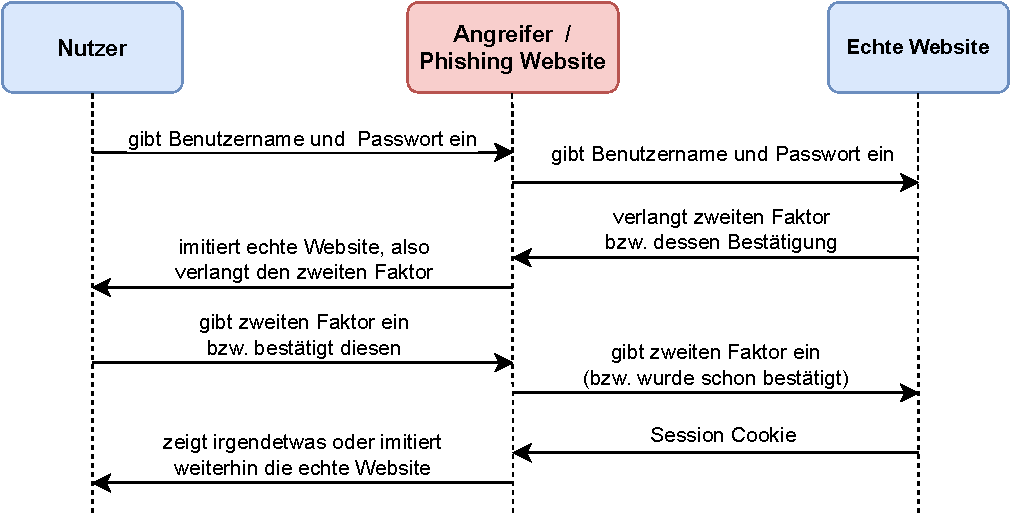
\includegraphics[width=.9\linewidth]{figures/mitmPhishing.pdf}
    \caption[Ablauf einer Phishing-Attacke gegen 2FA]{Ablauf einer Phishing-Attacke gegen 2FA, angelehnt an \autocite[Abb. 1]{Srinivasan}}
    \label{fig: mitm phishing}
\end{figure}
\\\\
Zunächst erstellt der Angreifer eine Website, die die Darstellung und Funktionsweise 
der echten Website imitiert. Dafür gibt es Tools wie Evilginx \autocite{evilginx}. Nun lockt 
der Angreifer das Opfer auf seine Website. Dies geschieht meist durch eine 
Textnachricht, z.B. in Form einer E-Mail. Der Inhalt der Nachricht benötigt einen 
glaubhaften Vorwand, wieso das Opfer sich nun bei der vermeintlich echten Website 
anmelden soll. Zum einen muss die Darstellung eines Links in der E-Mail nicht der 
tatsächlichen Zieladresse entsprechen. Zum anderen kann der Angreifer für seine 
Phishing-Website eine Domain wählen, die der echten Website stark ähnelt, z.B. indem 
man einzelne Buchstaben wie ein kleines \glqq L\grqq{} mit einem großen \glqq I\grqq{} ersetzt. Je nach 
Schriftart im Browser erkennt man keinen Unterschied (siehe Abb. \ref{fig: gitlab}). Dies nennt man auch Typosquatting, wobei es die ursprüngliche Intention von Typosquatting ist, dass der Nutzer eine URL falsch eintippt und auf der Phishing-Website landet. 

\begin{figure}
    \centering
    
\includegraphics[width=.5\linewidth]{figures/gitlab.png}
    \caption[Darstellung zwei ähnlicher Domains]{Darstellung zwei ähnlicher Domains einem unterschiedlichen Zeichen. Abgebildet ist eine Adresszeile des Chrome Browsers mit dem Inhalt \glqq gitlab.com\grqq{} und \glqq gitIab.com\grqq. Ein Unterschied zwischen dem kleinen \glqq l\grqq{} (L) und dem großen \glqq I\grqq{} (i) ist nahezu nicht erkennbar.}
    \label{fig: gitlab}
\end{figure}

Des Weiteren kann die Domain auch einfach eine für den Laien plausible Domain sein, 
wie bspw. \glqq gitlab.login.com\grqq{} anstatt \glqq gitlab.com\grqq{}. Nun denkt das Opfer 
fälschlicherweise, es sei auf der echten Website, und gibt Benutzername und Passwort 
ein. Diese Informationen erhält der Angreifer und übergibt sie an die echte Website. 
Die echte Website zeigt nun an, dass sie den zweiten Faktor verlangt. Diese 
Darstellung wird in Echtzeit auf der Phishing-Website präsentiert. Das Opfer 
bestätigt den zweiten Faktor auf der Phishing-Website z.B. durch die Eingabe eines 
Einmalpassworts oder die Bestätigung einer Push-Nachricht auf dem Smartphone. Der 
Angreifer erhält also auch diese Information und authentisiert sich damit 
vollständig bei der echten Website. Danach kann dem Opfer irgendetwas angezeigt 
werden, z.B. dass der Anmeldungsvorgang fehlgeschlagen sei. Stattdessen kann der Angreifer die echte Website weiterhin imitieren lassen, sodass das Opfer den Angriff in keiner Form bemerkt. 
Der Angreifer speichert im Idealfall die Session-Cookies, um sich später 
ohne Anmeldedaten Zugang zum Account des Opfers zu verschaffen. Durch Tools wie 
Evilginx, sind solche Angriffe einfach zu implementieren und vollständig 
automatisiert. \autocite{Srinivasan}
\\\\
Bis auf das U2F-Verfahren bieten alle üblichen 2FA-Verfahren keinen ausreichenden 
Schutz gegen das Man-In-The-Middle-Phishing. In dieser Arbeit wird ein Konzept für 
Phishing-resistene TOTPs vorgestellt. Dabei wird die Domain der aktuell besuchten 
Website einbezogen.

    \subsection{Passkeys}
        \label{sec: passkeys}
        Passkeys bauen auf den FIDO-Standards auf. Genau genommen basiert es 
auf dem FIDO2-Projekt \autocite{PkFIDO}. Das Ziel ist es, nicht mehr 
auf Passwörter und Benutzernamen sowie 2FA zu setzen, sondern auf eine 
passwortlose Authentisierungsmethode, die angenehmer, schneller und 
sicherer als Passwörter (und 2FA) sind. Passkeys sind 
Phishing-resistent.
\\\\
Das FIDO2-Projekt ähnelt in seinen Grundzügen dem beschriebenen 
U2F-Standard. Es hat allerdings das Ziel, die Identität eines Nutzers 
nicht anhand seines Benutzernamen und Passworts sowie ggf. einem 
zweiten Faktor zu bestimmen, sondern anhand von asymmetrischer 
Kryptographie. D.h. der Nutzer benötigt dann bei der Anmeldung nur noch 
einen privaten kryptographischen Schlüssel und der Dienst kann dessen 
Anmeldung mit dem zugehörigen öffentlichen Schlüssel verifizieren. 
Dabei kommen die zwei Protokolle WebAuthn \autocite{WebAuthnSpec} und 
CTAP2 \autocite{CTAPSpec} zum Einsatz. WebAuthn legt die Kommunikation 
zwischen Dienst (Website) und Client (Browser, Betriebsystem) fest. Der 
Dienst sendet eine Challenge an den Client, dieser identifiziert die 
Domain des Dienstes. Das CTAP2-Protkoll regelt, wie der Client die 
Challenge und Domain an den Authenticator sendet, also das Gerät, auf 
dem der private Schlüssel gespeichert ist. Der Authenticator kann dabei 
ein Smartphone, ein Security Key (z.B. YubiKey) oder selbst das Gerät 
des Clients sein (bspw. mit Windows Hello). Der private Schlüssel 
sollte immer in einem Secure Element \autocite{BSISecEl} gespeichert 
werden, einer eigenständigen physischen Komponente innerhalb des Geräts 
(Authenticators) zur sicheren Verwahrung sensibler Daten. Nun 
verifiziert der Authenticator die Domain und signiert die Challenge mit 
seinem privaten Schlüssel. Anschließend sendet er die signierte 
Challenge zurück an die Client-Instanz und diese leitet sie weiter an 
den Dienst. Der entschlüsselt die Signatur mit seinem öffentlichen 
Schlüssel und vergleicht sie mit der originalen Challenge. Nun ist der 
Client authentifiziert. \autocite{YubiFIDO2}
\\\\
Passkeys Verfahren genau nach der eben beschriebenen Prozedur. 
Allerdings war ein ursprünglicher Gedanke, dass der private Schlüssel 
nie den Authenticator verlässt. Um die Nutzung von Passkeys so angenehm 
wie möglich zu gestalten, wurde diese Beschränkung aufgehoben. Somit 
können Passkeys auf mehreren Geräten über einen Drittanbieter (z.B. 
Google) synchronisiert werden. D.h. der Nutzer muss nur auf einem Gerät 
den Passkey einrichten und kann ihn auf seine anderen Geräte durch den 
Drittanbieter übertragen lassen. So muss der Nutzer nicht für jedes 
Gerät einen Passkey bei einem Dienst einrichten, sondern nur einen 
Passkey für alle seine Geräte. Die Synchronisierung ist Ende-zu-Ende-verschlüsselt, also hat der Drittanbieter keine Einsicht auf die 
privaten Schlüssel. Es sei angemerkt, dass der Nutzer meist auf dem 
Authenticator eine Autorisierung zur Nutzung des privaten Schlüssels 
durchführen muss, z.B. durch einen Scan des Gesichts oder des 
Fingerabdrucks. D.h. nicht, dass die biometrischen Daten für die 
eigentliche Authentisierung beim Online-Dienst genutzt werden. \autocite
{PkFIDORes}
\\\\
Verwendet man ein Smartphone als Authenticator und möchte sich bei 
einem Passkey-losen Gerät (Client) authentisieren, dann muss das 
Smartphone über Bluetooth oder NFC mit dem Client (Browser, 
Betriebssystem des Computers) kommunizieren. Bei der 
Bluetooth-Verbindung vertraut man nicht auf die Sicherheitsmechanismen 
von Bluetooth Low Energy, sondern sichert die Verbindung auf 
Anwendungsebene \autocite{PkFIDORes}. Fraglich bleibt, wie man sich 
bspw. auf einem fremden Computer (ohne Bluetooth, NFC und Kamera) bei 
einem Dienst authentisiert, der bereits Passkeys voraussetzt, weil man 
es bspw. schon mit seinem Smartphone eingerichtet hat. Da Passkeys 
anscheinend eine gute Lösung des gesamten Passwort- und 
2FA-Dilemmas sind, stellt sich die Frage, wieso wir unsere Passwörter 
noch nicht durch Passkeys ersetzt haben (siehe \textcite{FidoRescue} und 
\textcite{lassakaren}).

    \subsection{Verwandte Arbeiten}
        \label{sec: verwandte arbeiten}
        Die Problemstellung, dass bis auf FIDO-basierte Verfahren die 2FA anfällig für Phishing ist, ist 
nicht neu und dennoch existiert sie. Nicht jeder Nutzer möchte bspw. einen Security Key, da er 
ihn die meiste Zeit bei sich tragen muss. Genauso gibt es immer noch viele Websites, die 
Phishing-anfällige Verfahren wie TOTP oder Push nutzen und teilweise nicht einmal die 
Phishing-resistenten Alternativen anbieten. Man handelt nach der Devise \glqq Ein lückenhafter 
Schutz ist besser als gar kein Schutz\grqq{}, und im ersten Augenblick mag diese Behauptung 
stimmen. Aber in Wahrheit verschiebt sich die Angriffsfläche nur: weg von Brute-Force- und 
Wörterbuch-Angriffen (usw.) hin zum Real-time Phishing.
\\\\
2FA-PP steht für 2FA Phishing Prevention und wird in der Arbeit von \textcite{2FAPP} vorgestellt. Es ist ein 
Phishing-resistentes 2FA-Verfahren, bei dem der Browser als zu vertrauende Partei angesehen wird. 
Es kann unter anderem mit One-time Passwords (OTP) kombiniert werden. Es nutzt die Web Bluetooth 
API, damit die Website über den Browser mit dem Smartphone kommuniziert. Nachdem der Nutzer 
seinen Benutzernamen und sein Passwort eingegeben hat, verifiziert die Website diese und sendet 
einen verschlüsselten Javascript-Code an den Browser. Der Browser verlangt vom Smartphone den 
Schlüssel. Das Smartphone sendet den Schlüssel und beginnt eine Zeitmessung. Der Browser erhält 
den Schlüssel, entschlüsselt den Javascript-Code und führt ihn aus. Er sendet das Ergebnis des 
ausgeführten Codes zurück ans Smartphone, das wiederum die Zeitmessung stoppt. Ist das erhaltene 
Ergebnis gültig und die Zeitmessung kleiner als ein bestimmter Grenzwert, gibt das Smartphone der 
Website direkt die Bestätigung, dass der zweite Faktor verifiziert wurde oder das Smartphone 
zeigt bspw. das OTP an, das der Nutzer dann in die Website eintippt. Die Idee scheint 
vielversprechend, da der Nutzer im Idealfall nur Benutzername und Passwort eingeben muss, alles 
2FA-spezifische geschieht im Hintergrund. Problematisch könnte hier allerdings der Fakt sein, 
dass das Smartphone einen Schlüssel an den Browser sendet. Das Senden von privaten Schlüsseln ist eine 
schlechte Praxis \autocite{DIGI}. Außerdem ist auch das Stoppen der Zeit fragwürdig. Der 
Mechanismus basiert darauf, dass der Javascript-Code von einem Angreifer nicht in der kurzen Zeit 
entschlüsselt werden und ausgeführt werden kann. Sollte der Angreifer den Schlüssel erlangen, ist 
dieser Mechanismus hinfällig. Die Idee von 2FA-PP setzt voraus, dass Websites das Konzept von 
2FA-PP unterstützen.
\\\\
Ein ungewöhnlicher Ansatz 2FA nutzerfreundlicher zu gestalten ist 2D-2FA \autocite{2D2FA}. Dabei 
steht 2D für zweidimensional. Die Website zeigt eine Kennung, genauer ein Muster. Das Muster 
funktioniert genauso wie das Wischmuster von Android zum Entsperren des Smartphones. Der Nutzer 
sieht also dieses Muster auf der Website, gibt es in die Smartphone-App ein und dieses generiert 
dann eine PIN, die über das Internet an den Server der Website gesendet wird. Die Idee ist, dass 
der Nutzer nur noch ein Muster auf dem Smartphone eingeben muss für den zweiten Faktor. 
Sicherheitstechnisch gesehen, bringt dieses Konzept allerdings keinen Mehrwert. Im Vergleich zu 
TOTPs tauscht man aus Nutzersicht nur das Eingabegerät. Beim TOTP-Verfahren gibt der Nutzer das 
TOTP in die Website ein, hier gibt der Nutzer prinzipiell ein zufällig generiertes Muster in sein 
Smartphone ein. Das Verfahren schützt genauso wenig vor Phishing wie TOTP. Letztlich ist auch der 
Unterschied nicht revolutionär, ob man als Nutzer nun eine Zahl oder ein Muster ablesen und 
eingeben muss.
\\\\
Ein ebenfalls ungewöhnlicher Ansatz, um 2FA Phishing-resistent zu gestalten und dies mit dem 
Smartphone des Nutzers zu lösen, ist PhotoAuth \autocite{PhotoAuth}. Die Idee ist, die Domain als 
zweiten Faktor zu nutzen. Dabei meldet sich der Nutzer bei einer Website mit Benutzername und 
Passwort an. Die Website sendet dann bspw. per SMS (oder einen anderen Weg) einen Link an das 
Smartphone des Nutzers. Der Nutzer öffnet den Link in einem Browser seines Smartphones. Dort muss 
er der Website erlauben, ein Foto mit seiner Smartphone-Kamera aufzunehmen. Er fotografiert die 
Adresszeile seines PC-Browsers ab, zumindest so, dass die Domain scharf im Bild ist. Dieses Bild 
wird vom Smartphone-Browser dann hochgeladen zum eigentlichen Server, wo sich der Nutzer 
authentisieren möchte. Mithilfe von Optical Character Recognition wird die Domain erkannt und 
geprüft, ob es sich um die echte Domain und nicht um eine Phishing-Domain handelt. D.h. man 
umgeht das Real-time Phishing. Denn bei einem Phishing-Angriff würde der Nutzer unwissentlich 
Benutzername und Passwort an der Angreifer geben, der es an die echte Website weiterleitet. 
Allerdings ist der Kommunikationsweg für den zweiten Faktor ein ganz anderer als der für 
Benutzername und Passwort. Das Foto wird vom Smartphone des Nutzers direkt zum Server der echten 
Website gesendet und dieser würde auf dem Bild feststellen, dass die Domain nicht seiner Domain 
entspricht. Typosquatting könnte je nach Schriftart des Browsers eine ernsthafte Schwachstelle 
sein (siehe Abb. \ref{fig: gitlab}). Man könnte argumentieren, dass der Angreifer einfach selbst 
ein Bild an den Server der echten Website sendet, auf dem die echte Domain zu sehen ist. 
Allerdings kennt er nicht den Link, den der Nutzer per SMS erhalten hat. Denn dieser Link ist für 
jede Anmeldung individuell. Sicherheitstechnisch scheint es bis auf das Typosquatting oder andere 
Möglichkeiten, die Optical Character Recognition zu täuschen, keine Schwachstellen zu geben. 
Hinsichtlich der Nutzerfreundlichkeit ist das Verfahren offensichtlich untauglich, um 
nennenswerte Fortschritte zu erzielen.
\\\\
Zuletzt sei noch 
1Password\footnote{\href{https://support.1password.com/one-time-passwords/}{https://support.1password.com/one-time-passwords/}} 
erwähnt. Es hat das Ziel TOTPs zu vereinfachen. Die Idee ist es, die Geheimnisse online zu 
speichern (und in der App sowie in der Browser-Extension). Nutzt man für die Anmeldung bei einer 
Website die 1Password Browser-Extension, dann erkennt diese automatisch das TOTP-Eingabeelement, 
generiert das TOTP und trägt es automatisch ein. Aus Sicht des Nutzers ist es  angenehm, 
aber hier speichert man seine Geheimnisse remote bei 1Password. D.h. sollte 1Password Opfer eines 
erfolgreichen Angriffs werden, der die Geheimnisse entwendet, ist der zweite Faktor 
kompromittiert. Es sei noch angemerkt, dass 1Password nur gegen monatliche Zahlungen nutzbar ist.

    \subsection{Zusammenfassung}
        \label{sec: grundlagen zusammenfassung}
        Neben den Grundlagen bekannter 2FA-Verfahren wurden deren Probleme erörtert, wie die Anfälligkeit 
gegen Phishing oder schlechte Gebrauchstauglichkeit. Auch wurden Forschungsarbeiten zum Thema 
vorgestellt, die versuchen, 2FA neu zu denken. Passkeys stellen die gesamte 
Zwei-Faktor-Authentisierung in Frage und scheinen eine gute Idee für zukünftige Systeme zu sein. 
Sie könnten deutlich mehr verbreitet sein. Allerdings sind Benutzernamen und Passwörter tief 
verankert und nicht von heute auf morgen wegzudenken. Genauso wenig kann man jeden Webdienst und 
jeden Nutzer dazu zwingen, sich auf \glqq das eine Verfahren\grqq{} zu beschränken.
\\\\
Die im weiteren Verlauf vorgestellte Verbesserung von TOTPs unterscheidet sich dahingehend von 
den bestehenden Systemen und entwickelten Ansätzen, dass sie nahe am TOTP-Verfahren bleibt. 
Letztlich geht es darum, das TOTP automatisch und möglichst mit wenig Nutzerinteraktionen zur 
Website zu transportieren. Dabei soll ein lokales Bluetooth-Netzwerk verwendet werden, ohne dass 
Geheimnisse bei einem Drittanbieter gespeichert werden. Das TOTP bleibt immer noch Bestandteil, 
doch nur im Hintergrund, und kann für eine Fallback-Option nützlich sein. Außerdem hat das später 
vorgestellte Konzept einen Phishing-Schutz für den zweiten Faktor.


\newpage
\section{Verbesserung von Time-based One-time Passwords}
    \label{sec: verbesserung von totps}
    Zunächst werden einige Grundlagen bzgl. der Zwei-Faktor-Authentisierung  geklärt. 
Dabei werden gängige Verfahren sowie deren Stärken und Schwächen bzgl. der Sicherheit 
und Nutzerfreundlichkeit betrachtet. Es wird die Problematik des Phishings vorgestellt 
und anschließend Passkeys sowie verwandte Arbeiten besprochen. 

    \subsection{Herleitung des Konzepts}
        \label{sec: herleitung konzept}
        Im folgenden Abschnitt werden Probleme des TOTP-Verfahrens und Ideen zu deren 
Lösung vorgestellt. Diese Lösungen vereinen sich in einem Konzept zur 
Verbesserung von TOTPs.

\paragraph*{TOTP-App als Grundlage}
\mbox{} \vspace{0.1cm} \\
Zunächst stellt sich die Frage, wieso das TOTP-Verfahren und insbesondere die 
TOTP-Apps für Erweiterungen geeignet sind. Zuerst sei genannt, dass das 
Smartphone als der zweite Faktor fungiert. D.h. man benötigt keinen neuen 
Gegenstand wie einen Security-Key für die 2FA. Diese TOTP-Apps sind unabhängig 
von den Diensten, bei denen sich ein Nutzer authentisieren möchte. Ein Dienst muss nur das TOTP-Verfahren unterstützen, ansonsten hat er 
keinen Einfluss auf die App. Somit kann der Nutzer seine 2FA-Vorgänge mithilfe 
einer App erledigen, anstatt für jeden Dienst eine eigene App zu nutzen. Das ist 
nämlich der Fall beim Push-Verfahren. Wobei es auch Push-Verfahren wie Authy One 
Touch gibt, bei denen eine App für mehrere Dienste genutzt werden kann. 
Andererseits benötigt man mit den TOTP-Apps keinen Mobilfunkempfang oder 
Internetzugang, da das Einmalpasswort von der App selbst berechnet wird.  
Betrachtet man nun die Probleme des 
TOTP-Verfahrens, lassen sich diese mit einigen Erweiterungen lösen.

\paragraph*{Ablesen und Eintippen des TOTPs}
\mbox{} \vspace{0.1cm} \\
Ein wesentliches Problem ist das Ablesen und Eintippen des 
Einmalpassworts. Die App generiert das TOTP und der Nutzer muss es bei jedem 
Authentisierungsvorgang in die Website eingeben. Zum einen ist das 
zeitintensiv und unbequem \autocite{Reese}, zum anderen lenkt es auch von der Aufgabe ab, die der 
Nutzer eigentlich erledigen möchte. Dazu kommt, dass potentiell die Ziffern des 
Einmalpasswort falsch abgelesen bzw. falsche Ziffern eingegeben werden.

\paragraph*{Automatische Übertragung des TOTPs}
\mbox{} \vspace{0.1cm} \\
Es ist fraglich, wieso der Nutzer überhaupt das TOTP übertragen soll. 
Stattdessen kann die App das TOTP an den Browser senden und dieser schreibt es 
automatisch in das Eingabefeld. Also benötigt man eine geeignete Technologie zur 
Datenübertragung, die von den meisten Smartphones und Computern unterstützt wird 
oder leicht nachzurüsten ist. Infrage kommen dabei NFC, Bluetooth und prinzipiell 
auch der Weg über einen Server im Internet. QR-Codes sind unpassend, da sie nur 
unidirektional kommunizieren und der Nutzer aktiv werden muss. NFC ist zwar in 
den meisten modernen Smartphones integriert, aber wird nicht von jedem Laptop und 
noch seltener von Desktop-PCs unterstützt. Man kann NFC-Chips in 
Form von USB-Geräten an den PC anschließen. Allerdings sind sie für den mobilen 
Gebrauch eher unhandlich. Der Weg, das TOTP über einen Server zu übertragen, 
würde wieder einen Internetzugang erfordern und, wie später noch ausgeführt wird, 
die Angriffsfläche für MFA-Fatigue öffnen. Bluetooth dagegen wird von den meisten 
modernen Smartphones und Laptops unterstützt. Gegebenenfalls kann es auch mit kleinen 
erschwinglichen USB-Geräten nachgerüstet werden. Zudem sendet Bluetooth je nach 
Konfiguration und Bedingungen über Reichweiten von wenigen Metern bis hin zu 
mehreren Hundert Metern \autocite{btEstimator}, während NFC nur mit Reichweiten von bis zu $2~cm$ \autocite{nfcForum} 
agiert. Bluetooth ist auch bereits in den Browsern Chrome, Edge und Opera 
integriert und nennt sich Web Bluetooth \autocite{webBt}. Daher fällt die 
Entscheidung auf Bluetooth als Funktechnologie.

\paragraph*{Nutzer als letzte Sicherheitsinstanz}
\mbox{} \vspace{0.1cm} \\
Einerseits sollte das Einmalpasswort nicht ohne eine Interaktion des Nutzers an 
den Browser gesendet werden. Denn auch wenn die Verbindung zwischen der App und 
dem Browser sicher ist, könnte jemand mit Zugang zum Computer des Nutzers 
versuchen, sich bei einem Dienst anzumelden, während der Nutzer dies nicht 
bemerkt. Andererseits ist es sogar die Überlegung wert, doch ohne jegliche 
Nutzerinteraktion das TOTP an Browser zu senden. Voraussetzung wäre natürlich, 
dass die Verbindung zwischen App und Browser Ende-zu-Ende verschlüsselt, 
authentisiert und resistent gegen jegliche kompromittierende Angriffe ist, wie 
bspw. Replay-Attacken oder Man-In-The-Middle-Attacken beim Schlüsselaustausch. 
Ist das gegeben, könnte theoretisch nur der Computer bzw. Browser das TOTP vom 
Smartphone verlangen. Andererseits könnte es ein Risiko sein, wenn der Computer 
bzw. der Browser mit Malware infiziert ist. D.h. es bedarf einer Abwägung aus Sicherheit und Komfort: soll die App einfach TOTPs an einen vertrauten Browser senden dürfen oder soll der Nutzer jedes TOTP freigeben, bevor die App es an den Browser sendet.

\paragraph*{Transformation zum Push-Verfahren}
\mbox{} \vspace{0.1cm} \\
Ein weiteres Problem bei den gewöhnlichen TOTP-Apps ist, dass der Nutzer die App 
erst suchen, öffnen und den entsprechenden Account aus einer Liste wählen muss, 
um an das Einmalpasswort zu gelangen. Das kann behoben werden, indem man die 
TOTP-App mithilfe der Bluetooth-Funktionalität in eine App verwandelt, die aus 
Sicht des Nutzers einer App mit Push-Verfahren gleicht. Sobald der Browser 
erkennt, dass der Nutzer das TOTP eingeben muss, sendet er der App einen Befehl, 
damit diese eine Benachrichtigung anzeigen kann. So kann der Nutzer auf die 
Benachrichtigung tippen und muss nur noch zustimmen, dass das TOTP an den Browser 
übertragen werden soll. Dadurch könnte das neue Konzept zusätzlich Zeit bei der 
Authentisierung einsparen  (vergl. Abb. \ref{fig: reese zeiten} Push vs. 
TOTP) und weniger Interaktionen vom Nutzer verlangen. Das Problem, das Push-Apps der MFA-Fatigue ausgesetzt sind, gilt hier nur noch für den lokalen Bereich, wenn der Angreifer in der Lage ist, das Smartphone des Nutzers per Bluetooth zu erreichen.

\paragraph*{Schutz gegen Phishing}
\mbox{} \vspace{0.1cm} \\
Nachdem nun einige Ansätze zu einer verbesserten Nutzerfreundlichkeit und einem 
geringeren Zeitaufwand vorgestellt wurden, muss auch das Problem des fehlenden 
Schutzes vor Phishing (siehe Kap. \ref{sec: phishing}) gelöst werden. Prinzipiell 
muss der Browser (nicht die Website) als vertrauenswürdige Partei angesehen 
werden. Richtet der Nutzer dieses neue Verfahren bei einem Webdienst ein, dann 
soll der Browser den Benutzernamen und die Domain der Website an die 
Smartphone-App senden. Den Benutzernamen ermittelt der Browser, wenn sich der 
Nutzer beim Webdienst anmeldet. Die App erhält bei der Einrichtung das Geheimnis, 
indem sie den QR-Code auf der Website scannt. Die App speichert den Benutzernamen 
und die Domain zusammen mit dem Geheimnis. Meldet sich der Nutzer nach der 
Einrichtung an, empfängt die App vom Browser die Domain der Website und den 
Benutzernamen. Die App prüft, ob sie diese Domain bereits kennt. Ist dies der 
Fall, zeigt die App dem Nutzer die Benachrichtigung an und sendet bei dessen 
Zustimmung das entsprechende TOTP an den Browser. Kennt die App die Domain nicht, 
dann sollte sie den Nutzer warnen, dass er sich auf einer Phishing-Website 
befindet.

\paragraph*{Kein Zeitdruck und unnötiges Warten}
\mbox{} \vspace{0.1cm} \\
Zuletzt seien noch zwei zeitkritische Probleme von Interesse. Generell entfernt 
das neue Konzept den wahrnehmbaren Zeitdruck. Der Nutzer muss das TOTP nicht mehr 
abtippen und sieht auch keinen Countdown mehr, der eventuell Stress auslösen 
kann. Außerdem entfällt das Problem, dass der Nutzer warten muss, wenn das TOTP 
nur noch wenige Sekunden gültig ist (z.B. 5s). In diesem Fall wartet der Nutzer oft 
auf das nächste Einmalpasswort, weil er es in der verbleibenden Zeit nicht in den 
Browser übertragen könnte. Man könnte vermuten, dass dieses Problem in anderer 
Weise auch für das neue Konzept gilt. Zum Beispiel könnte die App das 
Einmalpasswort genau dann senden, wenn es nur noch 1s gültig ist. Dann wird es 
zwar automatisch in die Website eingegeben, aber falls die Übertragung und die 
Bestätigung der Eingabe mehr als $1~s$ dauern, wäre das Einmalpasswort nicht mehr 
gültig. Aber der RFC 6238 empfiehlt, dass der Webdienst das TOTP des aktuellen 
30s-Zeitfensters sowie das TOTP im Zeitfenster davor und danach akzeptiert. Also 
ist das Einmalpasswort aus dem eben genannten Beispiel noch ca. $30~s$ gültig.

    \subsection{Konzept zur Verbesserung von Time-based One-time Passwords}
        \label{sec: funktionsweise konzept}
        Das Konzept zur Verbesserung adressiert die Probleme des TOTP-Verfahrens und 
beabsichtigt, die vorangegangenen Ideen zu vereinen, so dass es als neuer Standard für 
TOTPs verwendet werden kann.
Damit wird die Vision geschaffen, dass aktuelle Browser und 
TOTP-Apps dieses Konzept in Zukunft unterstützen. Vor allem ist der Browser  essentiell, da er die kontrollierende Partei verkörpert. Das Konzept soll folgende Ziele verwirklichen:
\begin{itemize}
    \item Sicherheit gegen Phishing
    \item Bessere Nutzererfahrung und mehr Nutzerfreundlichkeit durch reduzierte Arbeitslast und weniger Interaktionen
    \item schnellere Authentisierung durch die automatische Übertragung des TOTPs
\end{itemize}
Das Konzept unterteilt sich wie auch das übliche TOTP-Verfahren in Einrichtung und Authentisierungsvorgang.


        \subsubsection{Einrichtung}
            \label{sec: konzept einrichtung}
            In Abb. \ref{fig: konzept setup} ist ein Sequenzdiagramm dargestellt, das den Ablauf des Konzepts für 
die Einrichtung des erweiterten TOTP-Verfahrens beschreibt. An dem Prozess der Einrichtung nehmen vier Parteien teil. Die App auf dem Smartphone des Nutzers und der Nutzer selbst sowie der Browser als eigene Partei und die Website.

\begin{figure}
    \centering
    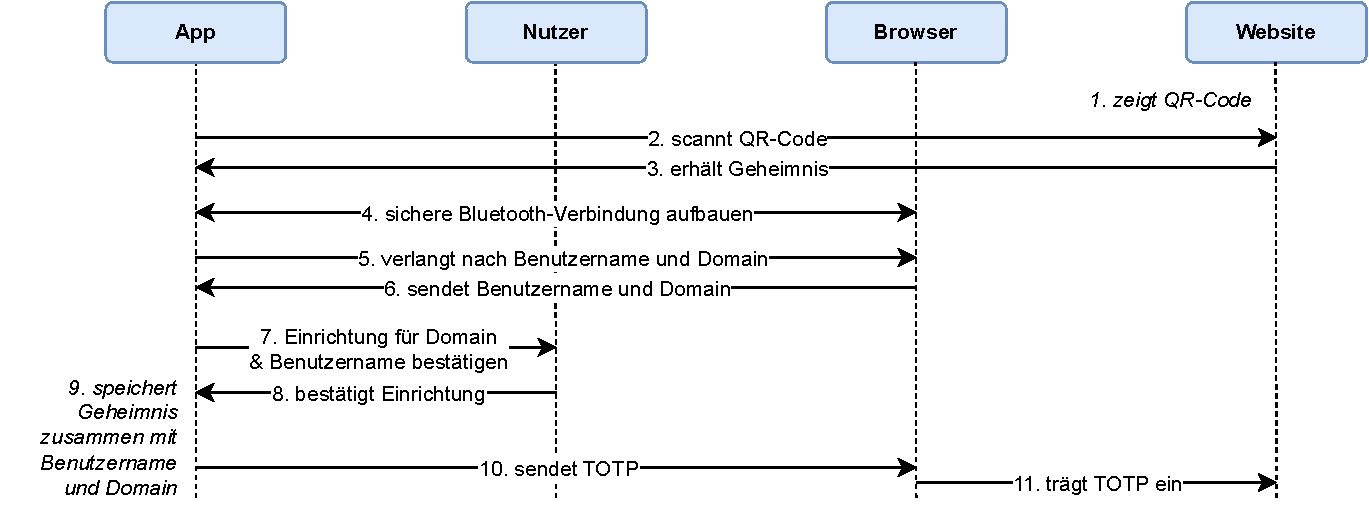
\includegraphics[width=1\linewidth]{figures/konzept_setup.pdf}
    \caption[Einrichtungsprozess des Konzepts zu einem neuen TOTP-Verfahren]{Einrichtungsprozess des Konzepts zu einem neuen TOTP-Verfahren}
    \label{fig: konzept setup}
\end{figure}

\paragraph*{Übertragung des Geheimnisses (1. - 3.)}
\mbox{} \vspace{0.1cm} \\
Üblicherweise wird beim TOTP-Verfahren der QR-Code gescannt, um das Geheimnis von 
der Website in die App zu übertragen. Wenn man das TOTP-Verfahren gänzlich neu 
standardisieren möchte, dann könnte man auch überlegen, ob der Browser den 
QR-Code ausliest bzw. das Geheimnis direkt von der Website erhält, ohne dass der 
Nutzer es sieht. Das Geheimnis könnte dann zusammen mit der Domain des 
Webdienstes und dem Benutzernamen an die App gesendet werden. Möchte man eine 
Lösung implementieren, die den aktuellen Standard nur erweitert, dann bleibt man 
bei der QR-Scan-Methode.

\paragraph*{Aufbau einer sicheren Bluetooth-Verbindung (4.)}
\mbox{} \vspace{0.1cm} \\
Zunächst stellt sich die Frage, welche Art von Bluetooth verwendet werden soll. 
Neben dem Bluetooth Classic bietet sich auch Bluetooth Low Energy (BLE) an, das 
sogar mit dem Web Bluetooth Standard kompatibel ist. Bluetooth bietet 
Sicherheitsfunktionen für eine möglichst sichere Kommunikation an und die 
Bluetooth Special Interest Group (SIG) ist bemüht, die Sicherheit von Bluetooth 
stetig zu verbessern. Allerdings ist eine Ende-zu-Ende-Verschlüsselung auf 
Anwendungsebene empfehlenswert \autocite[9]{siliconLabs} \autocite{androidBt}, da Hardware mit älteren 
Bluetooth-Versionen (bspw. 4.0)  immer noch im Umlauf ist und diese viele 
Schwachstellen aufweisen \autocite{Lonzetta}. Dazu könnte man den Transport Layer Security (TLS) 
Standard nutzen, der jedoch eine Zertifikatskette voraussetzt. Eine andere Lösung 
wäre eine Public-Key-Verschlüsselung, die ggf. beim initialen Schlüsselaustausch 
einige Schwachstellen aufweist, dafür aber unabhängig von Zertifikaten 
funktioniert. Letztendlich sollten die Schutzziele der Informationssicherheit, 
also Vertraulichkeit, Integrität und Verfügbarkeit \autocite[98]{VonSolms}, erfüllt werden. 
Die Bluetooth-Verbindung kann auch schon eher als Schritt 4 
(siehe Abb. \ref{fig: konzept setup}) etabliert werden.
Die Verbindung soll sich 
automatisch wiederherstellen, sobald zwei bekannte Parteien wieder in 
Reichweite sind. Natürlich muss dafür Bluetooth bei beiden Geräte aktiviert sein.

\paragraph*{Benutzername und Domain (5. \& 6.)}
\mbox{} \vspace{0.1cm} \\
Der Browser prüft pro besuchter Domain stetig, ob im HTML-Quellcode ein 
Eingabefeld für den Benutzernamen erscheint. Durch die Popularität von 
Passwort-Managern haben Webdienste auf ihrer Login-Seite meist eine einheitliche 
Markierung gesetzt, damit ein Passwort-Manager programmatisch das Eingabefeld für 
den Benutzername identifizieren kann. Dies funktioniert mit dem HTML-Attribut 
\lstinline{autocomplete}. Es kann verschiedene einheitliche Werte wie \lstinline
{username} für den Benutzernamen annehmen \autocite{htmlAutocomplete}. So kann im 
Konzept der Browser den Benutzernamen feststellen. Sollte es einmal nicht 
funktionieren, dann muss der Browser (oder die App) den Nutzer nach dem 
Benutzernamen fragen.
Die Domain dagegen kann der Browser einfach mit folgendem Javascript-Code 
ermitteln.
\begin{lstlisting}[numbers=none]
let url = document.location.href;
let domain = new URL(url).hostname.replace("www.", "");
\end{lstlisting}

\paragraph*{Bestätigung der Einrichtung (7. \& 8.)}
\mbox{} \vspace{0.1cm} \\
Diese Schritte sind eher optional. So kann der Nutzer noch sichergehen, ob der 
Benutzername korrekt ist und ob er wirklich den Zwei-Faktor-Schutz aktivieren 
möchte. Man könnte dem Nutzer auch erklären, was er bei Verlust des Smartphones 
tun kann.

\paragraph*{Speichern des Geheimnisses (9.)}
\mbox{} \vspace{0.1cm} \\
Die App speichert nun das Geheimnis zusammen mit der Domain und dem Benutzernamen ab. So kann später beim Authentisierungsvorgang mithilfe von Domain und 
Benutzername das notwendige Geheimnis identifiziert werden. Das Geheimnis kann 
verschlüsselt gespeichert werden.

\paragraph*{Übertragung des ersten TOTPs (10. \& 11.)}
\mbox{} \vspace{0.1cm} \\
Traditionell verlangen Dienste nach einem initialen TOTP, um sicherzugehen, dass 
der Nutzer das Geheimnis in seiner App gespeichert hat und der 2FA-Schutz nun 
aktiviert werden kann. Würde man einen neuen Standard entwerfen, könnte man diese 
Schritte auch im Hintergrund erledigen, ohne dass der Nutzer ein Eingabefeld für 
das initiale TOTP sieht. Die App könnte über Bluetooth eine Bestätigung an den 
Browser senden und dieser an die Website.

        \subsubsection{Authentisierungsvorgang}
            \label{sec: konzept authentisierungsvorgang}
            Nach einer erfolgreichen Einrichtung kann der Nutzer sich in Zukunft mithilfe des neuen Konzepts einfacher authentisieren bei Eingabe des zweiten Faktors (dem TOTP). Das Konzept sieht dabei den in Abb. \ref{fig: konzept login} dargestellten Ablauf vor.

\begin{figure}
    \centering
    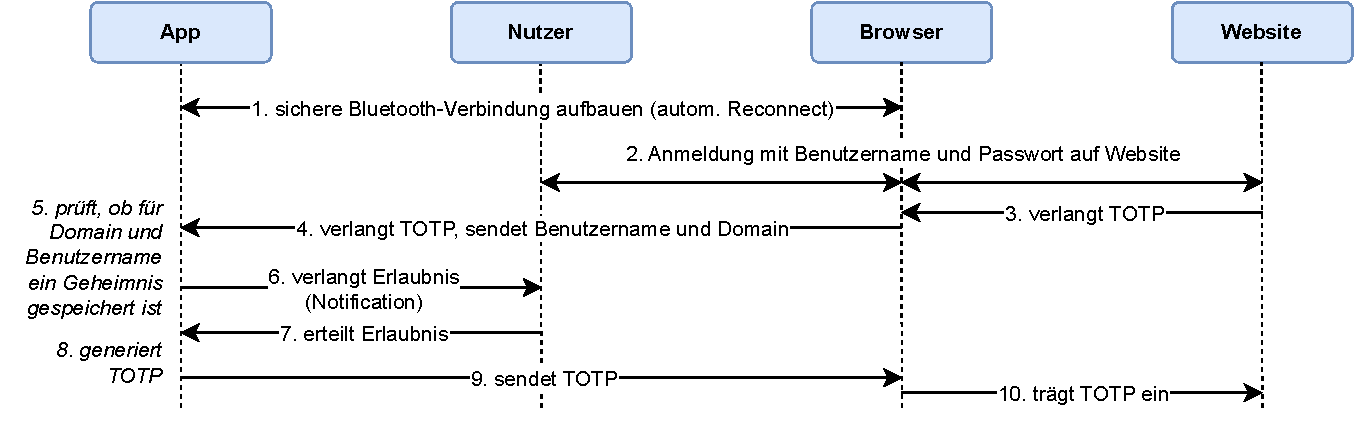
\includegraphics[width=1\linewidth]{figures/konzept_login.pdf}
    \caption[Authentisierungsvorgang des Konzepts zu einem neuen TOTP-Verfahren]{Authentisierungsvorgang des Konzepts zu einem neuen TOTP-Verfahren}
    \label{fig: konzept login}
\end{figure}

\paragraph*{Aufbau einer sicheren Bluetooth-Verbindung (1.)}
\mbox{} \vspace{0.1cm} \\
Wie bereits bei der Einrichtung beschrieben, bauen App und Browser eine sichere 
Bluetooth-Verbindung auf. Es ist von Vorteil, wenn Bluetooth sowohl auf dem 
Smartphone als auch auf dem Computer aktiviert ist, damit App und Browser sich 
ohne eine weitere Nutzerinteraktion automatisch neu verbinden. Des Weiteren senkt 
es die Nutzerinterkationen, wenn die App immer im Hintergrund läuft, damit der 
Nutzer die App nicht öffnen muss, nur um sie mit dem Browser zu verbinden.

\paragraph*{Anmeldung mit Benutzername und Passwort (2.)}
\mbox{} \vspace{0.1cm} \\
Wie gewohnt meldet sich der Nutzer mit Benutzername und Passwort bei der Website 
an und erfüllt somit den ersten Faktor der 2FA.

\paragraph*{Verlangen des TOTPs (3. - 5.)}
\mbox{} \vspace{0.1cm} \\
Wie bereits bei der Einrichtung beschrieben, kann der Browser das Eingabeelement 
des Benutzernamens durch den HTML-Quellcode erkennen. Mit dem HTML-Attribut  
\lstinline{autocomplete="one-time-code"} kann der Browser auch das Eingabeelement des 
Einmalpassworts erkennen. Allerdings ist bei Webdiensten der Gebrauch des 
Attributwertes \lstinline{one-time-code} nicht so sehr vertreten wie \lstinline{username}. D.h. Webdienste müssen konsequent das Eingabeelement des TOTPs 
markieren, damit das Konzept funktioniert.
Hat der Browser das TOTP-Eingabeelement erkannt, verlangt der das TOTP von der 
App. Zusätzlich übergibt er Benutzername und Domain, damit die App das zugehörige 
Geheimnis in ihrem Speicher identifizieren kann. Im Fall, dass der Nutzer sich auf einer Phishing-Website befindet, würde die App kein Geheimnis in ihrem Speicher finden, da sie nur die Domain der echten Website kennt und nicht die Domain der Phishing-Website. Demnach kann die App auch kein TOTP generieren und warnt den Nutzer.

\paragraph*{Freigabe des TOTPs durch den Nutzer (6. \& 7.)}
\mbox{} \vspace{0.1cm} \\
Besitzt die App ein Geheimnis für die empfangene Domain und den zugehörigen Benutzernamen, dann fragt sie den Nutzer um Erlaubnis für die Übertragung des 
TOTPs an den Browser. Über eine Notification kann die Anfrage an den Nutzer 
gestellt werden. Je nach Betriebssystem kann der Nutzer direkt mit der 
Notification interagieren und so die Anfrage bestätigen und ablehnen, ohne die 
App öffnen zu müssen \autocite{appleNotify,androidNotify}. 
Diese Schritte zur Freigabe des TOTPs sind nur für den Fall notwendig, dass der 
Browser durch Malware kompromittiert wurde oder dass es einem Angreifer in der 
Nähe durch eine Sicherheitslücke gelingt, sich als vertrauter Browser auszugeben. 
In einem solchen Fall ist die Bedrohung für den Nutzer nicht zwingend 
offensichtlich, aber anhand des Zeitpunktes des Empfangens der Notification, weiß 
der Nutzer, ob diese Anfrage von ihm stammt oder nicht. Ausnahme ist hier der 
Fall, dass der Angreifer gezielt zur selben Zeit wie der Browser des Nutzers das 
TOTP von der App verlangt.

\paragraph*{Übertragung des TOTPs an die Website (8. - 10.)}
\mbox{} \vspace{0.1cm} \\
Die App generiert nun das TOTP und sendet es an den Browser. Dieser trägt es dann 
automatisch in das TOTP-Eingabeelement ein. Theoretisch könnte Schritt 10 auch 
gänzlich im Hintergrund geschehen, so dass der Nutzer das Eingabefeld nie 
wahrnehmen muss.

\paragraph*{Anmerkung: Smartwatch als 5. Partei}
\mbox{} \vspace{0.1cm} \\
Verknüpft man sein Smartphone mit einer Smartwatch, kann man für gewisse Situationen annehmen, noch mehr Zeit zu sparen. Ist das Smartphone bspw. in der Tasche oder der Hostentasche, bestätigt man die Notification aus Schritt 6 mit Hilfe der Smartwatch.
        \subsubsection{Alternativer Authentisierungsvorgang (Fallback)}
            \label{sec: konzept fallback}
            Für den Fall, dass beim Authentisierungsvorgang keine Bluetooth-Verbindung 
zwischen App und Browser hergestellt werden kann, gibt es eine alternative 
Lösung. In Abb. \ref{fig: konzept fallback} ist der Ablauf des alternativen 
Authentisierungsvorgangs dargestellt.
\\\\
\begin{figure}
    \centering
    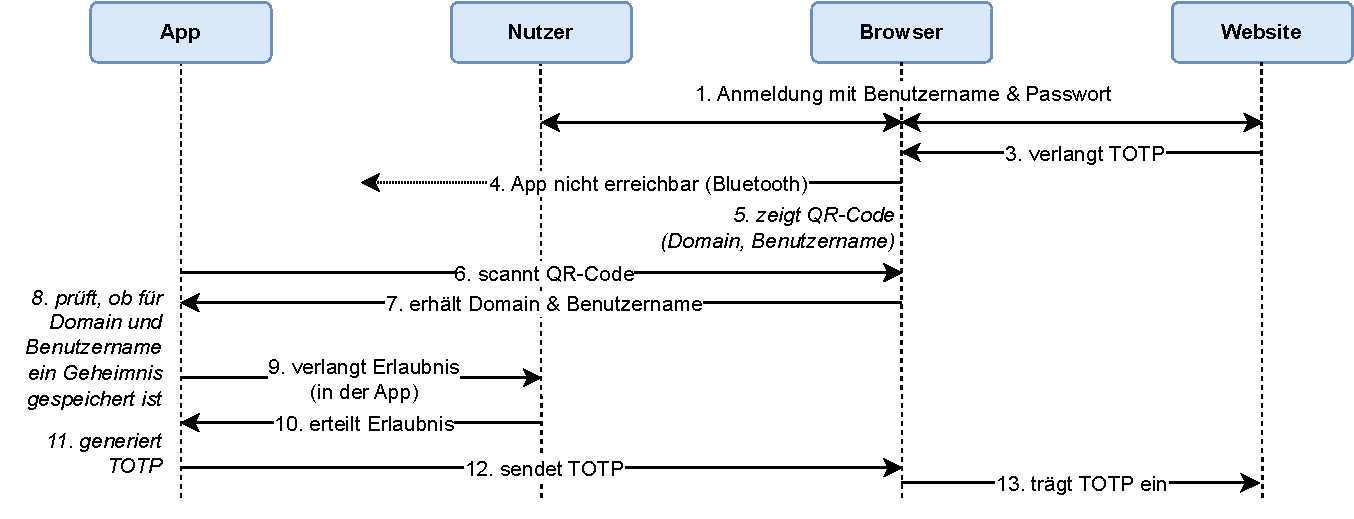
\includegraphics[width=1\linewidth]{figures/konzept_login_fallback.pdf}
    \caption[Fallback des Konzepts zu einem neuen TOTP-Verfahren]{Alternativer Authentisierungsvorgang (Fallback) des Konzepts zu einem neuen TOTP-Verfahren}
    \label{fig: konzept fallback}
\end{figure}
Bis auf die Schritte 4, 5, 6 und 9 sind alle Schritte identisch mit den 
entsprechenden Schritten des normalen Authentisierungsvorgangs. In Schritt 3 
erkennt der Browser, dass das TOTP verlangt wird und versucht eine 
Bluetooth-Verbindung zur App herzustellen. In diesem Fall scheitert der 
Verbindungsaufbau und der Browser bietet dem Nutzer den alternativen 
Authentisierungsvorgang an. Dazu zeigt der Browser einen QR-Code an, der 
letztlich nur den Benutzernamen und die Domain enthält (Schritt 5). Wichtig ist 
hier zu erwähnen, dass der Browser den QR-Code anzeigt und nicht die Website. 
Sollte es eine Phishing-Website sein, könnte sie im QR-Code die Domain der echten 
Website angeben, die sie imitiert. Daher vertraut man der Website nicht. Der Nutzer 
scannt den QR-Code (Schritt 6) und es öffnet sich die App. Nun hat die App die 
Domain und den Benutzernamen erhalten und es wird wie beim normalen 
Authentisierungsvorgang fortgefahren. Ausnahme sei Schritt 9. Da die App momentan 
schon geöffnet ist, kann sie direkt den Nutzer um Erlaubnis fragen, um das TOTP 
an den Browser zu senden. Es muss nicht extra eine Notification erstellt werden. 
\\\\
Es existiert noch eine Schwachstelle bei Schritt 3, indem man sich der potentiellen 
Unwissenheit des Nutzers bedient. Eine Phishing-Website könnte anstatt eines 
TOTP-Eingabeelements einen QR-Code anzeigen und den Nutzer auffordern, diesen zu 
scannen. Der QR-Code enthält die Domain der echten Website und den eben eingegebenen 
Benutzernamen. Der Nutzer weiß aber in diesem Szenario nicht, dass er keine QR-Codes 
von der Website scannen darf bei der Authentisierung, also scannt er den QR-Code. Die 
App würde ihm nun das TOTP anzeigen und er würde es unwissentlich in die 
Phishing-Website eingeben. Es ist denkbar, bei einer früheren Verbindung zwischen 
Browser und App asymmetrische Schlüssel auszutauschen und Informationen im QR-Code zu 
signieren, die dann von der App beim Scan entschlüsselt und verifiziert werden. So 
weiß die App, dass der QR-Code vom Browser stammt. Denn die Phishing-Website kennt 
nicht den Schlüssel des Browsers und kann demnach keinen gültigen QR-Code erstellen. 
Allerdings bleibt die Frage offen, wie man gegen dieses Szenario vorgeht, wenn der 
Nutzer den vorliegenden Browser in Kombination mit seiner App das erste Mal nutzt. 

    \subsection{Forschungsfragen \& Forschungsansatz}
        \label{sec: forschungsansatz}
        Das vorgestellte Konzept zur Verbesserung von zeitbasierten Einmalpasswörtern 
soll als aktuelle Implementierung umgesetzt werden. Während es wünschesnwert ist, dass Browser-Anbieter das Konzept als neuen Standard unterstützen, erfolgt die Überprüfung der Machbarkeit in Form eines Prototypen. 
D.h. es soll eine Lösung geschaffen werden, die nicht erst in entfernter Zukunft 
nutzbar ist, sondern jetzt.
Anhand dieser Implementierung wird untersucht, ob die beschriebenen Änderungen am 
gewöhnlichen \mbox{TOTP-Verfahren} einen Mehrwert für den Nutzer generieren. Es stellen sich somit die folgenden Forschungsfragen:
\begin{itemize}
    \item Wie kann eine eine solche gegenwärtige Implementierung mit einem Schutz gegen \\MITM-Phishing realisiert werden?
    \item Welche Auswirkungen hat die Implementierung auf die Nutzererfahrung und die Nutzerfreundlichkeit?
    \item Welche Auswirkungen hat die Implementierung auf die Task Completion Time?
\end{itemize}
Das Konzept und die zugehörige Implementierung zielen darauf ab, Schutz vor Phishing zu bieten. Allerdings wird dieser Aspekt weder technisch noch bzgl. der Nutzererfahrung weiter untersucht.
\\\\
Daraus werden folgende Hypothesen abgeleitet:
\begin{itemize}
    \item[(a)] Der Prototyp des neuen Verfahrens für zeitbasierte Einmalpasswörter ist nutzerfreundlicher als das gewöhnliche TOTP-Verfahren.
    \item[(b)]  Der Prototyp des neuen Verfahrens für zeitbasierte Einmalpasswörter benötigt bzgl. der Authentisierungsvorgänge weniger Zeit als das gewöhnliche TOTP-Verfahren.
\end{itemize}
Um den Forschungsfragen nachzukommen, wurde eine Studie mit Probanden geplant. 
Dazu muss das neue TOTP-Verfahren unterschieden werden in seine Einrichtung und 
seine eigentliche Nutzung beim Login. Das heißt, es ist sinnvoll die Studie wie \textcite{Reese} in einen Termin zur Einrichtung, einer mehrtägigen Nutzungsphase und einen Abschlusstermin aufzuteilen. Voraussetzung zur Durchführung der Studie ist die funktionierende Implementierung 
des neuen TOTP-Verfahrens, die gegenwärtig funktioniert und nicht voraussetzt, dass Browser das neue Konzept als Standard unterstützen.
Die Auswahl der Probanden soll sich auf Nutzer beschränken, die bereits Erfahrung 
mit zeitbasierten Einmalpasswörter haben, speziell mit den TOTP-Apps (nicht SMS 
oder Email). Durch Interviews und Fragebögen kann so ermittelt werden, inwiefern 
die Implementierung des neuen TOTP-Verfahrens eine Verbesserung zu dem 
gewöhnlichen TOTP-Verfahren darstellt.

\paragraph*{Erwartungen an die Studie}
\mbox{} \vspace{0.1cm} \\
Da nun der Forschungsansatz vorgestellt wurde, stellt sich die Frage, welche 
Erwartungen an die Studie gestellt werden. Was soll die Studie bewirken
\\\\
Zum einen gibt es die Zeitmessung der Einrichtungs- und 
Authentisierungsvorgänge. Allerdings wird sie ohne eine zweite Probandengruppe, 
die das gewöhnliche TOTP-Verfahren testet, keinen echten Vergleichswert haben. 
Dennoch kann ihre Dimension als Vergleich für ähnliche Studien genutzt werden. 
Die Zeitmessung basiert auf einem Logging: also was tut der Nutzer beim 
Webdienst. So können auch fehlgeschlagene Anmeldungen beziffert werden. D.h. man 
kann keine Aussage darüber treffen, ob das neue TOTP-Verfahren nun tatsächlich 
schneller als das gewöhnliche ist. Mit einer zweiten Probandengruppe für das 
gewöhnliche Verfahren könnte man eine Aussage treffen. Mit den 
Fragen im Interview kann zumindest festgestellt werden, ob die Teilnehmer das 
neue TOTP-Verfahren schneller oder langsamer empfinden und aus welchen Gründen.
\\\\
Bezüglich der Nutzerfreundlichkeit / Gebrauchstauglichkeit und der 
Nutzererfahrung geben die SUS und der UEQ eine gute Vorstellung davon, wie die 
beiden Verfahren sich hinsichtlich des Authentisierungsvorgangs unterscheiden. 
Auch gibt das Interview in der Abschlussveranstaltung Aufschluss darüber, aus 
welchen Gründen die Teilnehmer eines der Systeme bevorzugen. Die Fragebögen (SUS 
und UEQ) zur Einrichtung sind eher informativ, da bereits vermutet wird, dass das 
Einrichtungsverfahren mit der bereitgestellten Implementierung etwas aufwendiger 
ist als die Einrichtung des gewöhnlichen Verfahrens. Die Fragen 
und Beobachtungen bezüglich der Einrichtung dienen dazu, die Probleme der zu 
identifizieren und neue Ideen zu sammeln, um den Vorgang zukünftig leichter 
zu gestalten.

\newpage
\section{Implementierung}
    \label{sec: implementierung}
    Zunächst werden einige Grundlagen bzgl. der Zwei-Faktor-Authentisierung  geklärt. 
Dabei werden gängige Verfahren sowie deren Stärken und Schwächen bzgl. der Sicherheit 
und Nutzerfreundlichkeit betrachtet. Es wird die Problematik des Phishings vorgestellt 
und anschließend Passkeys sowie verwandte Arbeiten besprochen. 

    \subsection{Kommunikationsarchitektur}
        \label{sec: implementierung architektur}
        Im Gegensatz zum Konzept umfasst der Prototyp mehr Nutzerinteraktionen. Der 
Nutzer muss vor allem bei der Einrichtung mehr mit der Extension 
interagieren, als der Nutzer im Konzept mit dem Browser interagieren muss. 
Bei der Authentisierung sind die Nutzerinteraktionen des Prototyps identisch 
mit dem Konzept. Bis auf die Tatsache, das Blue TOTP die Bluetooth-Verbindung 
zwischen App und Extension noch nicht eigenständig aufbaut, wenn die Geräte 
früher schon einmal verbunden waren. Dafür muss der Nutzer noch händisch 
Sorge tragen. Prinzipiell sei noch erwähnt, dass Bluetooth Low Energy 
verwendet wird. Die App agiert als Peripheral Device (in Bluetooth Low Energy die 
Server-Rolle) und die Extension als Central Device (Client-Rolle). Diese 
Entscheidung wird in den folgenden Kapiteln begründet.

\paragraph*{Einrichtung}
\mbox{} \vspace{0.1cm} \\
In Abb. \ref{fig: prototyp kommunikation ablauf einrichtung} ist die 
Kommunikationsarchitektur sowie Nutzerinteraktionen bei der Einrichtung 
dargestellt.
\begin{figure}[h]
    \centering
    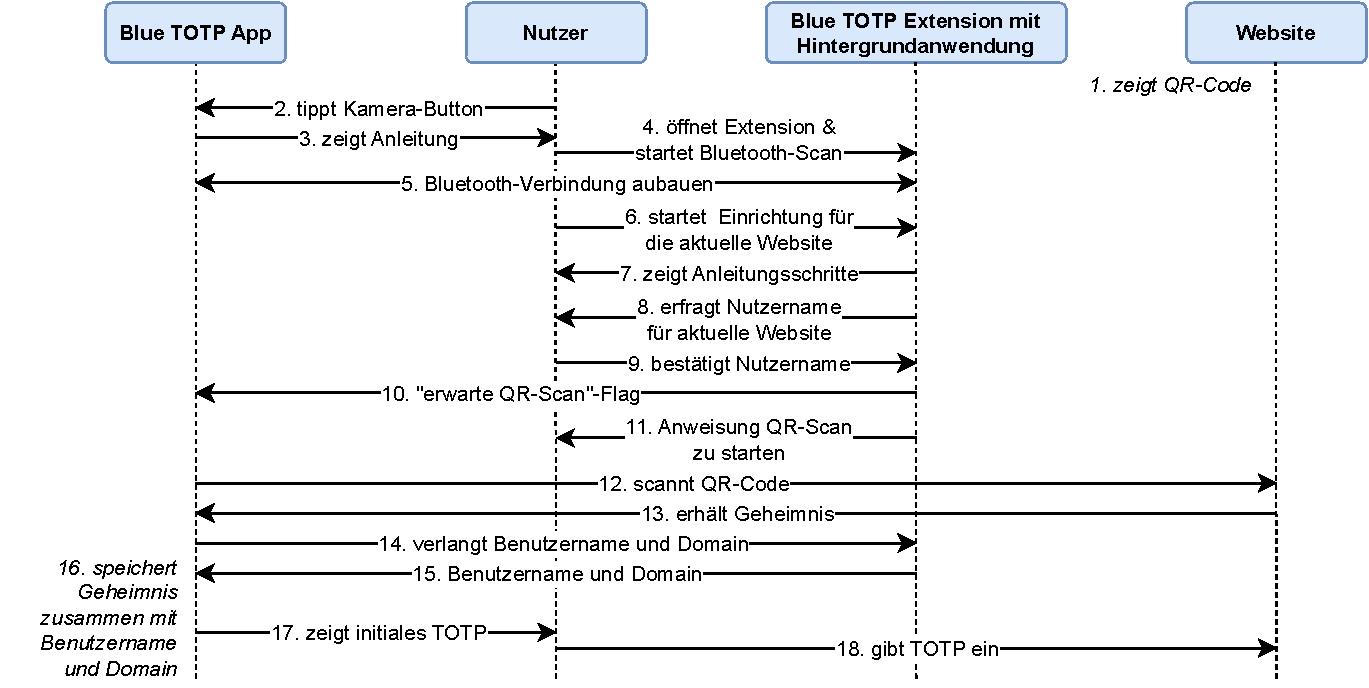
\includegraphics[width=1\linewidth]{figures/impl/blue_totp_setup.pdf}
    \caption[Einrichtungsprozess des Prototyps Blue TOTP]{Einrichtungsprozess des Prototyps Blue TOTP}
    \label{fig: prototyp kommunikation ablauf einrichtung}
\end{figure}
Die Schritte müssen nicht zwingend in dieser Reihenfolge ablaufen, allerdings 
haben alle Probanden der später vorgestellten Studie diesen Ablauf gewählt. 
Die Ausgangssituation sei, dass der Nutzer bereits die 2FA-Einrichtung auf 
der Website begonnen hat und die Website ihm nun einen QR-Code anzeigt und 
das initiale TOTP verlangt.
\\\\
Der Nutzer sieht den QR-Code und öffnet seine Authenticator-App, also Blue 
TOTP. Diese zeigt rechts unten, wie in Abb. \ref{fig: blue totp app 
screenshot nicht verbunden} zu sehen, einen Button mit einer Kamera als 
Symbol. Nach Antippen des Buttons erscheint eine Anleitung (vergl. 
Abb. \ref{fig: blue totp app screenshot anleitung}. Diese besagt, dass der 
Nutzer Bluetooth aktivieren und die Blue TOTP Chrome Extension öffnen soll. 
Dort folgt er der Benutzeroberfläche, um mit der Extension den Bluetooth-Scan 
zu starten, und stellt die Verbindung zum Smartphone (genauer zur App) her. 
Diese Verbindung ist unsicher, da dies für die Studie nicht von Bedeutung 
ist. In einer realen Anwendung sollte diese Verbindung sicher sein, wie es 
das Konzept vorsieht. Erst, wenn Smartphone und App verbunden sind, kann die 
Einrichtung mittels Blue TOTP in der Extension gestartet werden (vergl. 
Abb. \ref{fig: blue totp ext screenshot verbunden}). Die einzelnen Schritte 
der Anleitungen sind in Anhang \ref{anh: blue totp ext screens} zu sehen. Ziel 
der Anleitung ist es, dem Nutzer allgemeingültig zu erklären, wie er bei 
einer Website zur 2FA-Einrichtung gelangt. Danach erfragt die Extension noch 
den Benutzernamen für die Website. Dieser wird automatisch bei der Anmeldung 
auf der Website erkannt und in diesem Schritt der Anleitung dem Nutzer 
gezeigt. Man kann den Namen ggf. ändern. Dies sollte man aber nur tun, wenn 
nicht der korrekte Nutzername  für die Website vorgeschlagen wird. 
Andernfalls funktioniert der Authentisierungsvorgang später nicht. Nun 
fordert die Extension den Nutzer auf, erneut den Kamera-Button der App 
anzutippen, damit die App den QR-Code scannen kann. Damit die App jetzt nicht 
wieder ihre initiale Anleitung anzeigt, erhält sie von der Extension eine 
Nachricht per Bluetooth, dass der QR-Scan freigegeben ist (Schritt 10). Der 
restliche Verlauf (12. bis 16.) ist identisch mit dem Konzept. Ausnahmen sind 
Schritt 17 und 18. Hier zeigt die App das aktuelle TOTP an, das der Nutzer 
nun ablesen und in die Website eingeben muss. Die Einrichtung ist somit 
abgeschlossen.

\paragraph*{Authentisierung}
\mbox{} \vspace{0.1cm} \\
Der Authentisierungsvorgang unterscheidet sich kaum von der Vorgabe des 
Konzepts. Der Ablauf der Authentisierung ist in Abb. \ref{fig: prototyp 
kommunikation ablauf auth} dargestellt.
\begin{figure}[h]
    \centering
    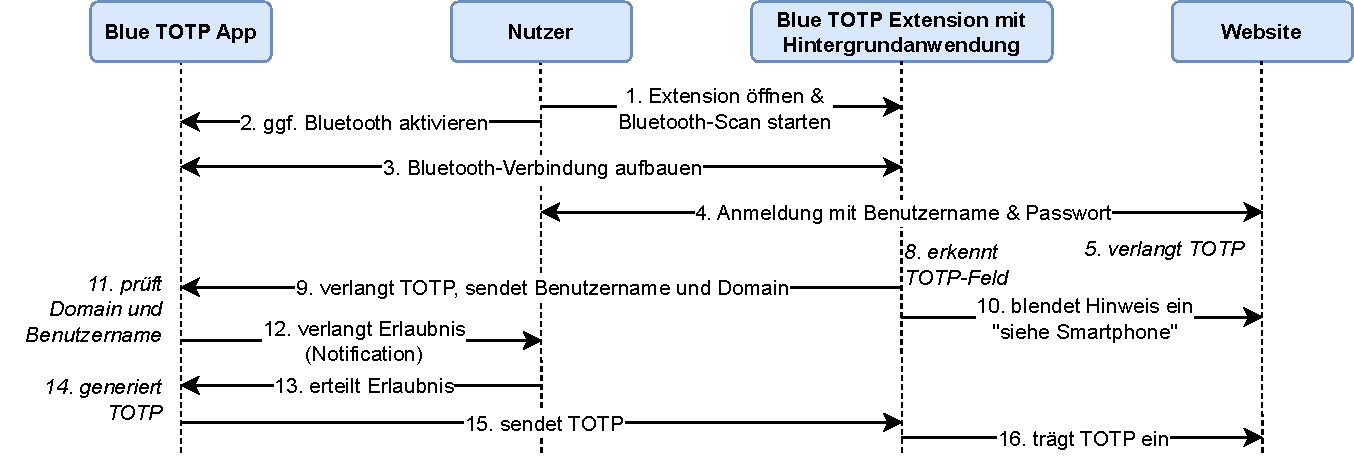
\includegraphics[width=1\linewidth]{figures/impl/blue_totp_login.pdf}
    \caption[Authentisierungsprozess des Prototyps Blue TOTP]{Authentisierungsprozess des Prototyps Blue TOTP}
    \label{fig: prototyp kommunikation ablauf auth}
\end{figure}
Der wesentliche Unterschied zum Konzept ist nur, dass der Nutzer die 
Bluetooth-Verbindung initialisieren muss, indem er die Extension öffnet und 
mit ihr nach seinem Smartphone scannt (Schritt 1). Gegebenenfalls muss er, 
wie in Schritt 2 beschrieben, Bluetooth auf dem Smartphone aktivieren. Die 
App läuft theoretisch immer im Hintergrund. Allerdings kann es je nach 
Android-Version und Konfigurationen vorkommen, dass Android diesen 
Hintergrundprozess beendet, um Energie zu sparen. Dann muss der Nutzer die 
App zusätzlich öffnen. Alle restlichen Schritte sind identisch mit dem 
Konzept bis auf Schritt 10. Hier wird dem Nutzer durch die Extension ein 
Hinweis innerhalb der Website angezeigt, dass er die Notification (aus 
Schritt 12) in seinem Smartphone bestätigen soll. Des Weiteren sei angemerkt, 
dass auch hier die Bluetooth-Verbindung nicht sicher ist, da es für die 
Studie unbedeutend bleibt.
\\\\
Im Fall, dass dem Nutzer kein Bluetooth zur Verfügung steht, gibt es einen 
Fallback in der Blue TOTP App. Jedoch ist er nur experimentell umgesetzt und 
verfügt daher über keinen Phishing-Schutz. Wie beim traditionellen 
TOTP-Verfahren muss der Nutzer das TOTP ablesen und selbst in den Browser 
eintragen.

    \subsection{Smartphone Application}
        \label{sec: implementierung app}
        Die grundlegenden Aufgaben der Blue TOTP App sind die gleichen Aufgaben, wie die 
einer gewöhnlichen TOTP-App: QR-Codes scannen, deren Geheimnis speichern und dann 
TOTPs generieren. Allerdings muss die Blue TOTP App noch weiterer Fähigkeiten 
bemächtigt werden. Zum einen muss sie per Bluetooth kommunizieren können sowie 
bestenfalls immer im Hintergrund laufen und das Bluetooth-Advertising betreiben 
(als Bluetooth-\glqq Server\grqq{} erreichbar sein). Zumindest muss sie das 
Advertising solange ausführen, bis sie sich mit einer Blue TOTP Extension 
verbindet. Zum anderen muss sie bei der Einrichtung den Benutzernamen und die 
Domain der Website von der Extension empfangen und diese zusammen mit dem Geheimnis 
speichern. Denn nur so kann sie später bei der Authentisierung immer für genau ein 
Paar aus Benutzername und Domain genau ein gespeichertes Geheimnis identifizieren 
und das TOTP generieren.
\\\\
Dazu wurden verschiedene One-time Password (OTP) Apps untersucht wie 
Aegis\footnote{\href{https://github.com/beemdevelopment/Aegis}{https://github.com/beemdevelopment/Aegis}}, FreeOTP\footnote{\href{https://github.com/freeotp/freeotp-android}{https://github.com/freeotp/freeotp-android}}, und FreeOTP+\footnote{\href{https://github.com/helloworld1/FreeOTPPlus}{https://github.com/helloworld1/FreeOTPPlus}}. 
Letztlich fiel die Entscheidung auf FreeOTP+, da es kein Onboarding hat und sehr 
minimalistisch gestaltet ist und trotzdem einen großen Funktionsumfang bietet. Das 
direkte Anzeigen des TOTPs wurde entfernt. Stattdessen muss man nun über das 
Overflow Menu (Menü mit drei übereinander liegenden Punkten) beim gewünschten 
Token-Eintrag auf \glqq Token anzeigen\grqq{} tippen. Dann erscheint der Screen in 
Abb. \ref{fig: blue totp app screenshot token}. Dessen Design mit dem abnehmenden 
Kreisbogen um die ablaufende Zeit, die das TOTP noch gültig ist, wurde Apps wie 
Authy nachempfunden. Auch Funktionen wie der Export oder Import von TOTP 
Geheimnissen wurden entfernt, um die App für die Studie auf das Wesentliche zu 
begrenzen. Es wurde, wie in Abb. \ref{fig: blue totp app screenshot nicht verbunden} 
bzw. Abb. \ref{fig: blue totp app screenshot verbunden} zu sehen, eine Statusbar 
bzgl. der Bluetooth-Verbindung zur Extension eingebaut. Prinzipiell wurde hier und 
auch bei der Extension mit Symbolen und Farben gearbeitet, um Menschen mit 
Sehschwächen nicht zu benachteiligen. Die Idee, ein Symbol für den 
Verbindungsstatus in die App Bar zu setzen (obere Leiste der App, mit Text und 
Buttons), wurde verworfen. Das Symbol wirkte durch die Anwesenheit der anderen 
Buttons in der App Bar auch wie ein Button.
\begin{figure}[h]
    \centering
    \begin{subfigure}{.23\textwidth}
      \centering
      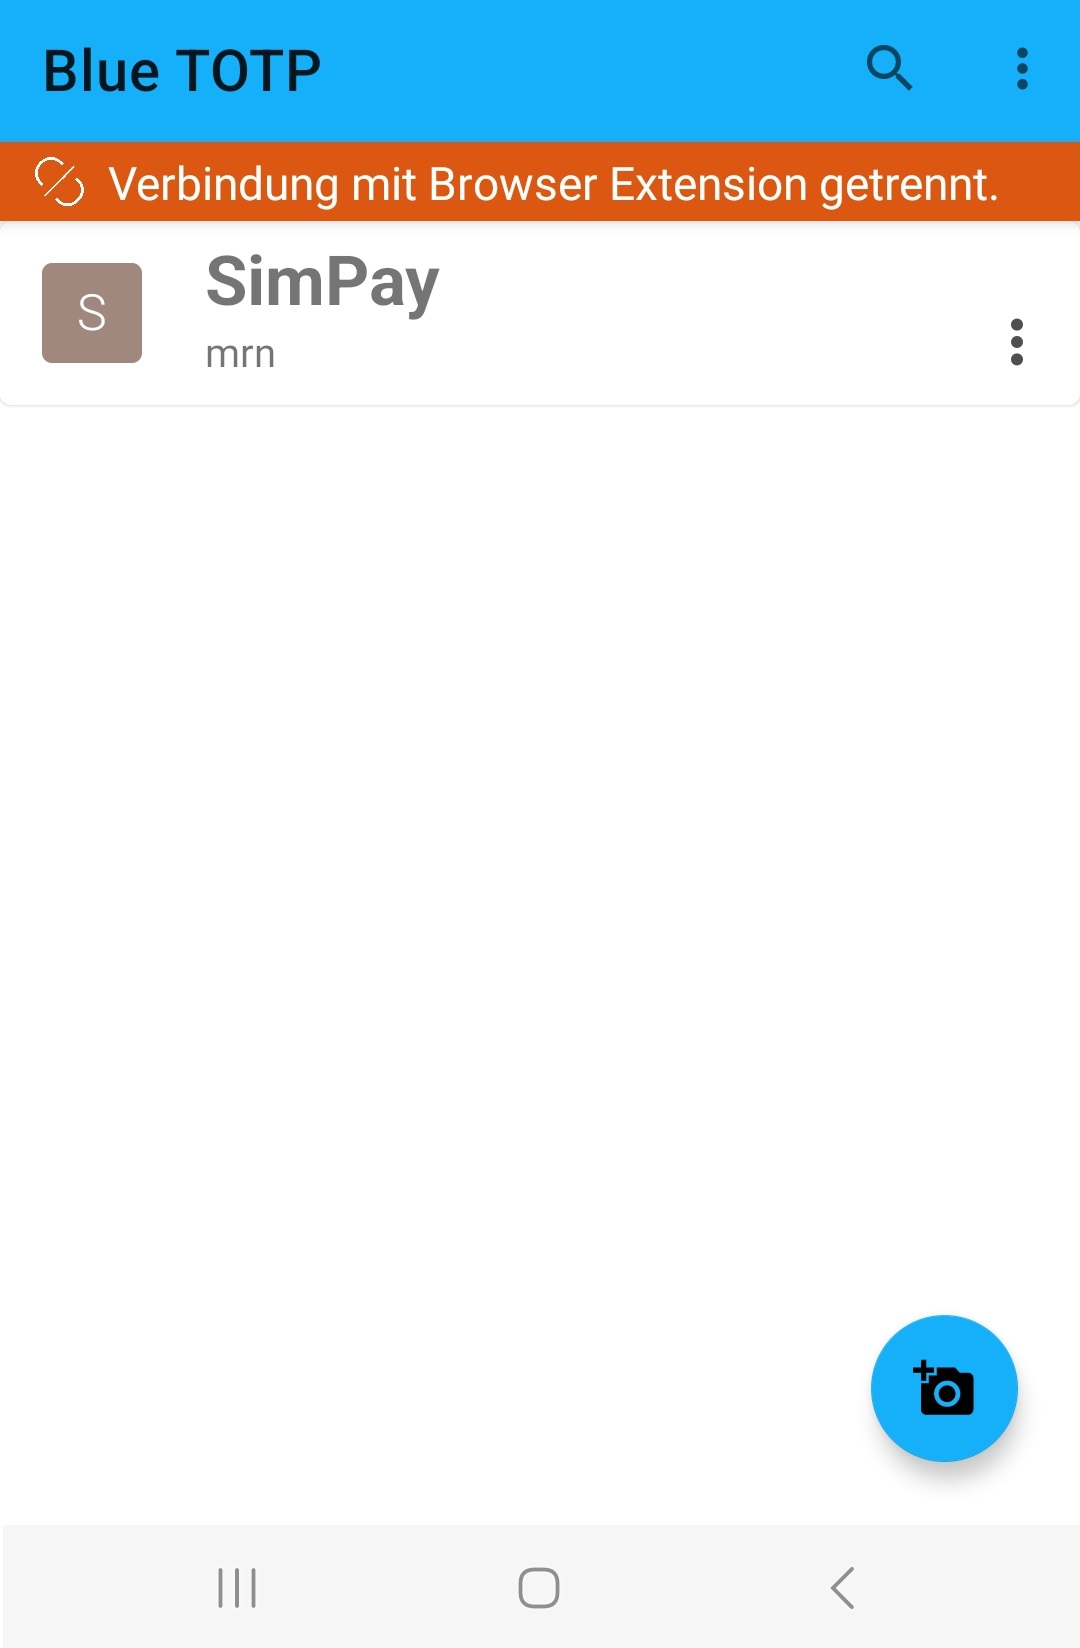
\includegraphics[width=.95\linewidth]{figures/impl/screenshot_app_nicht_verbunden.jpg}
      \caption{Main (nicht verbunden)}
      \label{fig: blue totp app screenshot nicht verbunden}
    \end{subfigure}%
    \begin{subfigure}{.23\textwidth}
      \centering
      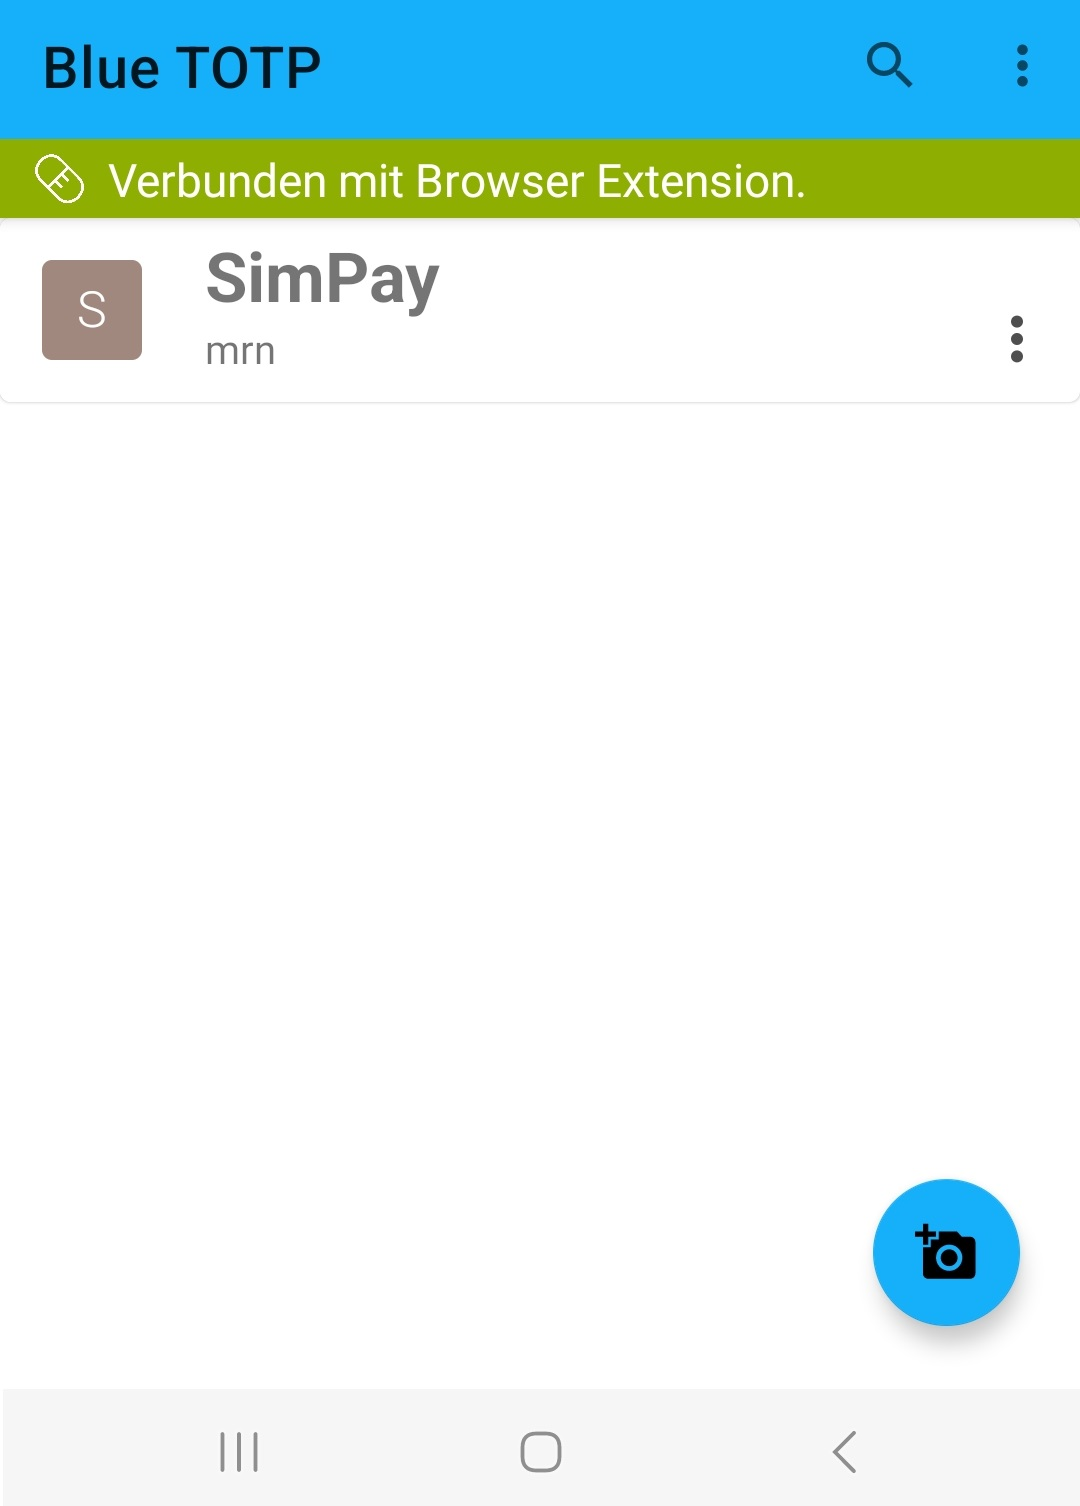
\includegraphics[width=.95\linewidth]{figures/impl/screenshot_app_verbunden.jpg}
      \caption{Main (verbunden)}
      \label{fig: blue totp app screenshot verbunden}
    \end{subfigure}
    \begin{subfigure}{.23\textwidth}
        \centering
        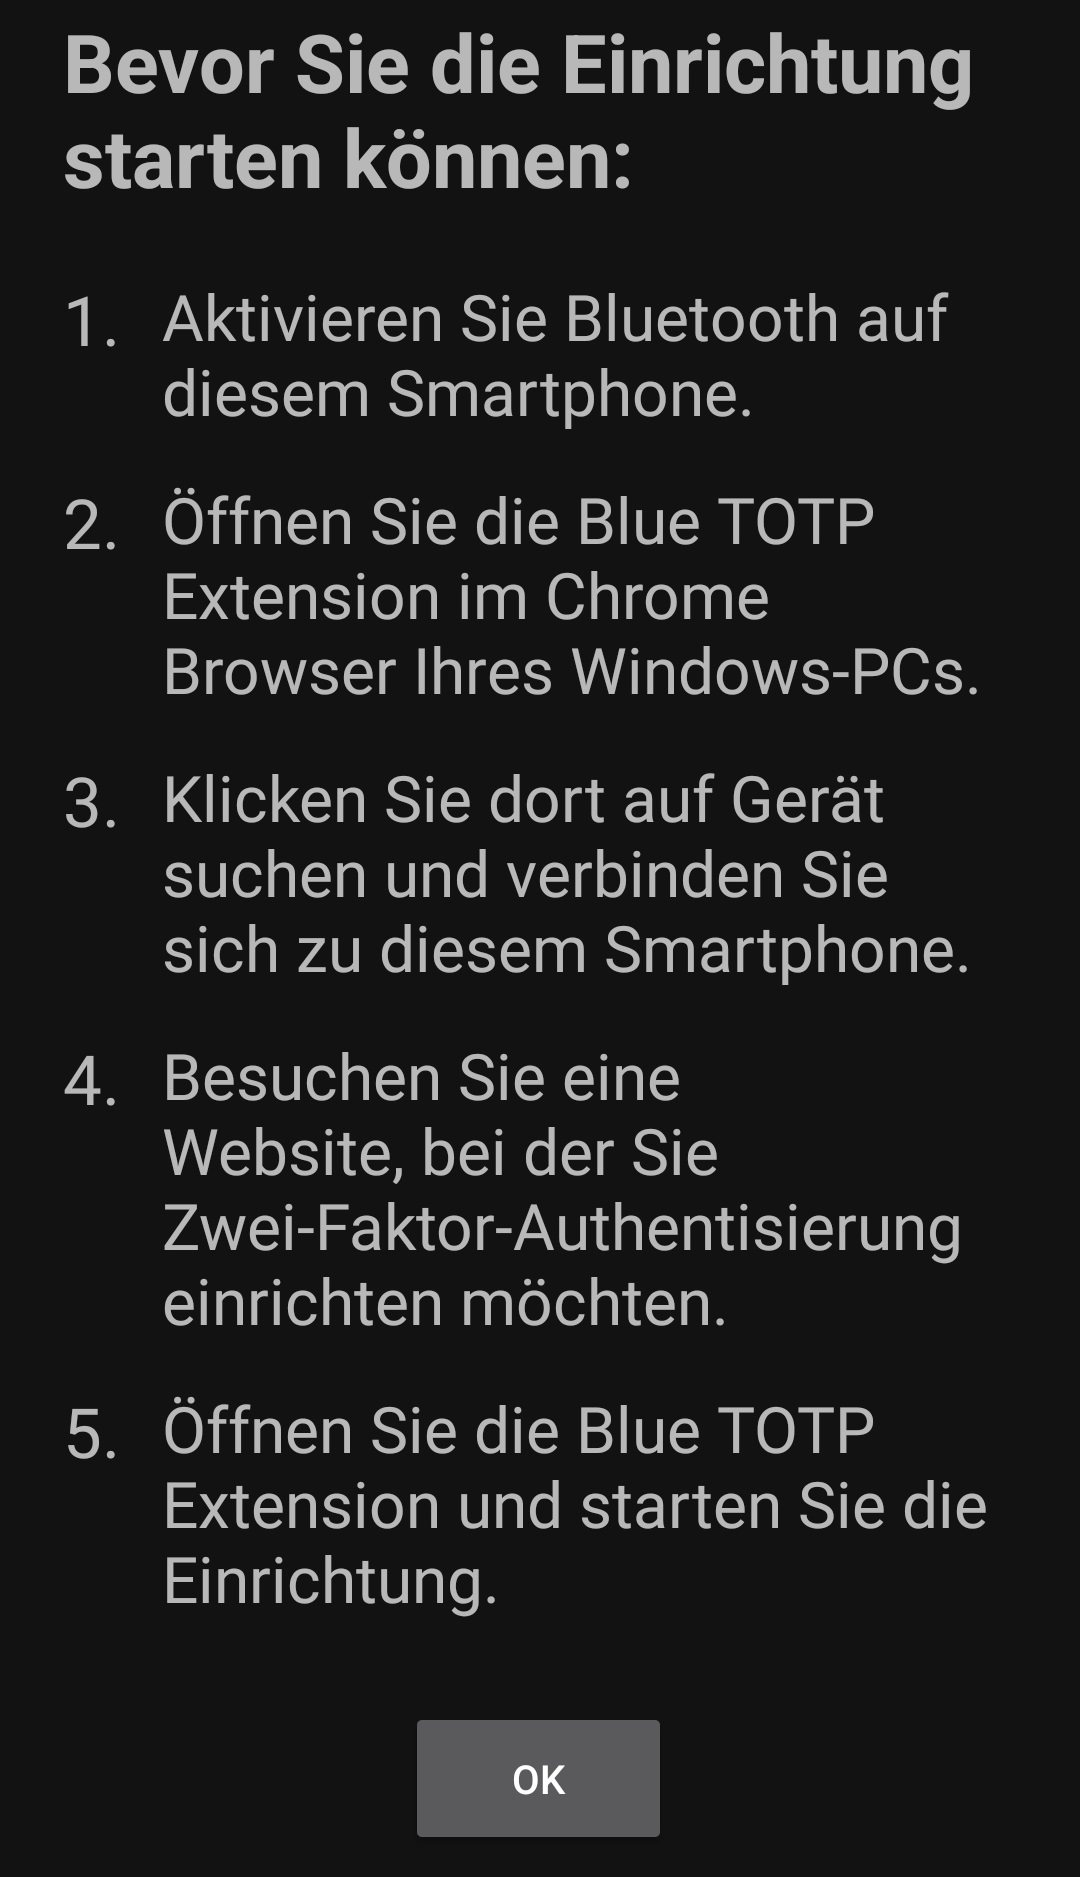
\includegraphics[width=.95\linewidth]{figures/impl/screenshot_app_anleitung.jpg}
        \caption{Anleitung}
        \label{fig: blue totp app screenshot anleitung}
    \end{subfigure}
    \begin{subfigure}{.23\textwidth}
        \centering
        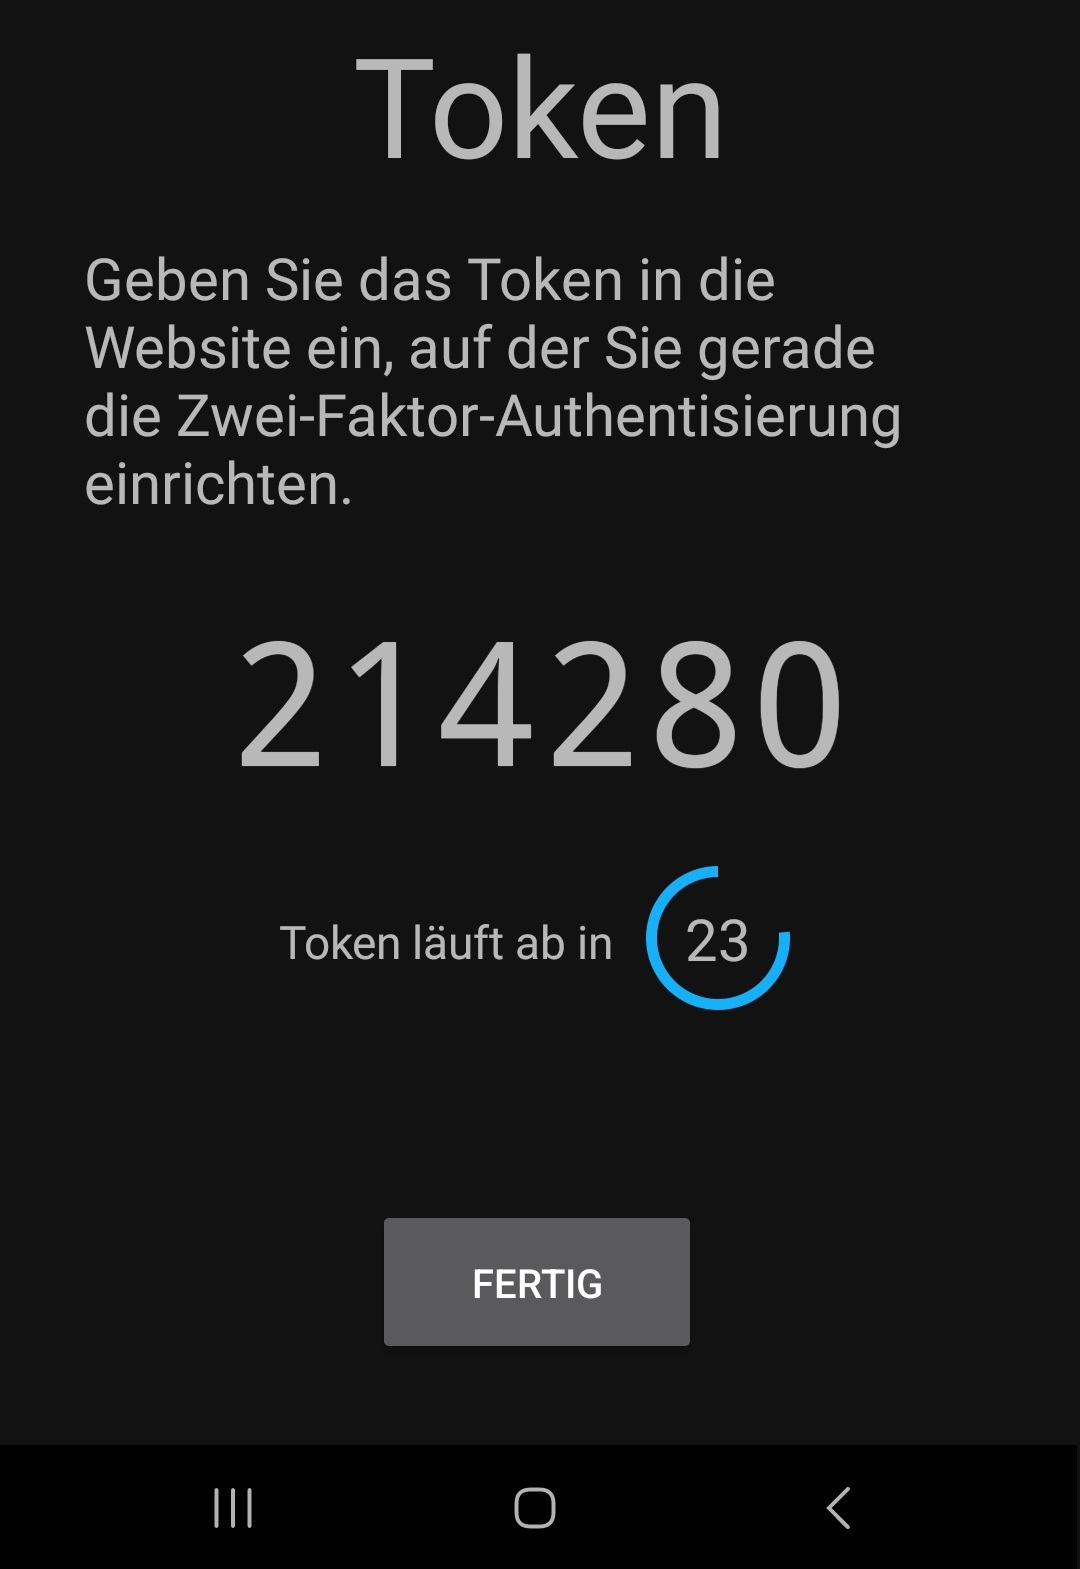
\includegraphics[width=.95\linewidth]{figures/impl/screenshot_app_token.jpg}
        \caption{Token}
        \label{fig: blue totp app screenshot token}
    \end{subfigure}
    \caption[Screens der Blue TOTP App]{Screens/Activities der Blue TOTP App}
    \label{fig: blue totp app screenshots}
\end{figure}

Für den Hintergrundprozess mit der gesamten Bluetooth-Funktionalität wurde ein 
sogenannter Foreground Service gewählt. Auf dem Testgerät konnte dieser tagelang 
laufen und wurde nicht einmal durch Android beendet. Wie bereits erwähnt, variiert 
dieses Verhalten je nach Konfiguration des Android Systems. Leider zeigt diese Art 
von Service permanent eine Notification an, dass die App aktiv ist. Ein passendes 
Beispiel ist ein Music Player. Solange man Musik hört, wird die Notification 
angezeigt und man kann mit dieser sogar interagieren (Musik pausieren, Songs 
überspringen). Für die Blue TOTP App ist der Foreground Service im Nachhinein keine 
gute Wahl. Allerdings ist es nicht leicht (oder nur dem Autor unbekannt), Prozesse 
in Android permanent laufen zu lassen, da es gegen das Prinzip verstößt, 
Arbeitsspeicher, Rechenleistung und Batterie effizient zu verwalten. Der Foreground 
Service schien die einzige plausible Lösung dafür zu sein. Die App wurde 
hauptsächlich mit Android 13 getestet, unterstützt aber auch Android 8.0. 
Allerdings benötigt die Blue TOTP App die Funktion des Bluetooth Low Energy 
Advertisings. Ältere Geräte (auch Geräte mit Android 8.0) verfügen nicht zwingend 
über Bluetooth-Hardware, die diese Funktion unterstützt.

    \subsection{Browser-Extension}
        \label{sec: implementierung ext}
        Bei der Einrichtung und der Authentisierung muss der Browser dem Konzept zufolge 
den Benutzernamen und die Domain an die App senden. Außerdem muss er beim Login das 
HTML-Eingabeelement erkennen und das TOTP von der App verlangen. Also ist der 
Browser die Partei, der man vertrauen muss. Es muss also bei der Umsetzung der 
Browser-Partei bedacht werden, dass sie potentiell nicht von einer anderen Partei 
negativ beeinflusst werden kann.
\\\\
Nun benötigt man zunächst einen Browser, der Bluetooth unterstützt. 
Chromium\footnote{\href{https://www.chromium.org/chromium-projects/}{https://www.chromium.org/chromium-projects/}} 
ist eine Open Source und beinhaltet die sogenannte Web Bluetooth API. Aber wie kann 
man den Browser die nötigen Abläufe durchführen lassen? Man könnte von Chromium 
eine eigene Instanz erstellen (Fork) und die Software für unsere Browser-Rolle 
integrieren. Für das Konzept wäre das die optimale Option, da man den Browser 
vollständig kontrolliert. Für eine Lösung, die im Alltag funktionieren soll, würde 
es bedeuten, dass der Nutzer einen neuen Browser benötigt, nur um unser neues 
TOTP-Verfahren zu nutzen. Also unpassend. Stattdessen entschied man sich dafür eine 
Extension für den Chrome Browser zu implementieren, die ebenfalls Zugang zur Web 
Bluetooth API hat. Allerdings musste man feststellen, dass die API nicht nur der 
Extension die Fähigkeit verleiht, den Bluetooth-Adapter des Computers zu nutzen, 
sondern auch der Website, auf der man sich gerade befindet. D.h. immer, wenn die 
Extension sich mit dem Smartphone verbinden soll, würde das nur funktionieren, wenn 
der Nutzer mit dem aktuellen Browser Tab eine Website besucht, und es würde auch 
immer die Website Informationen an das Smartphone senden können. Also hat man einen 
Weg gesucht, um die Bluetooth-Funktionalität aus der Extension auszugliedern und 
über eine proprietäre Anwendung für den Computer zu lösen. Dazu entschied man sich 
für Electron\footnote{\href{https://www.electronjs.org/de/}{https://www.electronjs.org/de/}}, 
da es gut dokumentiert ist und sich ebenfalls Chromium bedient. Also hat man auch 
hier wieder einen Bluetooth-Zugang durch Web Bluetooth. Web Bluetooth ist letztlich 
Bluetooth Low Energy, aber hat das Problem, dass es nur als Central Device, also 
als Client funktioniert. D.h. unsere PC-Anwendung bzw. die Extension ist die 
Partei, die nach anderen Bluetooth-Geräten scannt. Das widerspricht der 
verbreiteten Handhabung, dass das Smartphone häufig als Central Device 
agiert und nicht als Peripheral Device. Der gute Punkt ist, dass bei Bluetooth Low 
Energy die Peripherals wenig Energie benötigen, um permanent verfügbar zu sein. 
Also muss unser Smartphone das Peripheral sein und die Extension bzw. ihre 
zugehörige Electron-Anwendung das Central.
\\\\
Die Electron-Anwendung wurde nur für Windows entwickelt, sollte aber leicht für 
andere Betriebssysteme gebaut werden können. Sie läuft im Hintergrund und ist im 
System Tray, also dem Bereich rechts unten in der Taskleiste mit den kleinen 
Symbolen zu sehen. Man muss aus Sicht des Nutzers die Anwendung einmal installieren 
und dann nie wieder beachten. Sie wird automatisch beim Start des Systems 
ausgeführt. Allerdings benötigt sie aufgrund der Architektur von Electron bis zu 
$50$ MB Arbeitsspeicher. Außerdem scheint es einen Bug zu geben, der die Anwendung mehrfach 
instanziiert. Rechenleistung benötigt sie nahezu keine, da sie nur selten 
kleine Bluetooth-Pakte sendet bzw. empfängt und diese mit der Extension 
austauscht. Diese Kommunikation zwischen der Extension und der Hintergrundanwendung 
wurde mit WebSockets\footnote{\href{https://developer.mozilla.org/en-US/docs/Web/API/WebSocket?retiredLocale=de}{https://developer.mozilla.org/en-US/docs/Web/API/WebSocket?retiredLocale=de}} 
gelöst. Allerdings ist die Verbindung nicht sicher, d.h. jede Anwendung auf dem 
Computer kann die ausgetauschten Informationen auf dem Port mitlesen oder selbst 
welche senden. In Zukunft müsste auch diese Verbindung sicher sein oder das gesamte 
Konzept anders gelöst werden, sodass für die Rolle des Browsers aus dem Konzept 
nicht zwei Programme benötigt werden.
\\\\
Ein Überblick zu allen wichtigen Screens der Extension ist in Anhang \ref{anh: blue totp ext screens} 
zu sehen. Es wurde sich für ein dunkles Design entschieden, das auf zwei 
Hintergrundfarben (dunkelgrau und ein etwas helleres grau), einer Sekundärfarbe 
(leicht gräuliches weiß für einen weichen Kontrast) für Schrift und Konturen und 
einer Primärfarbe (blau) basiert. Einige Buttons haben die Primärfarbe erhalten, 
damit sie dem Nutzer direkt auffallen. Dadurch werden in den Screens der Anleitung 
die Buttons hervorgehoben, die zum direkten Abschluss der Einrichtung führen. Die 
Intention der Anleitung ist es, Nutzer an die Hand zu nehmen, die wenig Erfahrung 
mit TOTPs haben und darüber, wie man sie einrichtet. Im Nachhinein betrachtet, ist 
diese Führung irreführend für Nutzer, die schon den QR-Code bei der 2FA-Einrichtung 
sehen und einfach nur den QR-Code scannen wollen. Im Fall, dass die 
Hintergrundanwendung nicht läuft, zeigt die Extension Anweisungen, wie man die 
Hintergrundanwendung wieder startet.

    \subsection{Webdienst}
        \label{sec: implementierung webservice}
        Der Webdienst ist nicht direkt Teil des Prototyps, da der Prototyp mit jeder 
Website funktionieren soll, die 2FA mit TOTPs unterstützt. Allerdings wird für 
die Studie zum Prototyp eine Plattform benötigt, auf der die Nutzer die 2FA mit 
TOTPs einrichten und sich danach immer mit Benutzername, Passwort und TOTP 
authentisieren. Da man die Ereignisse auf der Website protokollieren möchte, bedarf 
es eines eigenen Webservers. So kann man alle Vorgänge auf der Website, alle 
Ereignisprotokolle, Inhalte, User Management und den Datenschutz selbst bestimmen.
\\\\
Das Ziel des Webdienstes ist also, fehlgeschlagene Anmeldungen und benötigte 
Anmeldungszeiten (auch für das TOTP) festzuhalten. Da die Studie über mehrere Tage 
durchgeführt wird, kann man sogar automatisiert kontrollieren, welcher Teilnehmer 
sich an einem Tag noch nicht angemeldet hat und ihm eine Erinnerungsmail senden. 
Allerdings sollte der Website wie in der Arbeit von \textcite{Reese} ein Sinn 
vermittelt werden. Die Teilnehmer sollen sich anmelden und dann eine Aufgabe lösen. 
Man hat sich hierbei für einen fiktiven Online-Zahlungsdienst entschieden und ihn 
\glqq SimPay\grqq{} (für Simulated Payments) genannt. Der finanzielle Kontext soll 
den Teilnehmern das Gefühl vermitteln, dass es ein Dienst ist, den man besonders 
schützen sollte. Wie in Abb. \ref{fig: simpay} dargestellt, kann man die Bilanz 
seines Kontos einsehen und Überweisungen tätigen.
\begin{figure}
    \centering
    \begin{subfigure}{.5\textwidth}
      \centering
      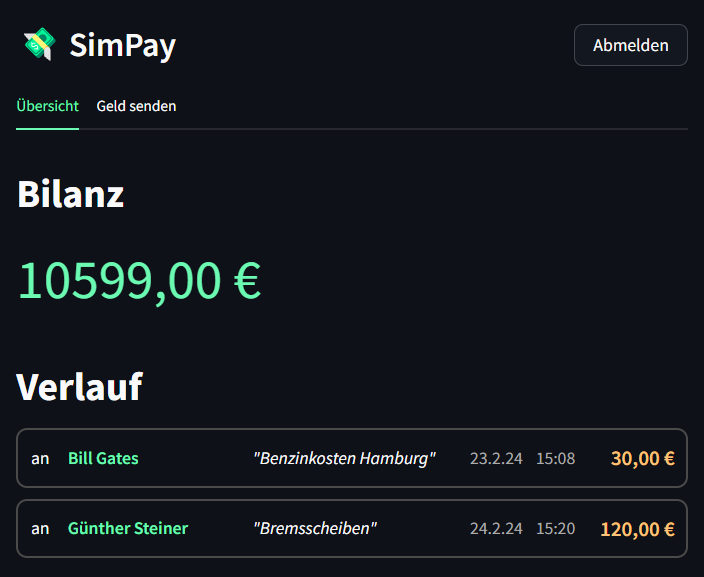
\includegraphics[width=.95\linewidth]{figures/impl/simpay_bilanz.png}
      \caption{Übersicht}
    %   \label{fig: blue totp app screenshot nicht verbunden}
    \end{subfigure}%
    \begin{subfigure}{.5\textwidth}
      \centering
      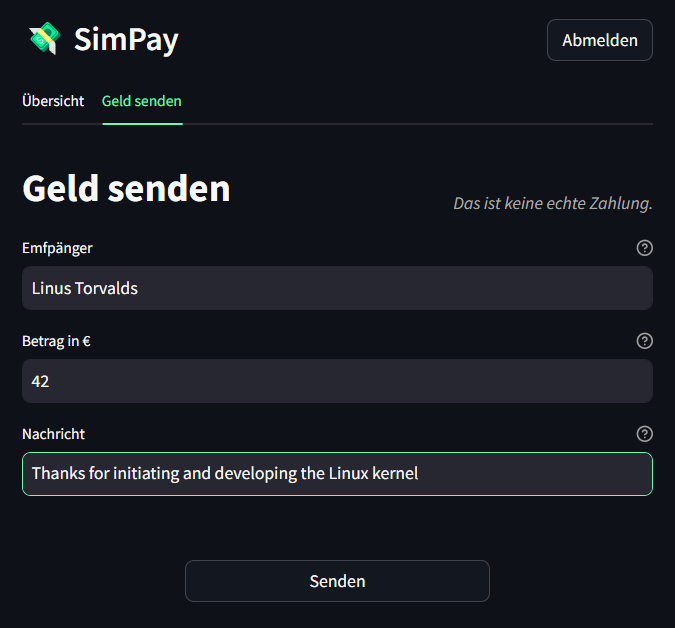
\includegraphics[width=.95\linewidth]{figures/impl/simpay_send.png}
      \caption{Überweisung}
    %   \label{fig: blue totp app screenshot verbunden}
    \end{subfigure}
    \caption[Website des fiktiven Dienstes Simpay]{Website des fiktiven Dienstes Simpay}
    \label{fig: simpay}
\end{figure}
\\\\
Der Webdienst wurde mit Streamlit\footnote{\href{https://streamlit.io/}{https://streamlit.io/}} (Python) als Frontend bzw. Host-Framework und 
einem eigens erstellten User Management und Logging entwickelt. Die Software wurde 
in einem Docker-Container auf einem Server des Instituts für Informatik der TU 
Bergakademie Freiberg gehostet. Die Verbindung zur Website wurde durch HTTPS 
gesichert. Die Passwörter der Teilnehmer werden mit der \textit{Password-Based Key 
Derivation Function 2} unter Verwendung des SHA256-Algorithmus, einer 
Iterationsanzahl von $700.000$ und einem 16 Byte langen Salt gehasht und 
gespeichert.

\newpage
\section{Studie}
    \label{sec: studie}
    Im Rahmen dieser Arbeit wurde eine Studie an der Technischen Universität 
Bergakademie Freiberg durchgeführt. Das Ziel der 
Studie ist die Untersuchung eines neuen Verfahrens für zeitbasierte 
Einmalpasswörter. Es sollte ermittelt werden, ob dieses Verfahren in seiner 
Anwendung potentiell schneller und nutzerfreundlicher als das gewöhnliche 
Verfahren für zeitbasierte Einmalpasswörter ist. Die Ethikkommission der Universität 
der Bundeswehr München hat die Studienskizze geprüft und der Durchführung zugestimmt.
\\\\
Die Forschungsfragen und Hypothesen wurden bereits in Kap. \ref{sec: forschungsansatz} vorgestellt.
\\\\
Im weiteren Verlauf dieses Kapitels wird die Studie vorgestellt. Es wird das 
Studiendesign, demographische Daten und Vorkenntnisse der Teilnehmer, der 
Apparat sowie der Ablauf der Studie präsentiert.

    \subsection{Studiendesign}
        \label{sec: studie studiendesign}
        Die Studie findet in Einzelsitzungen statt und beginnt mit einer Einführung zur 
Einrichtung des neuen Verfahrens. Am Folgetag beginnt die 6-tägige 
Nutzungsphase, in der die Probanden sich täglich bei einem Webdienst anmelden 
und mit dem neuen Verfahren als zweiten Faktor authentisieren. Auf der Website 
selbst schließen sie eine kleine Aufgabe ab, um dem gesamten Prozess eine Bedeutung zu vermitteln, anstatt sich grundlos irgendwo anzumelden. Am Ende der Nutzungsphase nehmen sie am abschließenden Meeting teil, 
um ihre Erfahrungen und Ansichten zu teilen.
\\\\
Der Fokus der Studie liegt auf der grundlegenden Untersuchung des Prototyps. Für den Vergleich zwischen Prototyp und traditionellen TOTP werden in der Abschlussveranstaltung die Fragebögen SUS bzw. UEQ genutzt. Hier kann man das zu bewertende System (Prototyp oder traditionelles TOTP) als unabhängige Variable sehen. Einmal bewerten die Probanden die Authentisierung bzgl. des traditionellen TOTP-Verfahrens und einmal bzgl. Blue TOTP.
\\\\
Die abhängigen Variablen sind folgende:
\begin{itemize}
    \item [(i)] Benötigte Zeit zur Einrichtung des neuen Verfahrens
    \item [(ii)] Nutzerfreundlichkeit, bemessen anhand der Fragebögen System Usability Scale (SUS) und User Experience Questionnaire (UEQ) für die Einrichtung des neuen Verfahrens
    \item [(iii)] Benötigte Zeit für die Authentisierung mit dem neuen Verfahren beim Webdienst pro Tag
    \item [(iv)] Nutzerfreundlichkeit, bemessen anhand der Fragebögen SUS und UEQ für die Authentisierung mit dem neuen Verfahren beim Webdienst
    \item [(v)] Nutzerfreundlichkeit, bemessen anhand der Fragebögen SUS und UEQ für die Authentisierung mit dem gewöhnlichen Verfahren beruhend auf der Erfahrung des Probanden
\end{itemize}
Variable (i) wird in der Einführungsveranstaltung per Stoppuhr gemessen und 
beginnt, sobald sich der Proband erstmals beim Webdienst angemeldet hat und 
direkt zur Einrichtung der Zwei-Faktor-Authentisierung (2FA) gezwungen wird. Das 
heißt, er sieht den zu scannenden QR-Code und das Eingabeelement für das initiale 
TOTP. 
Die Messung wird gestoppt, sobald der Proband das initiale TOTP beim Webdienst eingegeben hat. Den Teilnehmern 
wird nicht kommuniziert, dass ihre Zeit gemessen wird, damit sie möglichst 
natürlich und ohne Druck agieren.
\\\\
Variable (ii) sind die Ergebnisse aus den Fragebögen SUS und UEQ. 
\\\\
Variable (iii) bezieht sich auf die 6-tägige Nutzungsphase und wird vom 
Webserver gemessen. Die Messung beginnt, sobald der Proband beim Webdienst den 
Benutzernamen und das Passwort eingegeben hat und nun das TOTP eingeben muss. 
Wenn der Webdienst das TOTP erhalten hat, wird die Messung gestoppt. Werte von 
fehlgeschlagenen Authentisierungen werden nicht berücksichtigt. Den Teilnehmern 
wird nicht kommuniziert, dass ihre Zeiten gemessen werden, damit sie wie bei der 
Einrichtung möglichst natürlich und ohne Druck agieren.
\\\\
Die Variablen (iv) und (v) sind die Ergebnisse aus den Fragebögen SUS und UEQ 
jeweils für das neue und das gewöhnliche Verfahren. Sie werden direkt zu Beginn 
der Abschlussveranstaltung dem Probanden vorgelegt.

    \subsection{Probanden}
        \label{sec: studie probanden}
        An der TU Bergakademie Freiberg wurde öffentlich die Studie über die tägliche 
Rundmail beworben. Voraussetzung für die Teilnehmer war, dass sie bereits eine 
TOTP-App genutzt haben. D.h. sie sollten Kenntnis darüber haben, wie man das 
gewöhnliche TOTP-Verfahren einrichtet und bei der 2FA benutzt. Dies ist 
notwendig, damit sie das neue mit dem gewöhnlichen Verfahren vergleichen 
können. Des Weiteren müssen sie über ein Smartphone mit Android 10.0 oder höher 
verfügen sowie über einen Bluetooth-fähigen Computer mit Windows 10 oder 11. 
Eine weitere Beschränkung war, dass die Studie nur auf deutsch durchgeführt 
wurde, da die Benutzeroberfläche der Softwarekomponenten sowie die gesamten 
Unterlagen und Fragebögen zur Studie nur in deutsch verfasst sind.
Demographischen Einschränkungen bei der Auswahl der Teilnehmer bedarf es nicht.
Für die Teilnahme an der Studie hatten die Probanden einen Zeitaufwand von ca. 
2-3h und erhielten für die gesamte Studie eine Vergütung von 40 Euro.
\\\\
Insgesamt haben 11 Personen teilgenommen, davon 6 weibliche und 5 männliche. 
Rund 73\% der Teilnehmer gehören der Altersgruppe von 20-30 Jahren an. Die 
meisten Teilnehmer sind Studenten. Alle Teilnehmer besitzen mindestens das Abitur o.ä. als höchsten schulichen Abschluss.
\\\\
Bezüglich der Vorerfahrung mit TOTPs wurden die Teilnehmer ebenfalls befragt. 
Durchschnittlich haben sie 2 Dienste genutzt (jeder mind. einen), bei denen sie 
TOTPs als zweiten Faktor nutzen. Vier Probanden gaben an, TOTPs nur 1-3 mal pro Monat zu 
nutzen, während sechs angaben es 2 mal pro Woche oder häufiger zu nutzen. Bei der 
Frage, ob sie sich an die Einrichtung des TOTP-Verfahrens erinnern, konnten nur 
wenige beschreiben, dass man einen QR-Code scannt und anschließend das erste 
TOTP eingibt. Nachdem es ihnen erklärt wurde, erinnerten sich alle Teilnehmer wieder an 
die Einrichtung und sagten aus, dass sie die Einrichtung nicht 
als schwierig empfanden. Zwei Teilnehmer gaben an, noch nie aktiv eine Browser-Extension genutzt zu haben.

    \subsection{Apparat}
        \label{sec: studie apparat}
        Jeder Proband benötigt für die Studie einen Bluetooth-fähigen Computer und ein 
Bluetooth-fähiges Android-Smartphone. Idealerweise sollten die Geräte Eigentum der 
Probanden sein, da man für gewöhnlich am besten mit seinen eigenen Geräten und 
deren Konfigurationen zurechtkommt. Zur Einführung und zur selbstständigen 
Nutzungsphase benötigen die Probanden einen Internetzugang, um den Webdienst 
aufzurufen. Um die nötigen Softwarekomponenten zu installieren, sollten sie 
Administratorrechte besitzen. Die Softwarekomponenten setzen sich zusammen aus 
der Smartphone-App (Speichern und Übertragen der TOTPs) sowie der Browser 
Extension (für Chrome) und einer Hintergrundanwendung (zum Empfangen und 
automatischen Eintragen des TOTPs). Details sind in Kap. \ref{sec: implementierung} zu finden.
\\\\
Ein weiterer Bestandteil des Experiments ist der Webdienst, der zuverlässig und 
jederzeit erreichbar sein sollte. Hier werden unter anderem die Anmeldedaten und 
Logging-Daten der Probanden gespeichert. Mithilfe der Zeitstempel in den 
Logging-Daten wird die Dauer jeder Authentisierung gemessen. Der Webdienst 
unterstützt die Anmeldung mit Benutzername und Passwort und verlangt nach dem 
ersten Login die Einrichtung der 2FA mit zeitbasierten Einmalpasswörtern. Dieser 
Einrichtungsprozess ist so aufgebaut wie jeder Einrichtungsprozess von TOTPs: 
QR-Code anzeigen, kurze Anweisungen, was der Nutzer tun muss, und ein Eingabefeld 
für das initale TOTP. Der Webdienst selbst bietet dem Probanden die Möglichkeit, 
eine fiktive Aufgabe zu erledigen, die bestenfalls einen sicherheitskritischen 
Kontext wie Finanzen hat, damit der Proband die 2FA zumindest in der Fiktion als 
sinnvoll erachtet.
\\\\
Darüber hinaus werden Materialien wie die standardisierten Fragebögen User 
Experience Questionnaire (UEQ) \autocite{Schrepp} und System Usability Scale (SUS)
\autocite{Brooke} benötigt. Beide Fragebögen werden insgesamt dreimal benötigt: 
nach der Einrichtung des neuen Verfahrens und zu Beginn der 
Abschlussveranstaltung für das neue sowie das gewöhnliche Verfahren.
\\\\
Zudem wurden den Probanden Fragen in einem Interview gestellt: einmal nach der 
Einrichtung des neuen Verfahrens und in der Abschlussveranstaltung. Der 
Fragenkatalog ist im Anhang \ref{anh: interview einrichtung} und \ref{anh: interview authentisierung} einzusehen. 

\subsection{Entscheidung für SUS und UEQ}
Es existieren verschiedene standardisierte Fragebögen, um zu ermitteln, wie 
Nutzer ihre Erfahrung mit einem System bewerten und inwiefern sie es als 
nutzerfreundlich erachten. Folgend wird begründet, wieso sich für UEQ und SUS entschieden wurde. 
\\\\
Ein sehr bekannter Fragebogen zur Nutzerfreundlichkeit / Benutzbarkeit ist die 
System Usability Scale (SUS) \autocite{Brooke}. Sie besteht aus 10 
standardisierten Aussagen über das verwendete System. Wobei ein Teilnehmer mit 
Hilfe einer 5-stufigen Skala zu jeder Aussage seine Zustimmung oder seinen 
Widerspruch äußert. Aus den Antworten wird eine Punktzahl berechnet, die dann 
eine Aussage über die Nutzerfreundlichkeit eines Systems treffen soll. Das 
Ergebnis liegt immer in einem Bereich von 0 bis einschließlich 100 Punkte, wobei 
100 Punkte für die bestmögliche und 0 Punkte für die schlechtestmögliche 
Nutzerfreundlichkeit stehen. Als durchschnittliche Bewertung werden 68 Punkte 
angesehen und die prozentuale Wertigkeit der Punkte verläuft nicht linear, sondern als 
S-Kurve \autocites{Sauro}[zitiert nach][]{BrookeRetro}. Die SUS eignet sich, um zwischen verschiedenen 
Systemen zu vergleichen, da ihre zu bewertenden Aussagen allgemein verfasst sind.
Prinzipiell kann der Vergleich zu den Studienergebnissen von Reese et al. \autocite{Reese} angestellt werden. Am Ende des SUS-Fragebogens wird eine 11. Frage gestellt, die separat ausgewertet wird. Hier geben die Probanden auf einer $7$-stufigen Skala an, wie nutzerfreundlich sie das System insgesamt bewerten \autocite{SUS11}. Die Stufen werden mit Aussagen wie \glqq Das Schlechteste, was man sich vorstellen kann\grqq{} über \glqq Ok\grqq{} bis hin zu \glqq Das Beste, was man sich vorstellen kann\grqq{} versehen. Diese Aussagen werden entsprechend der Erkenntnisse von \textcite{SUS11} einer SUS-Punktzahl zugeordnet. Mithilfe dieser Ergebnisse wird verglichen, ob die tatsächlichen SUS-Berwertungen der empfundenen Nutzerfreundlichkeit annährend entsprechen.
\\\\
Des Weiteren wird der User Experience Questionnaire (UEQ) Fragebogen genutzt. Er 
dient dazu, ein System bzgl. der Nutzerfreundlichkeit und 
Nutzererfahrung zu bewerten. Der UEQ besteht aus 26 Begriffspaaren, wobei sich 
jedes Paar aus jeweils zwei gegensätzlichen Adjektiven zusammensetzt. Mit einer 
7-stufigen Skala muss der Proband für jedes Begriffspaar seine Zustimmung zu 
einem der Begriffe in Bezug auf das System äußern. Setzt er ein Kreuz in der 
Mitte der Skala, stimmt er für beide Begriffe gleichermaßen. Diese 26 Paare 
werden unterteilt in sechs Skalen \autocite[2]{Schrepp}:
\begin{itemize}
    \item Attraktivität: Gesamteindruck über das System, mögen Nutzer das System oder nicht?
    \item Durchschaubarkeit: Gewöhnt man sich leicht an das System, ist es leicht zu erlernen?
    \item Effizienz: Kann die Aufgabe ohne unnötigen Aufwand gelöst werden?
    \item Steuerbarkeit: Beherrscht der Nutzer das System?
    \item Stimulation: Ist die Nutzung des Systems spannend und motivierend?
    \item Originalität: Ist das System innovativ und kreativ? Weckt es das Interesse?
\end{itemize}
Somit wird analysiert, ob in einer Skala Stärken oder Defizite vorliegen. Dies kann 
man sowohl für ein einzelnes System (hier die Einrichtung von Blue TOTP) als auch zum Vergleich 
zweier Systeme nutzen (hier das traditionelle TOTP-Verfahren gegenüber Blue TOTP).

    \subsection{Ablauf}
        \label{sec: studie prozedur}
        Bevor interessierte Personen zur Studie zugelassen wurden, mussten sie eine 
Online-Umfrage mit vier Fragen durchlaufen. Dabei wurde erfragt, ob sie 
Vorerfahrung mit zeitbasierten Einmalpasswörtern und einer entsprechenden 
Authenticator App haben. Außerdem wurde überprüft, ob ihr Smartphone eine 
gewisse Bluetooth-Funktion unterstützt (siehe Kap. \ref{sec: implementierung architektur}). Am Ende 
wurden sie noch gebeten, den Chrome-Browser zu installieren. Waren alle 
Voraussetzungen erfüllt, wurden sie zur Einführung eingeladen. Die Einführung 
und der Abschluss fanden in Einzelsitzungen statt. So konnten die Probanden 
bei der Einrichtung besser beobachtet werden und der Versuchsleiter konnte jedem 
Probanden mit ungeteilter Aufmerksamkeit behilflich sein. Da es Einzelsitzungen waren, war es nicht möglich, dass die Antworten eines Probanden durch 
andere Probanden beeinflusst wird.

        \subsubsection{Einführung}
            \label{sec: studie prozedur einfuerung}
            Zu Beginn der Einführungsveranstaltung haben die Teilnehmer die 
Teilnehmerinformation gelesen, falls noch nicht geschehen, und füllten 
anschließend die Einverständniserklärung aus. Danach wurden sie noch einmal 
kurz über den Ablauf der gesamten Studie aufgeklärt. Dabei wurden sie bestärkt, 
dass sie nichts falsch machen können und bei Problemen jederzeit den 
Versuchsleiter ansprechen sollen. Dann wurde mit der Aufnahme der 
demographischen Daten sowie der Vorkenntnisse zu TOTPs begonnen. Dies geschah 
teilweise automatisiert mit LimeSurvey\footnote{\href{https://www.limesurvey.org/}{https://www.limesurvey.org/}}, teilweise als Interview. Die Teilnehmer wurden 
gefragt, ob ihnen das Prinzip der 2FA bekannt ist.
\\\\
Im nächsten Abschnitt installierten die Teilnehmer gemeinsam mit dem 
Versuchsleiter die notwendigen Programme: ggf. Chrome, die Browser-Extension 
und deren Hintergrundanwendung sowie die Smartphone-App. Da es sich bei der 
Implementierung um einen Prototyp handelt, sind die App, die Extension und 
deren Hintergrundanwendung nicht in den offiziellen Software Stores (Google 
Play Store, Chrome Web Store, Microsoft Store) veröffentlicht und auch nicht 
signiert. D.h. die Teilnehmer mussten für ihr Android-Gerät die App über eine  
\glqq Android Package Kit\grqq-Datei (APK) installieren und fremde Quellen 
zulassen. Für Windows war es ähnlich. Die Extension musste über den 
Entwicklermodus von Chrome installiert werden. Dadurch war der gesamte 
Installationsprozess verhältnismäßig sehr aufwändig und daher kein Bestandteil 
der Beurteilung der Probanden. Nach der Installation haben die Probanden die 
Extension und App kurz geöffnet, um die Onboardings zu überspringen, da diese 
gerade durchgeführt wurden. Daraufhin haben sich die Probanden beim Webdienst 
registriert. Ab diesem Punkt wurde erwähnt, dass die Probanden alles vergessen 
sollten, was sie bis jetzt durchlaufen haben. Somit sollte sichergestellt werden, dass anschließend nur die Einrichtung der 2FA mit Blue TOTP bewertet wird und nicht die Installation der Programme.
\\\\
Den Probanden wurde erklärt, dass sie nun mit der Einrichtung des neuen 
Authentisierungsverfahrens beginnen werden, wobei sie die eben installierten 
Programme (App und Extension) nutzen sollen. Ebenso wurde ihnen gesagt, dass sie diesen Prozess 
anschließend bewerten werden. Die Probanden haben sich beim Webdienst 
angemeldet und eine Anleitung zur Einrichtung der Zwei-Faktor-Authentisierung 
gesehen. 
Zu diesem Zeitpunkt startet der Versuchsleiter unauffällig die Stoppuhr. Dann 
mussten die Probanden den zusätzlichen Anweisungen in der App und der Browser 
Extension folgen. Nur bei großen Schwierigkeiten schritt der Versuchsleiter 
ein, um sie auf den richtigen Pfad zu führen. Während der Einrichtung wurden 
alle Probleme oder Auffälligkeiten notiert. Mit erfolgreichem Abschluss der 
Einrichtung wurde die Stoppuhr angehalten und die Zeit notiert.
\\\\
Anschließend haben die Teilnehmer UEQ und SUS bzgl. der Einrichtung  
ausgefüllt. Danach wurde das Interview mit ihnen geführt (siehe Anhang \ref {anh: interview einrichtung}).
Das Interview dient dazu, die so eben erlebten Erfahrungen, Gedanken und Ideen 
des Probanden zu äußern. Bis zum Ende des Interviews (also auch nicht bei SUS und 
UEQ) wusste der Proband noch nicht, worin sich das eben untersuchte Verfahren vom 
gewöhnlichen Verfahren unterscheidet. Denn der Proband hat sich bis zu diesem 
Zeitpunkt noch nicht mithilfe des neuen Verfahrens authentisiert. Somit sind 
seine Aussagen nicht davon beeinflusst, wie gut oder schlecht das System in 
seiner eigentlichen Nutzung (der 2FA) funktioniert.
\\\\
Am Ende hat der Proband noch einen Testlauf für die kommenden Tage 
durchgeführt und so die eigentliche Nutzung des neuen Verfahrens kennengelernt. D.h. er hat sich zunächst beim Webdienst erneut angemeldet. 
Daraufhin hat er mit Blue TOTP erstmals das Einmalpasswort automatisch in die 
Website übertragen lassen. Dann hat er auf der Website noch eine fiktive 
Überweisung getätigt.
Zum Schluss wurden noch Formalitäten wie der Termin zum Abschlussmeeting geklärt 
und der erste Teil der Vergütung in Höhe von 15 Euro ausgezahlt. Die Einführung 
dauerte i.d.R. eine Stunde.

        \subsubsection{6-tägige Nutzungsphase}
            \label{sec: studie prozedur phase}
            Nun hat der Proband die Aufgabe, sich täglich für sechs Tage in Folge beim 
Webdienst anzumelden und eine fiktive Überweisung zu tätigen. Dies geschah von 
zu Hause aus oder unterwegs. Dazu muss er nach der Anmeldung mit Benutzername 
und Passwort immer den zweiten Faktor mit dem neuen Verfahren automatisch in 
die Website übertragen lassen. Um den Probanden nicht unter Druck zu setzen, 
wurde nicht kommuniziert, dass die benötigte Zeit zur Authentisierung gemessen 
wurde. Immer um 1:00 Uhr morgens wurde den Teilnehmern ihre Aufgabe per E-Mail 
zugesendet. Wer bis 19:00 seine Aufgabe noch nicht erledigt hatte, bekam eine 
Erinnerungsmail. Wenn ein Teilnehmer seine Aufgabe nicht erfüllt hat, sollte er 
am Folgetag einmal früh und dann abends die Aufgabe erledigen.

        \subsubsection{Abschluss}
            \label{sec: studie prozedur abschluss}
            Zu Beginn der Abschlussveranstaltung füllten die Probanden erst SUS und UEQ zum 
gewöhnlichen TOTP-Verfahren aus und dann SUS und UEQ zum neuen TOTP-Verfahren. 
Vorher wurden sie mündlich und schriftlich ausdrücklich darauf hingewiesen, 
dass es sich dabei um die Beurteilung des Anmeldungsprozesses handelt unter 
Verwendung der gewöhnlichen TOTP-Apps bzw. die App und Browser-Extension für 
das neue Verfahren. Das Design und die Funktionalität der Website sollte dabei 
außen vor gelassen werden. Danach wurde ein Interview geführt, um wieder die 
Erfahrungen, Gedanken und Ideen der Probanden festzuhalten. Zum 
Schluss wurde den Probanden für ihre Teilnahme an der Studie gedankt und die 
restliche Vergütung von 25 Euro ausgezahlt.
        
\newpage
\section{Ergebnisse der Studie}
    \label{sec: ergebnisse studie}
    Zunächst werden einige Grundlagen bzgl. der Zwei-Faktor-Authentisierung  geklärt. 
Dabei werden gängige Verfahren sowie deren Stärken und Schwächen bzgl. der Sicherheit 
und Nutzerfreundlichkeit betrachtet. Es wird die Problematik des Phishings vorgestellt 
und anschließend Passkeys sowie verwandte Arbeiten besprochen. 

    \subsection{Einrichtung}
        \label{sec: ergebnisse studie einrichtung}
        Die Einrichtung fand in der Einführungsveranstaltung statt und umfasste nur das
Einrichten der Zwei-Faktor-Authentisierung mit Hilfe des Prototypen \glqq Blue 
TOTP\grqq{}. Die Installation der Software ist kein Bestandteil dieser Ergebnisse.


        \subsubsection{Einrichtungszeit}
            \label{sec: ergebnisse studie einrichtungszeit}
            Die Einrichtungszeit ist die Zeit, die benötigt wird, um die 
Zwei-Faktor-Authentisierung beim Webdienst einzurichten. Die Messung 
beginnt, sobald der Proband auf der Website die Anweisungen zur 
Einrichtung sieht (QR-Code scannen, initiales TOTP eingeben). Nach der 
Eingabe und Bestätigung des initialen TOTPs wird die Messung beendet.
\\\\
Bei den 11 Probanden wurde jeweils ein Wert für die Einrichtungszeit 
gemessen. Ein Boxplot sowie die Verteilung der Werte ist in Abb. \ref
{fig: studie setup time boxplot} bzw. Abb. \ref{fig: studie setup time dist} dargestellt. Auffällig ist, dass ungefähr die Hälfte der Einrichtungen nicht länger 
als ca. 200~s dauerte, während die verbleibenden Einrichtung länger als 
ca. 290~s dauerten. Durchschnittlich haben die Probanden dem Median 
zufolge 177~s und dem Mittelwert nach 228~s benötigt (siehe Anhang \ref
{anh: studie ergebnisse setup} Tab. \ref{tab: studie setup time}). Die Spannweite 
der Zeiten reicht von 84~s bis zu 348~s.
\newpage
\begin{figure}[h]
    \begin{minipage}[b]{.42\textwidth}
        \centering
        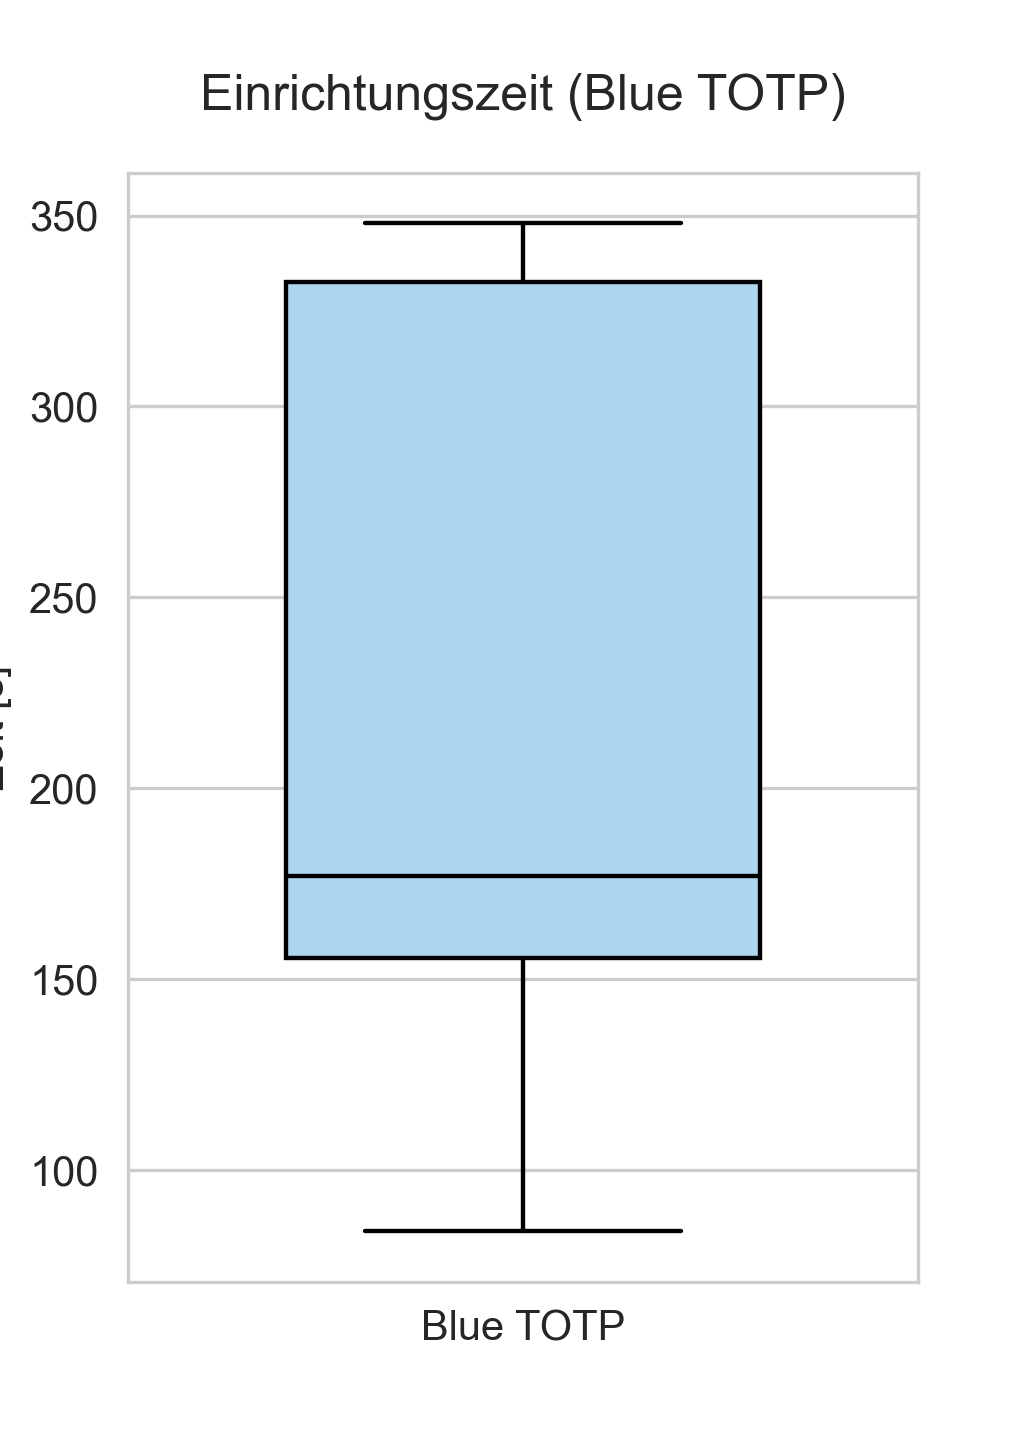
\includegraphics[width=0.8\linewidth]{data_processing/timings/results/setup_timings_boxplot.png}
        \caption[Einrichtungszeit von Blue TOTP]{Einrichtungszeit von Blue TOTP}
        \label{fig: studie setup time boxplot}
    \end{minipage}
    \hfill
    \begin{minipage}[b]{.54\textwidth}
        \centering
        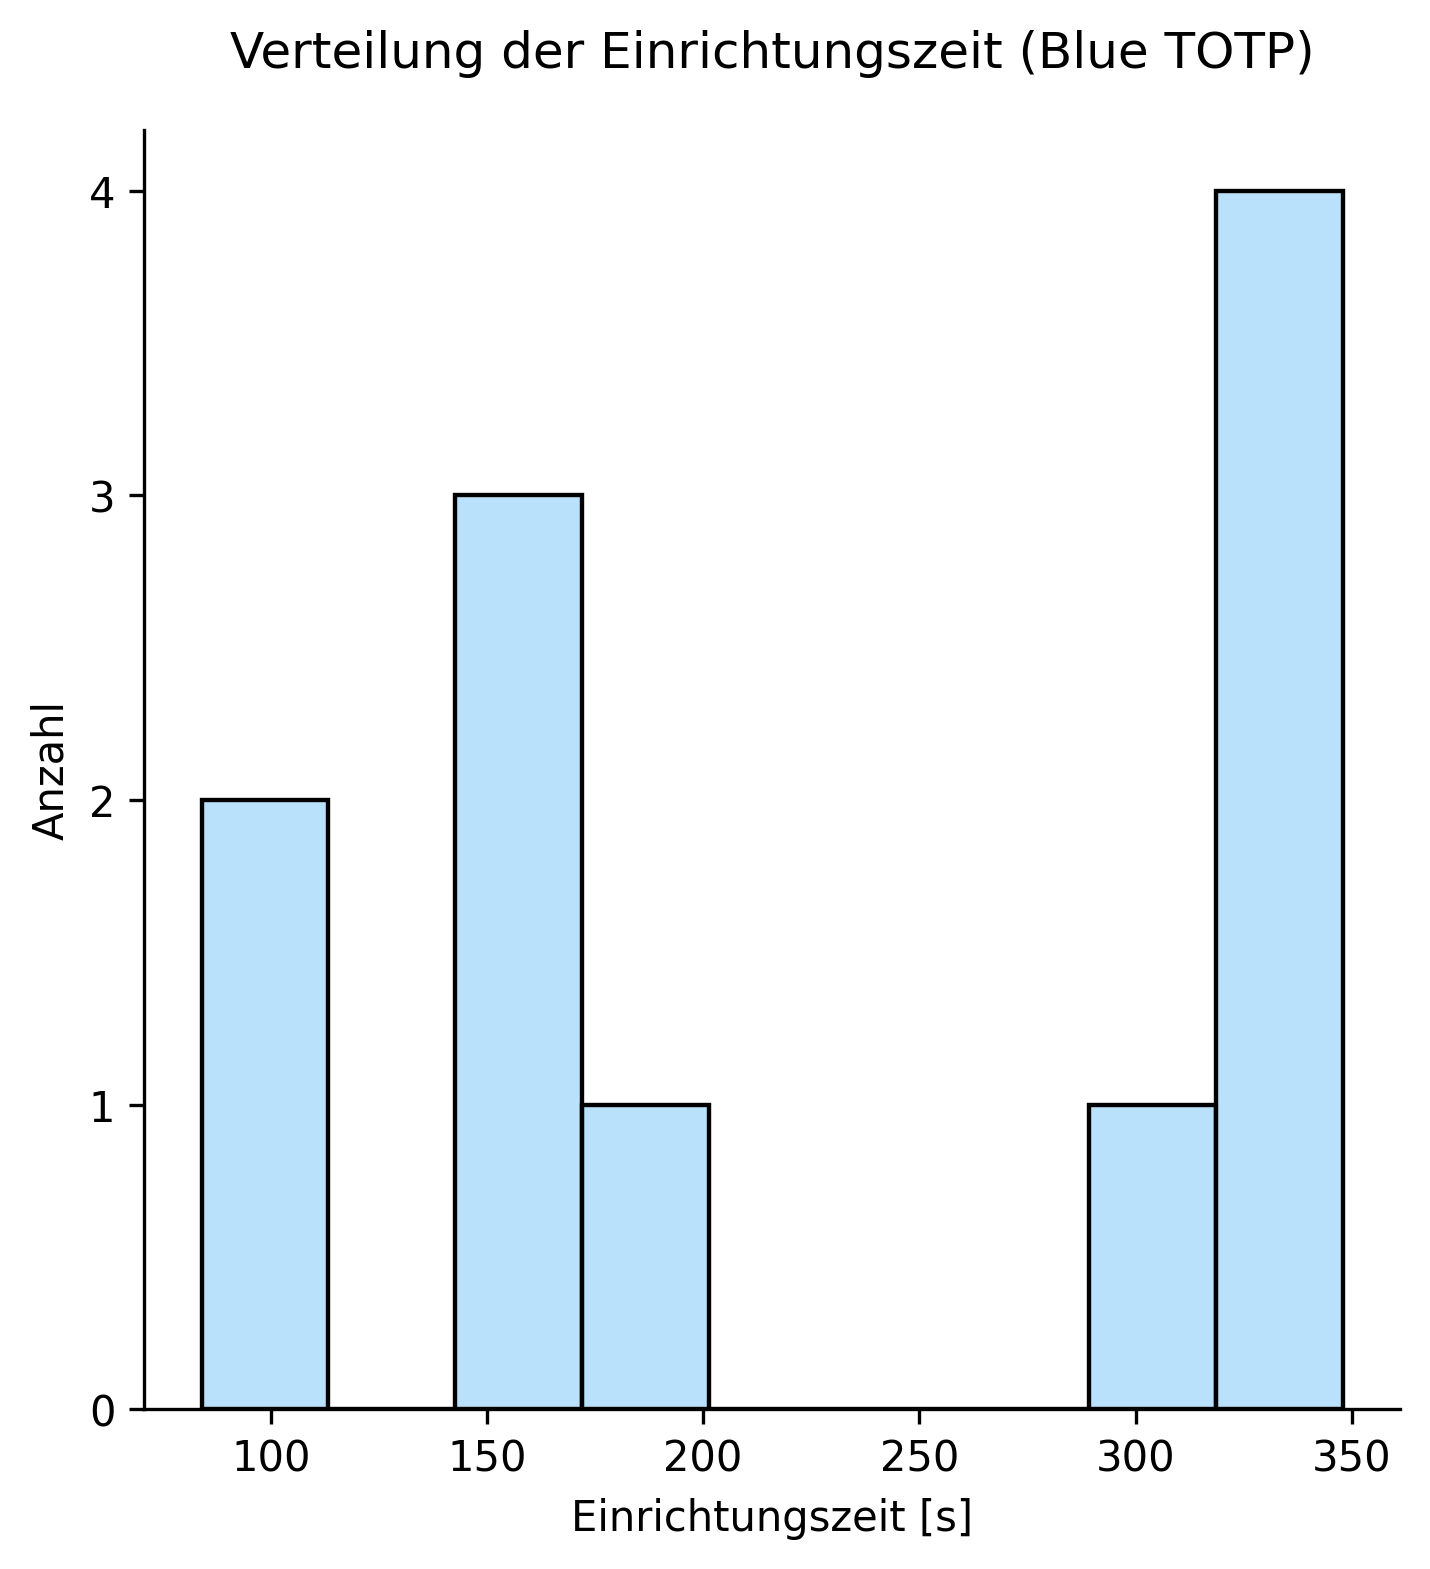
\includegraphics[width=0.78\linewidth]{data_processing/timings/results/distribution_of_setup_data.png}
        \caption[Verteilung der Einrichtungszeit von Blue TOTP]{Verteilung der Einrichtungszeit von Blue TOTP}
        \label{fig: studie setup time dist}
    \end{minipage}
\end{figure}


        \subsubsection{User Experience Questionaire}
            \label{sec: ergebnisse studie ueq}
            Beim Ausfüllen des UEQ sollten sich die Probanden nur auf den 
Einrichtungsprozess an sich beziehen und auf die Handhabung der 
Blue TOTP App sowie der Blue TOTP Extension. Der Einfluss der 
Website sollte außen vor gelassen werden.
\\\\
Die Verteilung der Antworten zu den Gegensatzpaaren des UEQ sind in Abb. \ref{fig: studie setup ueq dist} zu sehen.
\begin{figure}[h]
    \centering
    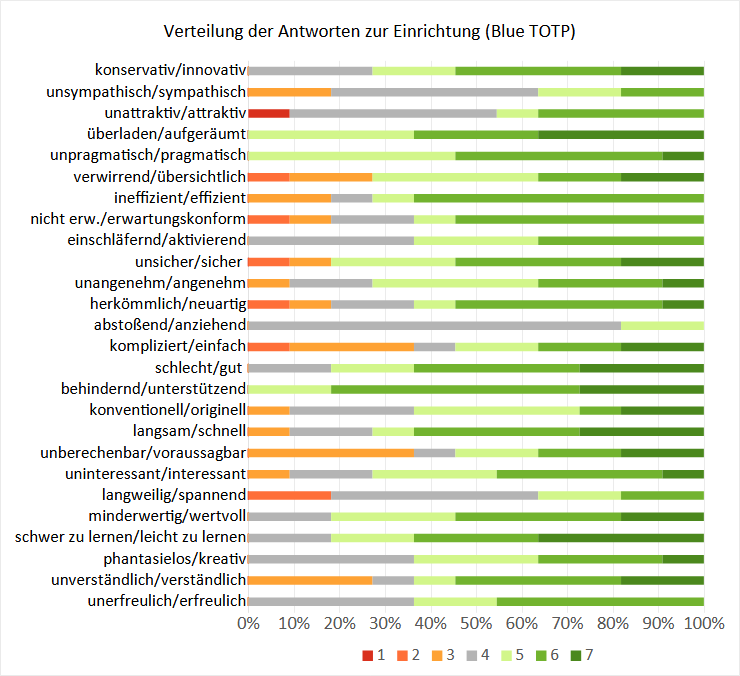
\includegraphics[width=.9\linewidth]{data_processing/questionaires/results/figures_from_excel/setup_ueq_distribution.png}
    \caption[Verteilung der Antworten zum UEQ (Einrichtung Blue TOTP)]{Verteilung der Antworten zum UEQ (Einrichtung Blue TOTP). Die Tendenzen: 1 stärkste Tendenz zum negativen Begriff, 4 neutral, 7 stärkste Tendenz zum positiven Begriff}
    \label{fig: studie setup ueq dist}
\end{figure}
Die Antworten tendieren überwiegend zu den positiven Begriffen 
der Begriffspaare, gefolgt von neutralen Antworten. Die am 
stärksten positiv ausgeprägten Begriffe sind \glqq unterstützend\grqq{} mit 
$\bar{x} = 2{,}1$ und \glqq aufgeräumt\grqq{} mit $\bar{x} = 2{,}0$ (vergl. Anhang 
\ref{anh: studie ergebnisse setup} Tab. \ref{tab: studie setup ueq item 
means}). Interessant  ist die starke Tendenz dahingehend, dass 
das System \glqq leicht zu lernen\grqq{} ($\bar{x} = 1{,}8$) sei, aber es 
dennoch als eher schlecht \glqq voraussagbar\grqq{} ($\bar{x} = 0{,}7$) 
wahrgenommen wird. Zusätzlich dazu überzeugt das System nicht 
sonderlich bzgl. des Paares \glqq einfach/kompliziert\grqq{} mit $\bar{x} = 0.6$.
Das Paar \glqq abstoßend/anziehend\grqq{} wurde beinahe vollständig 
neutral beantwortet, wobei die zwei nicht neutralen Antworten 
direkt an neutral liegen. Das ist ein Indiz dafür, dass die 
Probanden das Begriffspaar nicht mit dem System assoziieren 
können.
\\\\
Durch die Aufteilung der Gegensatzpaare zu ihrer zugehörigen 
Skala (vergl. \autocite[3]{Schrepp}) wurden die in Abb. 
\ref{fig: studie setup ueq overview} dargestellten Mittelwerte 
berechnet. 
\begin{figure}[h!]
    \centering
    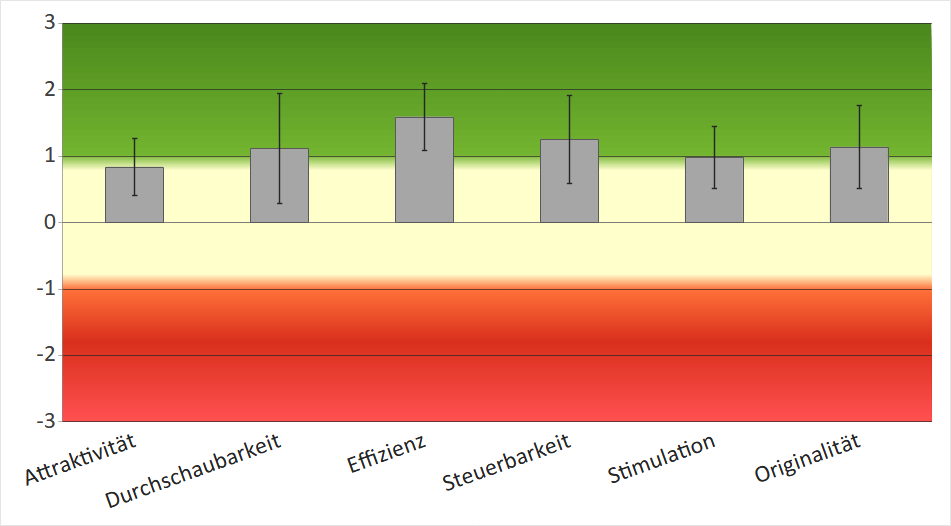
\includegraphics[width=.75\linewidth]{data_processing/questionaires/results/figures_from_excel/setup_ueq_overview.png}
    \caption[Mittelwerte der UEQ-Skalen zur Einrichtung von Blue TOTP]{Mittelwerte der UEQ-Skalen mit 95\%-Konfidenzintervallen zur Einrichtung von Blue TOTP. Farbliche Unterteilung in Bereiche: grün als positiv ($\ge 0.8$), gelb als neutral, rot als negativ ($\le 0.8$)}
    \label{fig: studie setup ueq overview}
\end{figure}
Es ist erkennbar, dass die Einrichtung mit Blue TOTP im Mittel 
bei der Skala Effizienz ($\bar{x} = 1{,}59$) die markanteste Stärke 
besitzt. Auch die Steuerbarkeit ($\bar{x} = 1{,}25$) liegt noch 
deutlich im positiven Bewertungsbereich (größer 0{,}8). Dagegen 
befindet sich die Attraktivität ($\bar{x} = 0{,}83$) auf der Grenze 
zwischen dem neutralen und positiven Bereich. Die verbleibenden 
Skalen Durchschaubarkeit ($\bar{x} = 1{,}11$), Stimulation ($\bar{x} 
= 0{,}98$) und Originalität ($\bar{x} = 1{,}14$) sind nahe über dieser 
Grenze.
\newpage
        
        \subsubsection{System Usability Scale}
            \label{sec: ergebnisse studie sus}
            Ebenso wie beim UEQ, sollten die Probanden sich auch beim SUS-Fragebogen nur 
auf den Einrichtungsprozess selbst beziehen und auf die Handhabung der Blue 
TOTP App sowie der Blue TOTP Extension.
\\\\
Die SUS-Bewertungen sind in Abb. \ref{fig: studie setup sus boxplot} zu sehen. 
\begin{figure}
    \centering
    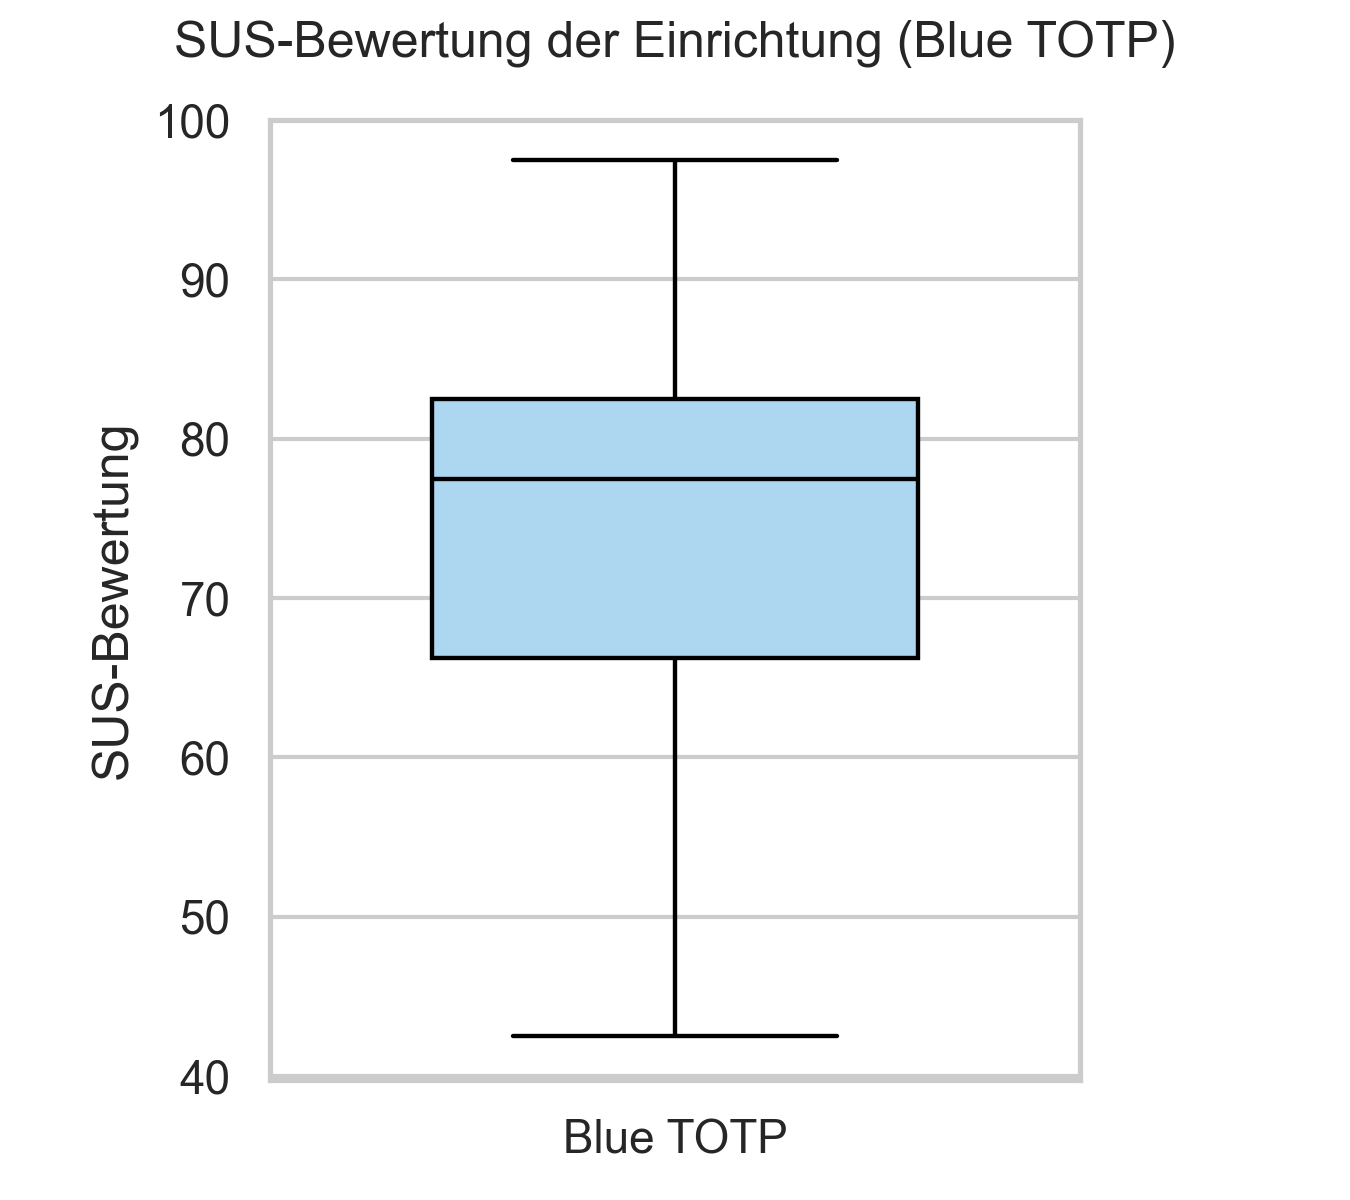
\includegraphics[width=.5\linewidth]{data_processing/questionaires/results/setup_sus_boxplot.png}
    \caption[SUS-Bewertung der Einrichtung von Blue TOTP]{SUS-Bewertung der Einrichtung von Blue TOTP}
    \label{fig: studie setup sus boxplot}
\end{figure}
Die schlechteste Bewertung erreichte ca. 43 Punkte, während die beste mit ca. 
98 Punkten nahe dem Maximum ist. Die Probanden haben die Einrichtung mit einem 
Median von 77.5 Punkten bewertet. Der Mittelwert liegt bei $75{,}8$ Punkten. 
Demnach liegt die Punktzahl über dem allgemeinen Vergleichswert von 68 Punkten.
\\\\
Zusätzlich wurde mit einer 7-stufigen Likert-Skala erfragt, wie nutzerfreundlich die Probanden das System insgesamt bewerten. Diese Werte werden mit einer zugehörigen SUS-Punktzahl gleichgesetzt \autocite{SUS11}. In Abb. \ref{fig: studie setup sus vs sus11} ist der Unterschied zwischen der empfundenen Nutzerfreundlichkeit und der eigentlichen SUS-Bewertung dargestellt.
\begin{figure}[h]
    \centering
    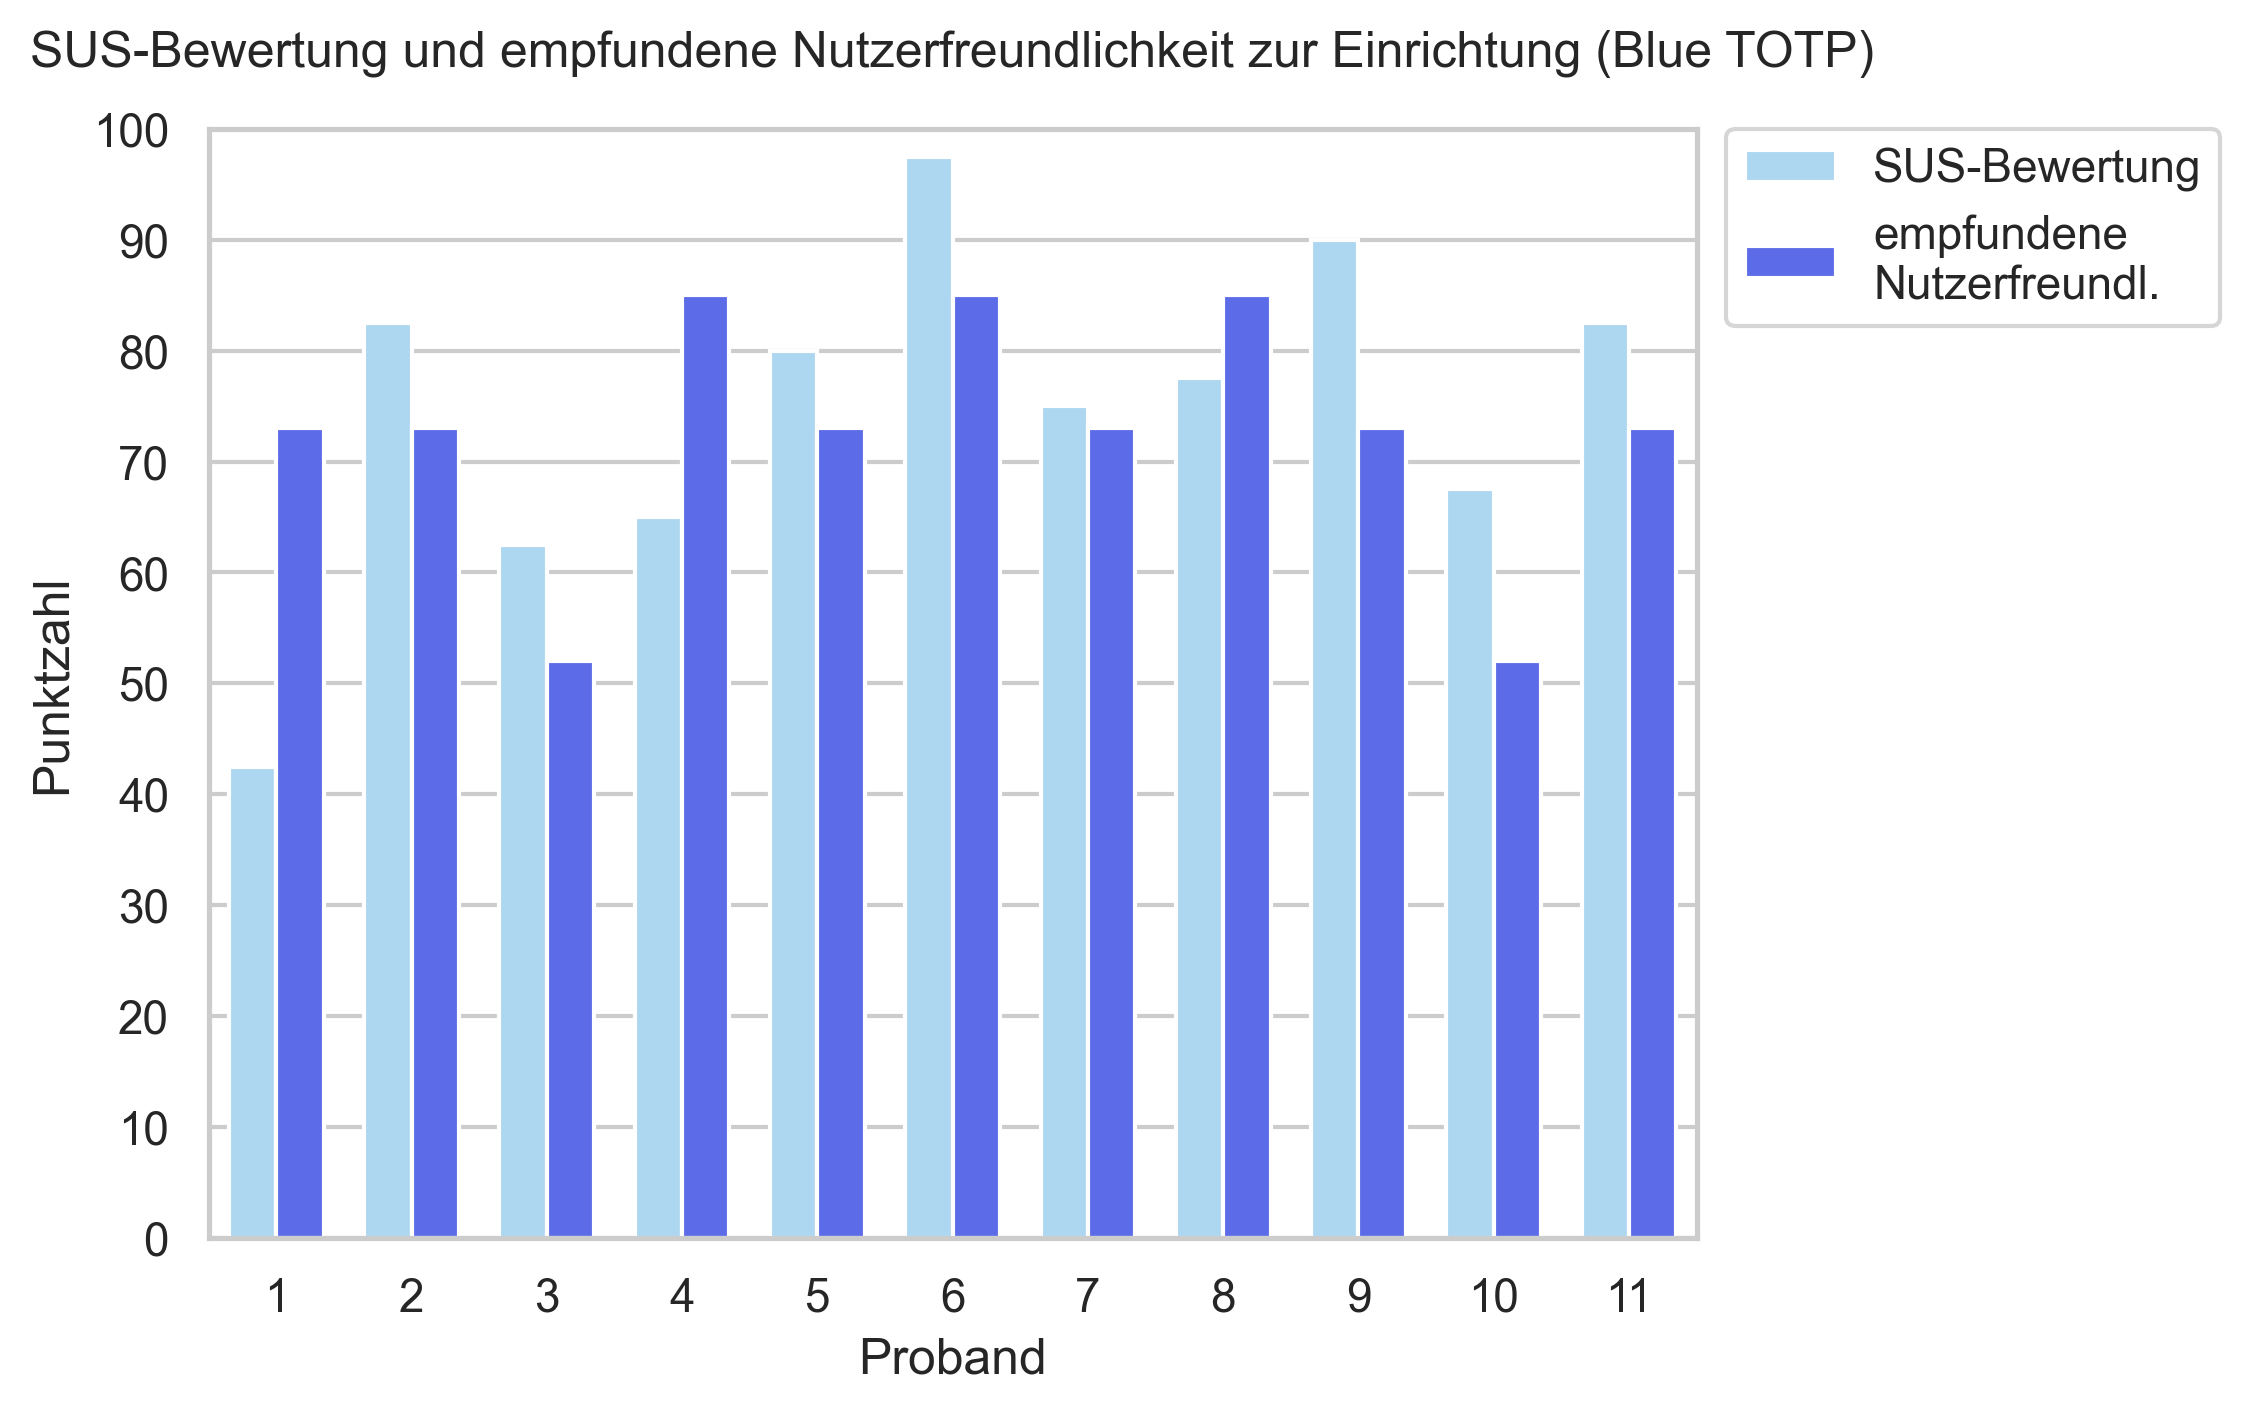
\includegraphics[width=.8\linewidth]{data_processing/questionaires/results/setup_sus_vs_sus11.png}
    \caption[SUS-Bewertung und empfundene Nutzerfreundlichkeit (Einrichtung Blue TOTP)]{SUS-Bewertung und empfundene Nutzerfreundlichkeit \autocite{SUS11} pro Proband zur Einrichtung von Blue TOTP}
    \label{fig: studie setup sus vs sus11}
\end{figure}
Die größte absolute Differenz hat Proband P1 mit ca. 30 Punkten, gefolgt von P4 
(20 Pkt.), P9 (17 Pkt.) und P10 (15 Pkt.). Die restlichen absoluten Differenzen 
schwanken zwischen 7 und 13 mit Ausnahme von P7 (2 Pkt.). Die 
Standardabweichung der absoluten Differenzen beträgt $7{,}7$ Punkte.
\\\\
\begin{table}[b]
    \centering
    \begin{center}
    \begin{tabular}{| l | c | c | c | c | c | c | c | c | c | c |}
        \hline
        \textbf{Aussage} & 1 & 2 & 3 & 4 & 5 & 6 & 7 & 8 & 9 & 10 \\
        \hline
        \textbf{Mittelwert} & $2{,}73$ & $3{,}18$ & $3{,}0$ & $2{,}82$ & $2{,}82$ & $3{,}27$ & $3{,}27$ & $3{,}27$ & $2{,}55$ & $3{,}0$ \\  
        \hline
    \end{tabular}
    \end{center}
    \caption[Durchschnittliche Bewertung pro Aussage des SUS (Einrichtung Blue TOTP)]{Durchschnittliche Bewertung pro Aussage des SUS (Einrichtung Blue TOTP)}
    \label{tab: studie setup sus mean per question}
\end{table}
Jeder Aussage im SUS-Fragebogen wird entsprechend der 5-stufigen Skala ein Wert 
von 0 bis 4 zugeordnet (0 sehr negativ behaftet, 2 neutral, 4 sehr positiv). 
Bildet man pro Aussage den Mittelwert über alle Probanden, erhält man die 
Ergebnisse in Tab. \ref{tab: studie setup sus mean per question}. Keine Aussage weist eine negativ behaftete Tendenz auf 
(kein Mittelwert kleiner 2). Den schlechtesten Durchschnitt bildet Aussage 9 
\glqq Ich habe mich bei der Nutzung des Systems sehr zuversichtlich gefühlt\grqq{} mit 
$\bar{x} = 2{,}55$. 
Besonders variieren die Werte bei Aussage 4 \glqq Ich glaube, ich würde die Hilfe 
einer technisch versierten Person benötigen, um das System benutzen zu können\grqq{}. 
Hier stimmten drei Probanden mit den Werten 1 oder 0 für die Richtigkeit der 
Aussage (also sie brauchen die Hilfe), während alle anderen mit den Werten 3 
oder 4 zum Ausdruck brachten, dass sie wenig bis keine Hilfe benötigen.

        \subsubsection{Beobachtungen}
            \label{sec: ergebnisse studie beobachtungen}
            Während die Probanden die Einrichtung durchgeführt haben, hat der Versuchsleiter sie dabei beobachtet und Auffälligkeiten protokolliert. Zu Beginn hat die Website immer den QR-Code und eine 
allgemeingültige Anleitung angezeigt, die auch für das normale TOTP-Verfahren 
funktioniert.
\\\\
Jeder Proband hat damit begonnen, den angezeigten QR-Code zu scannen. Ungefähr 
die Hälfte hat versucht, den QR-Code mit der Scan-Funktion von Android zu 
scannen, anstatt dies direkt über die App zu tun. Allerdings unterstützt die 
Blue TOTP App es nicht, dass man sie über die Scan-Funktion von Android öffnet.
Einige wussten nicht, wie sie beginnen sollen. Später stellte sich heraus, dass 
sie den Kamera-Button nicht ausreichend wahrgenommen haben.
Nachdem man den Kamera-Button antippt, erscheint eine Anleitung, wie man die 
App mit der Extension verbindet. Mehrere Probanden haben diese Anleitung nach 
wenigen Sekunden verlassen, indem sie den OK-Button gedrückt haben. Später 
stellte sich heraus, dass sie anstatt eines Textes das Echtzeit-Kamerabild 
erwartet hatten, um den QR-Code zu scannen.
Der Anleitung in der App nach hat man dann die Extension und die App verbunden. 
Einem Teilnehmer war unklar, was als nächstes zu tun ist. In der App stand als 
letzter Hinweis, dass man in der Extension die Einrichtung starten soll (also 
einen Button drücken).
\\\\
Sobald App und Extension verbunden sind und man in der Extension den Button zur 
Einrichtung drückt, sieht man eine geführte Anleitung.
Die Schritte 1 und 2 auf dem zweiten 
der insgesamt vier Anleitungs-Screens (siehe Anh. \ref{anh: blue totp ext screens} Abb. \ref{fig: blue totp ext screenshot anleitung 2}) waren bei jedem Probanden bereits 
erfüllt. Die Website zeigte zu diesem Punkt schon den QR-Code an. Allerdings 
waren einige davon verwirrt, wieso die Extension ihnen diese Anweisung gibt. 
Ein Proband dachte sogar, er müsse sich nochmal beim Webdienst der Studie 
anmelden. Das Problem war, wie einige dann berichteten, dass sie bei Schritt 1 
bzw. 2 verwirrt waren und deshalb nicht weiter die Anleitung (also Schritt 3) 
verfolgten.
\\\\
Am Ende dieser Anleitung wurde der Proband dazu aufgefordert, den Kamera-Button 
in der App zu betätigen, um den QR-Code zu scannen. Wenige Probanden klickten 
daraufhin auf den Zurück-Button in der Extension. Hat man dann den QR-Code mit 
der App gescannt, erschien in der App ein Screen, der immer das aktuelle TOTP 
anzeigt. Zweimal kam es vor, dass die App fälschlicherweise nicht diesen Screen 
angezeigt hat.
\\\\
Allgemein wurde noch beobachtet, dass die Extension oft den QR-Code überdeckt. 
Jeder Proband wusste aber, dass er die Extension schließen muss, um dies zu 
umgehen.

        \subsubsection{Interview}
            \label{sec: ergebnisse studie interview}
            Nach der Einrichtung und den Fragebögen wurde mit den Teilnehmern ein Interview 
geführt. Die Fragen bzw. die Aussagen der einzelnen Probanden wurden in 
Themengebieten zusammengefasst, um besser Stärken oder Schwächen zu 
identifizieren. Angaben dazu, dass ein Teil der Probanden die gleiche Meinung 
vertreten oder eine ähnliche Erfahrung hatten, impliziert nicht, dass die 
restlichen Probanden die gegenteilige Meinung oder Erfahrung teilen. Es werden 
auch einige Einzelaussagen festgehalten, die für Erkenntnisse oder 
Optimierungen bzgl. der Studie sowie Blue TOTP von Interesse sein könnten.

\paragraph*{Komplexität und Navigation}
\mbox{} \vspace{0.1cm} \\
Den Probanden wurde die Frage gestellt, wie komplex oder verständlich sie die 
Einrichtung empfanden und wie klar die einzelnen Schritte in den Anleitungen 
waren. Dabei antworteten 6 von 11 Probanden, dass der gesamte Prozess 
verständlich sei und 4 von 11, dass ihnen meistens bewusst war, was als nächstes 
zu tun ist.
\\\\
\hspace*{6mm} P1: \textit{\glqq Wenn man es einmal weiß, geht es.\grqq{}}
\\\\
Jemand beschrieb die Einrichtung als ungewohnt, da die traditionelle Einrichtung 
weniger Schritte verlangt. Auch stellten sich Teilnehmer die Frage, wieso man 
App und Extension per Bluetooth verbindet. Ein Proband meinte, die Anleitung sei 
gut formuliert, ein anderer beschrieb sie als unterstützend. Dagegen wurde oft 
geäußert, dass die Anleitung in der Extension verwirrend war. Besonders der 
zweite Screen sorgte wie in Kap. \ref{sec: ergebnisse studie beobachtungen} 
beschrieben, für Verwirrung. Beim ersten Screen hinterfragte ein Teilnehmer 
(zurecht), wozu dieser wichtig sei. Des Weiteren war einmal unklar, wie man die 
Extension öffnet, und ein Proband merkte an, dass Begriffe wie \glqq Extension\grqq{} für 
ihn zu unbekannt seien. Er fügt hinzu, zu Beginn der Anleitung in der App eine 
Animation zu zeigen, wie man auf dem PC die Extension im Browser findet. Stark 
kritisiert wurde der Wechsel von der App zur Extension und wieder zurück. Ein 
Teilnehmer wusste z.B. nicht, dass er wieder die Anleitung auf der App verfolgen 
muss, sobald er die App und Extension per Bluetooth verbunden hat. Ein 
Teilnehmer wünschte sich, dass die Anleitung in die Website integriert ist.

\paragraph*{Texte und Symbolik}
\mbox{} \vspace{0.1cm} \\
Einige Probanden gaben an, dass sie die Anleitungen nicht richtig durchgelesen 
haben, da es zu viel Text war oder sie keinen Text erwartet hatten. So war es 
ungewöhnlich, auf den Kamera-Button in der App zu tippen und daraufhin Texte zu 
sehen. Teilweise wurde der Text mit \glqq Ok\grqq{} bestätigt, ohne ihn gelesen zu haben. 
Die Probanden schlagen vor, den Kamera-Button in einen Button mit Plus-Symbol 
oder mit dem Text \glqq Einrichtung starten\grqq{} zu ändern. So würde man nicht das 
Echtzeitbild der Kamera erwarten und wäre eher dafür bereit, einer Anleitung zu 
folgen. Ein Proband meinte, die Anleitung in der Extension nicht wirklich 
gelesen zu haben, da er einfach den blau hervorgehobenen Buttons folgte. 
Außerdem wurde der Vorschlag gemacht, die Anleitung weitestgehend zu 
verbildlichen (bewegte Bilder nicht ausgeschlossen).

\paragraph*{Vergleich zum traditionellen Verfahren}
\mbox{} \vspace{0.1cm} \\
Bei der Frage, wie die Probanden den Mehraufwand von Blue TOTP im Vergleich zum 
traditionellen TOTP-Verfahren sehen, antworteten 5 von 11, dass der Mehraufwand 
gering ist. Zwei weitere gaben an, dass es deutlich aufwendiger ist. Ein 
Teilnehmer meinte, dass er bereit sei, den Mehraufwand auf sich zu nehmen, wenn 
er wüsste, dass es später einen Mehrwert hätte. Der Mehraufwand und die 
Tatsache, eine Extension zu verwenden, wurde einzeln als ein Grund genannt, Blue 
TOTP nicht zu nutzen. Ansonsten sahen die Teilnehmer keinen ernsthaften Grund. 
Bei der Frage, ob sie die Einrichtung außerhalb der Studie abgebrochen hätten, 
antworteten 3 von 11, dass sie abgebrochen hätten. Gründe waren einmal die 
Fehlfunktion der App (Bug) und dass sie lieber eine andere traditionelle TOTP-App genutzt 
hätten, da ihnen die Einrichtung mit Blue TOTP zu komplex war. Nur ein Proband empfand die Einrichtung mit Blue TOTP leichter als mit 
dem traditionellen Verfahren, aufgrund der ausführlichen Anleitung. Fünf meinten 
es sei schwieriger und die restlichen 5 meinten es weder leichter noch 
schwieriger. Während sich 9 von 11 Teilnehmern zutrauen würden, einer anderen 
Person bei der Einrichtung des traditionellen Verfahrens behilflich zu sein, 
waren es mit gleichen Frage analog zu Blue TOTP 8 Teilnehmer.

\paragraph*{Wahrnehmung}
\mbox{} \vspace{0.1cm} \\
Die letzte Frage zielte darauf, ob die Probanden die Einrichtung mit Blue TOTP 
als authentisch, also als festen Bestandteil der Einrichtung wahrgenommen haben 
oder ob es für sie eher aufgesetzt wirkte. Dabei gaben 4 von 11 an, dass es 
aufgesetzt wirkt. Gründe sind der ständige Wechsel zwischen App und Extension 
und dass das Design der Extension stark vom Chrome Design abweiche. Auf die 
anderen Probanden wirkte es authentisch, unter anderem weil es im Browser (als 
Extension) integriert ist und im Hintergrund läuft bzw. weil die Designs in App 
und Extension ähnlich seien. Ein Teilnehmer gab an, dass es für ihn durch 
Bluetooth sicherer wirkt.

    \subsection{Authentisierung}
        \label{sec: ergebnisse studie authentisierung}
        Mit der Authentisierung ist das Erlangen des TOTPs und die Übergabe an die Website 
gemeint. Genau genommen ist die Eingabe von Benutzername und Passwort ebenso Teil der 
Authentisierung, aber das ist für die folgend präsentierten Daten nicht von Relevanz. 
Es sind Daten von 10 Probanden verfügbar, da ein Proband Blue TOTP innerhalb der 
Nutzungsphase nicht mit Bluetooth genutzt hat, sondern mit dem Fallback. Einzelne Authentisierungsvorgänge 
wurden nach Angaben der Probanden 
mit der Fallback-Option (TOTP ablesen und eintippen) getätigt, sind aber nicht mehr 
zuverlässig identifizierbar, um sie zu entfernen.

        \subsubsection{Authentisierungszeit}
            \label{sec: ergebnisse studie auth time}
            Die Authentisierungszeit ist die Zeit zwischen erfolgreicher Eingabe des 
Benutzernamen und Passworts und der erfolgreichen Eingabe des TOTPs. Eingaben 
ungültiger TOTPs zählen nicht zu diesen Zeiten. Hat ein Proband sich angemeldet und 
musste sich aus technischen Gründen nochmal anmelden, so begann die Messung erneut.
\\\\
Die insgesamt 59 Messungen (ein Proband tätigte nur 5 anstatt 6 Anmeldungen) 
verteilen sich wie in Abb. \ref{fig: studie ergebnisse auth time dist} dargestellt. 
Das in Abb. \ref{fig: studie ergebnisse auth time boxplot} dargestellte Boxplot 
berücksichtigt die Ausreißer ($> 35~s$), zeigt sie aber nicht an.
\begin{figure}
    \begin{minipage}[t]{.48\textwidth}
        \centering
        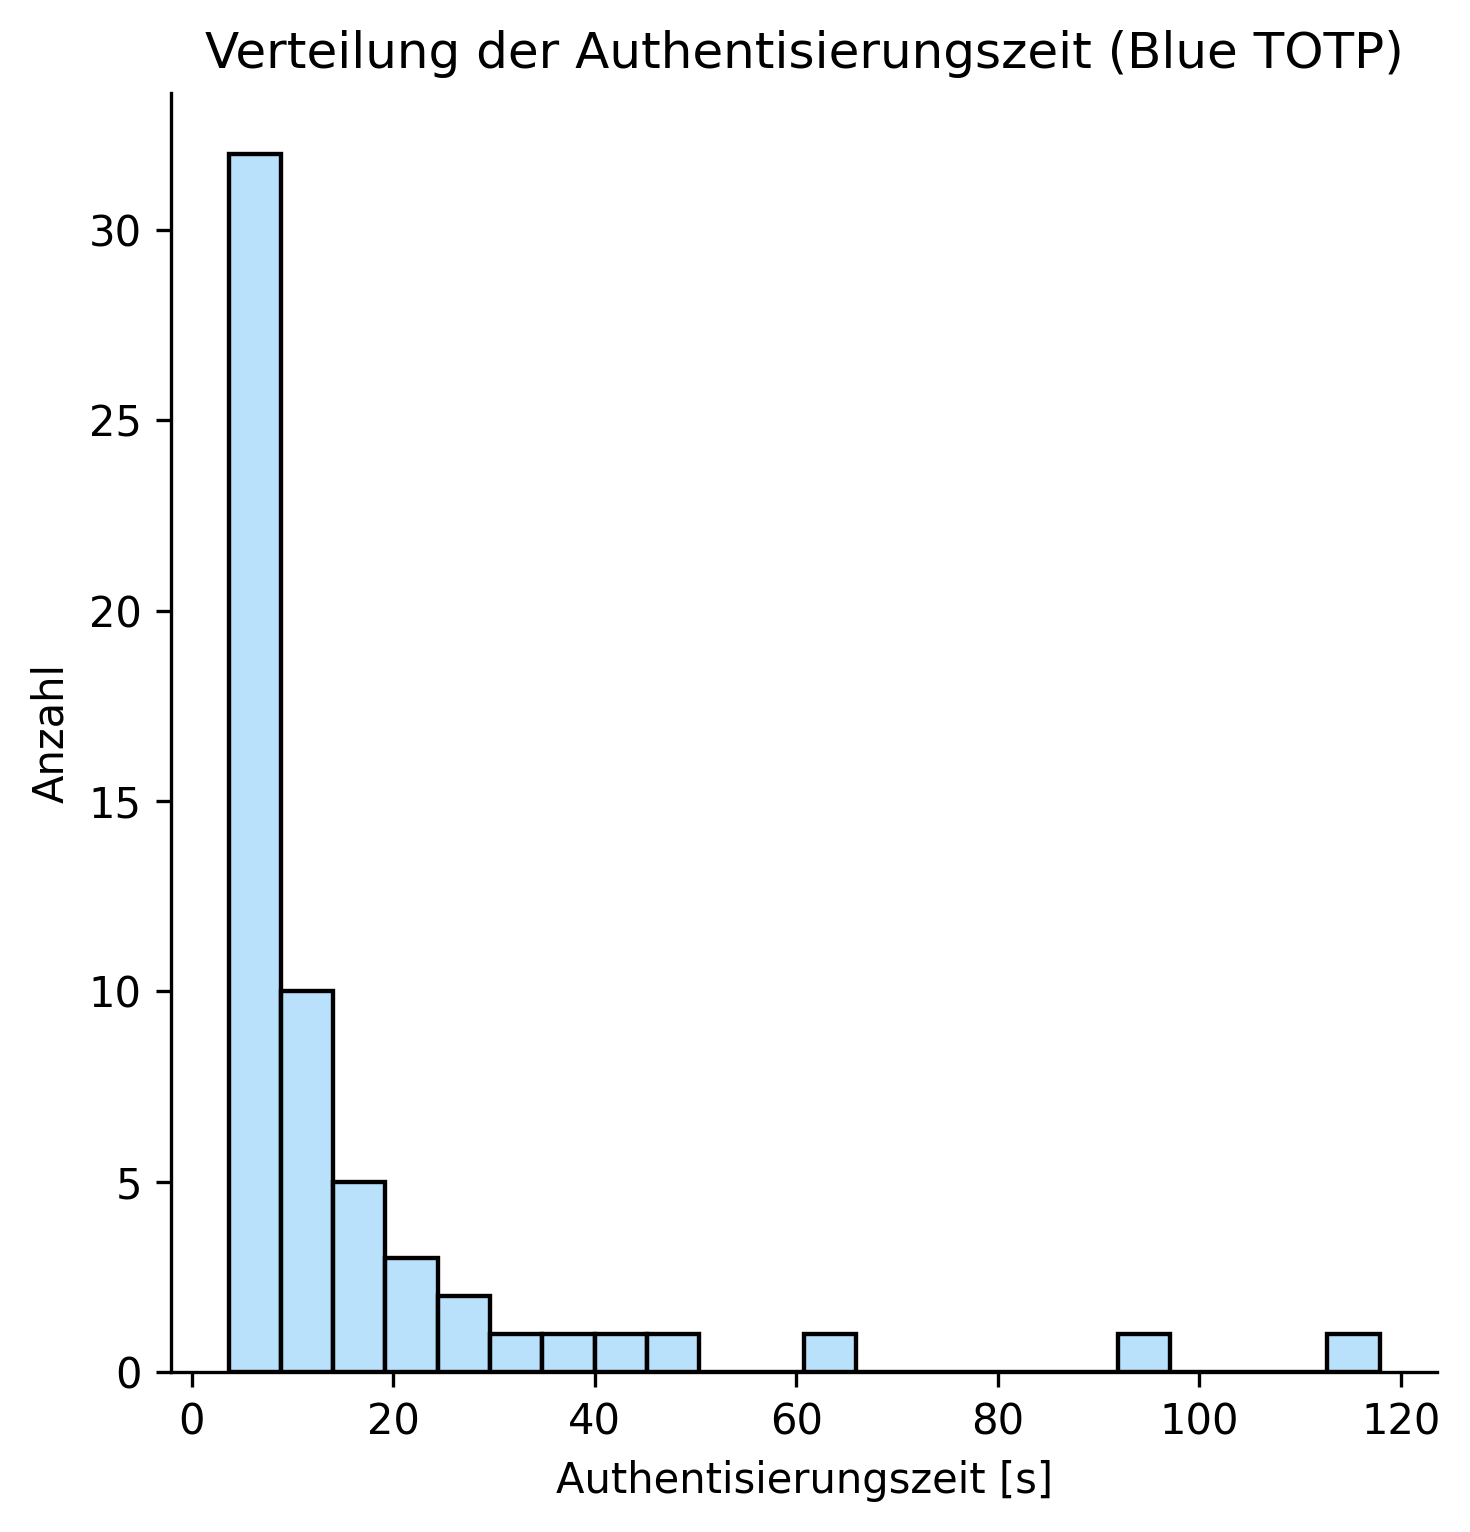
\includegraphics[width=1\linewidth]{data_processing/timings/results/distribution_of_data.png}
        \caption[Verteilung der Authentisierungszeiten (Blue TOTP)]{Verteilung der Authentisierungszeiten (Blue TOTP)}
        \label{fig: studie ergebnisse auth time dist}
    \end{minipage}
    \hfill
    \begin{minipage}[t]{.48\textwidth}
        \centering
        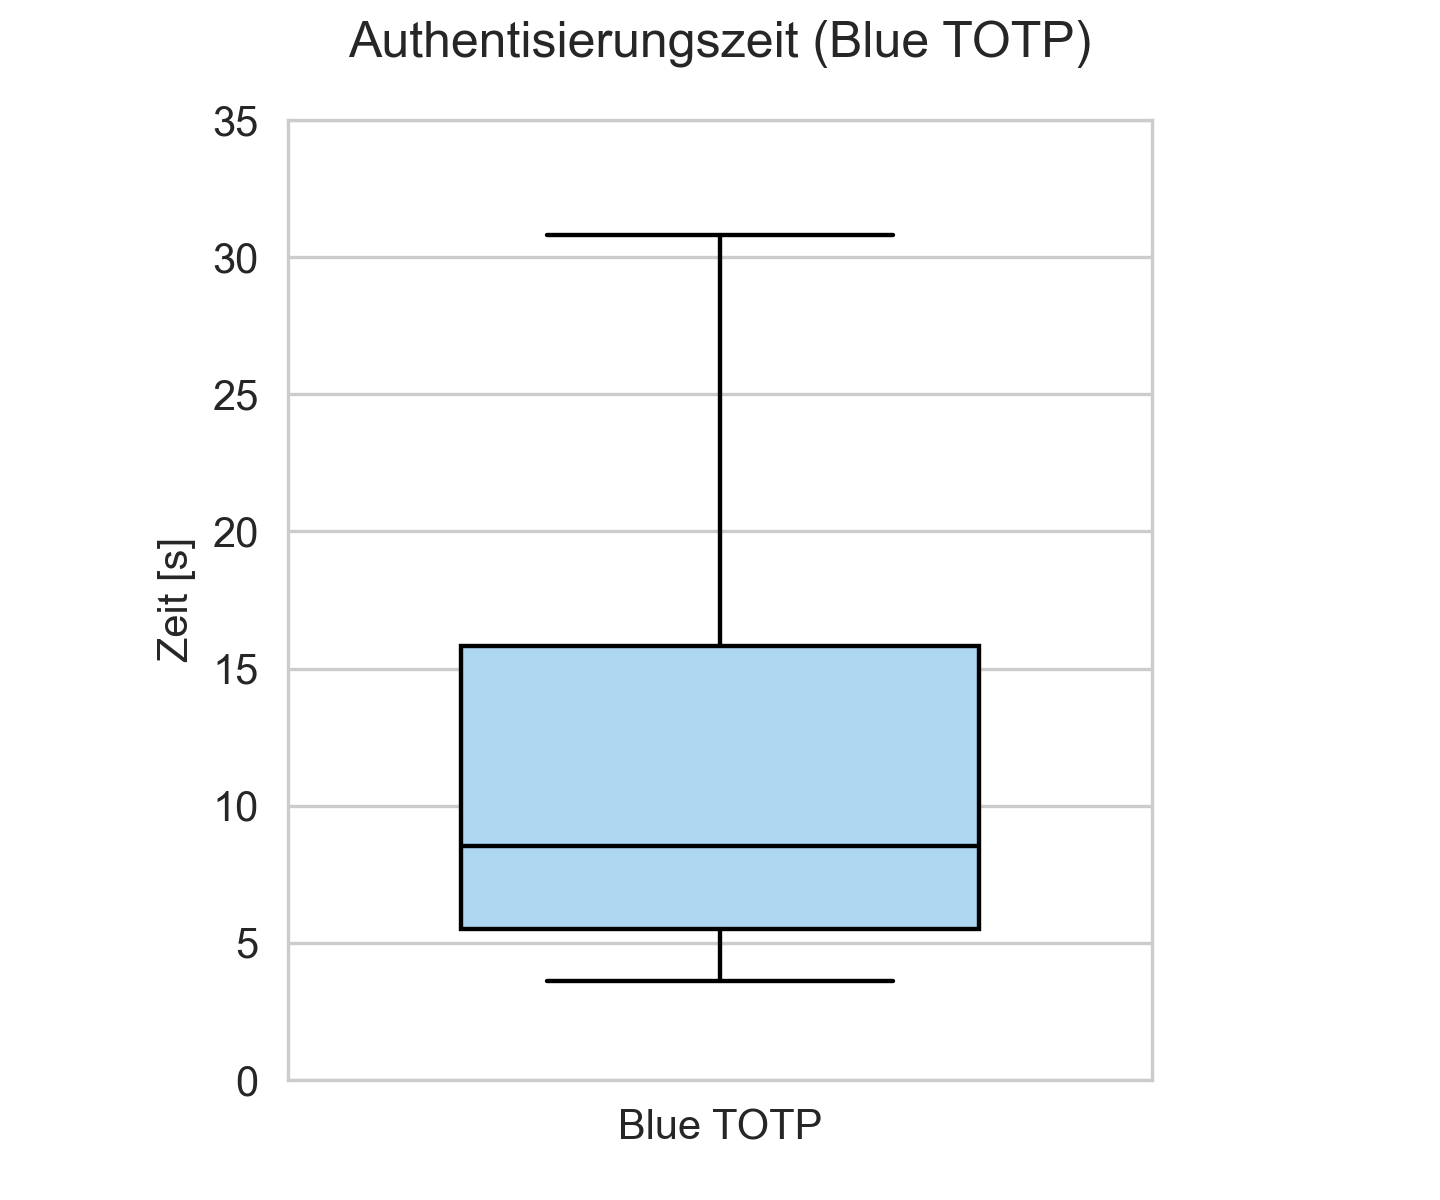
\includegraphics[width=1.2\linewidth]{data_processing/timings/results/totp_timings_boxplot.png}
        \caption[Authentisierungszeit von Blue TOTP]{Authentisierungszeit von Blue TOTP}
        \label{fig: studie ergebnisse auth time boxplot}
    \end{minipage}
\end{figure}
Über 30 der 59 Werte liegen unter $10~s$. Die kürzeste Messung beträgt $3{,}6~s$. Es gibt einige Ausreißer wie die drei über 
$60~s$. Es ist unklar, wieso die Probanden bei diesen Messungen übermäßig Zeit 
benötigten. Alle Messungen bilden einen Median von $8{,}5~s$ und einen Mittelwert von 
$15{,}9~s$. Bereinigt man die Daten nach dem Verfahren des $1{,}5$-fachen 
Interquartilsabstands (Entfernen aller Werte $> 31{,}3~s$), erhält man einen 
Mittelwert von $10,1~s$ (siehe Anhang \ref{anh: studie ergebnisse auth} Tab. \ref{tab: 
studie ergebnisse auth time}).
\\\\
Die Authentisierungszeiten pro Tag der Nutzungsphase sind in Abb. \ref{fig: studie 
ergebnisse auth time days} dargestellt. Das Diagramm zeigt nur den Wertebereich bis 
$40~s$, um die dichten Datenpunkte besser zu unterscheiden.
\begin{figure}
    \centering
    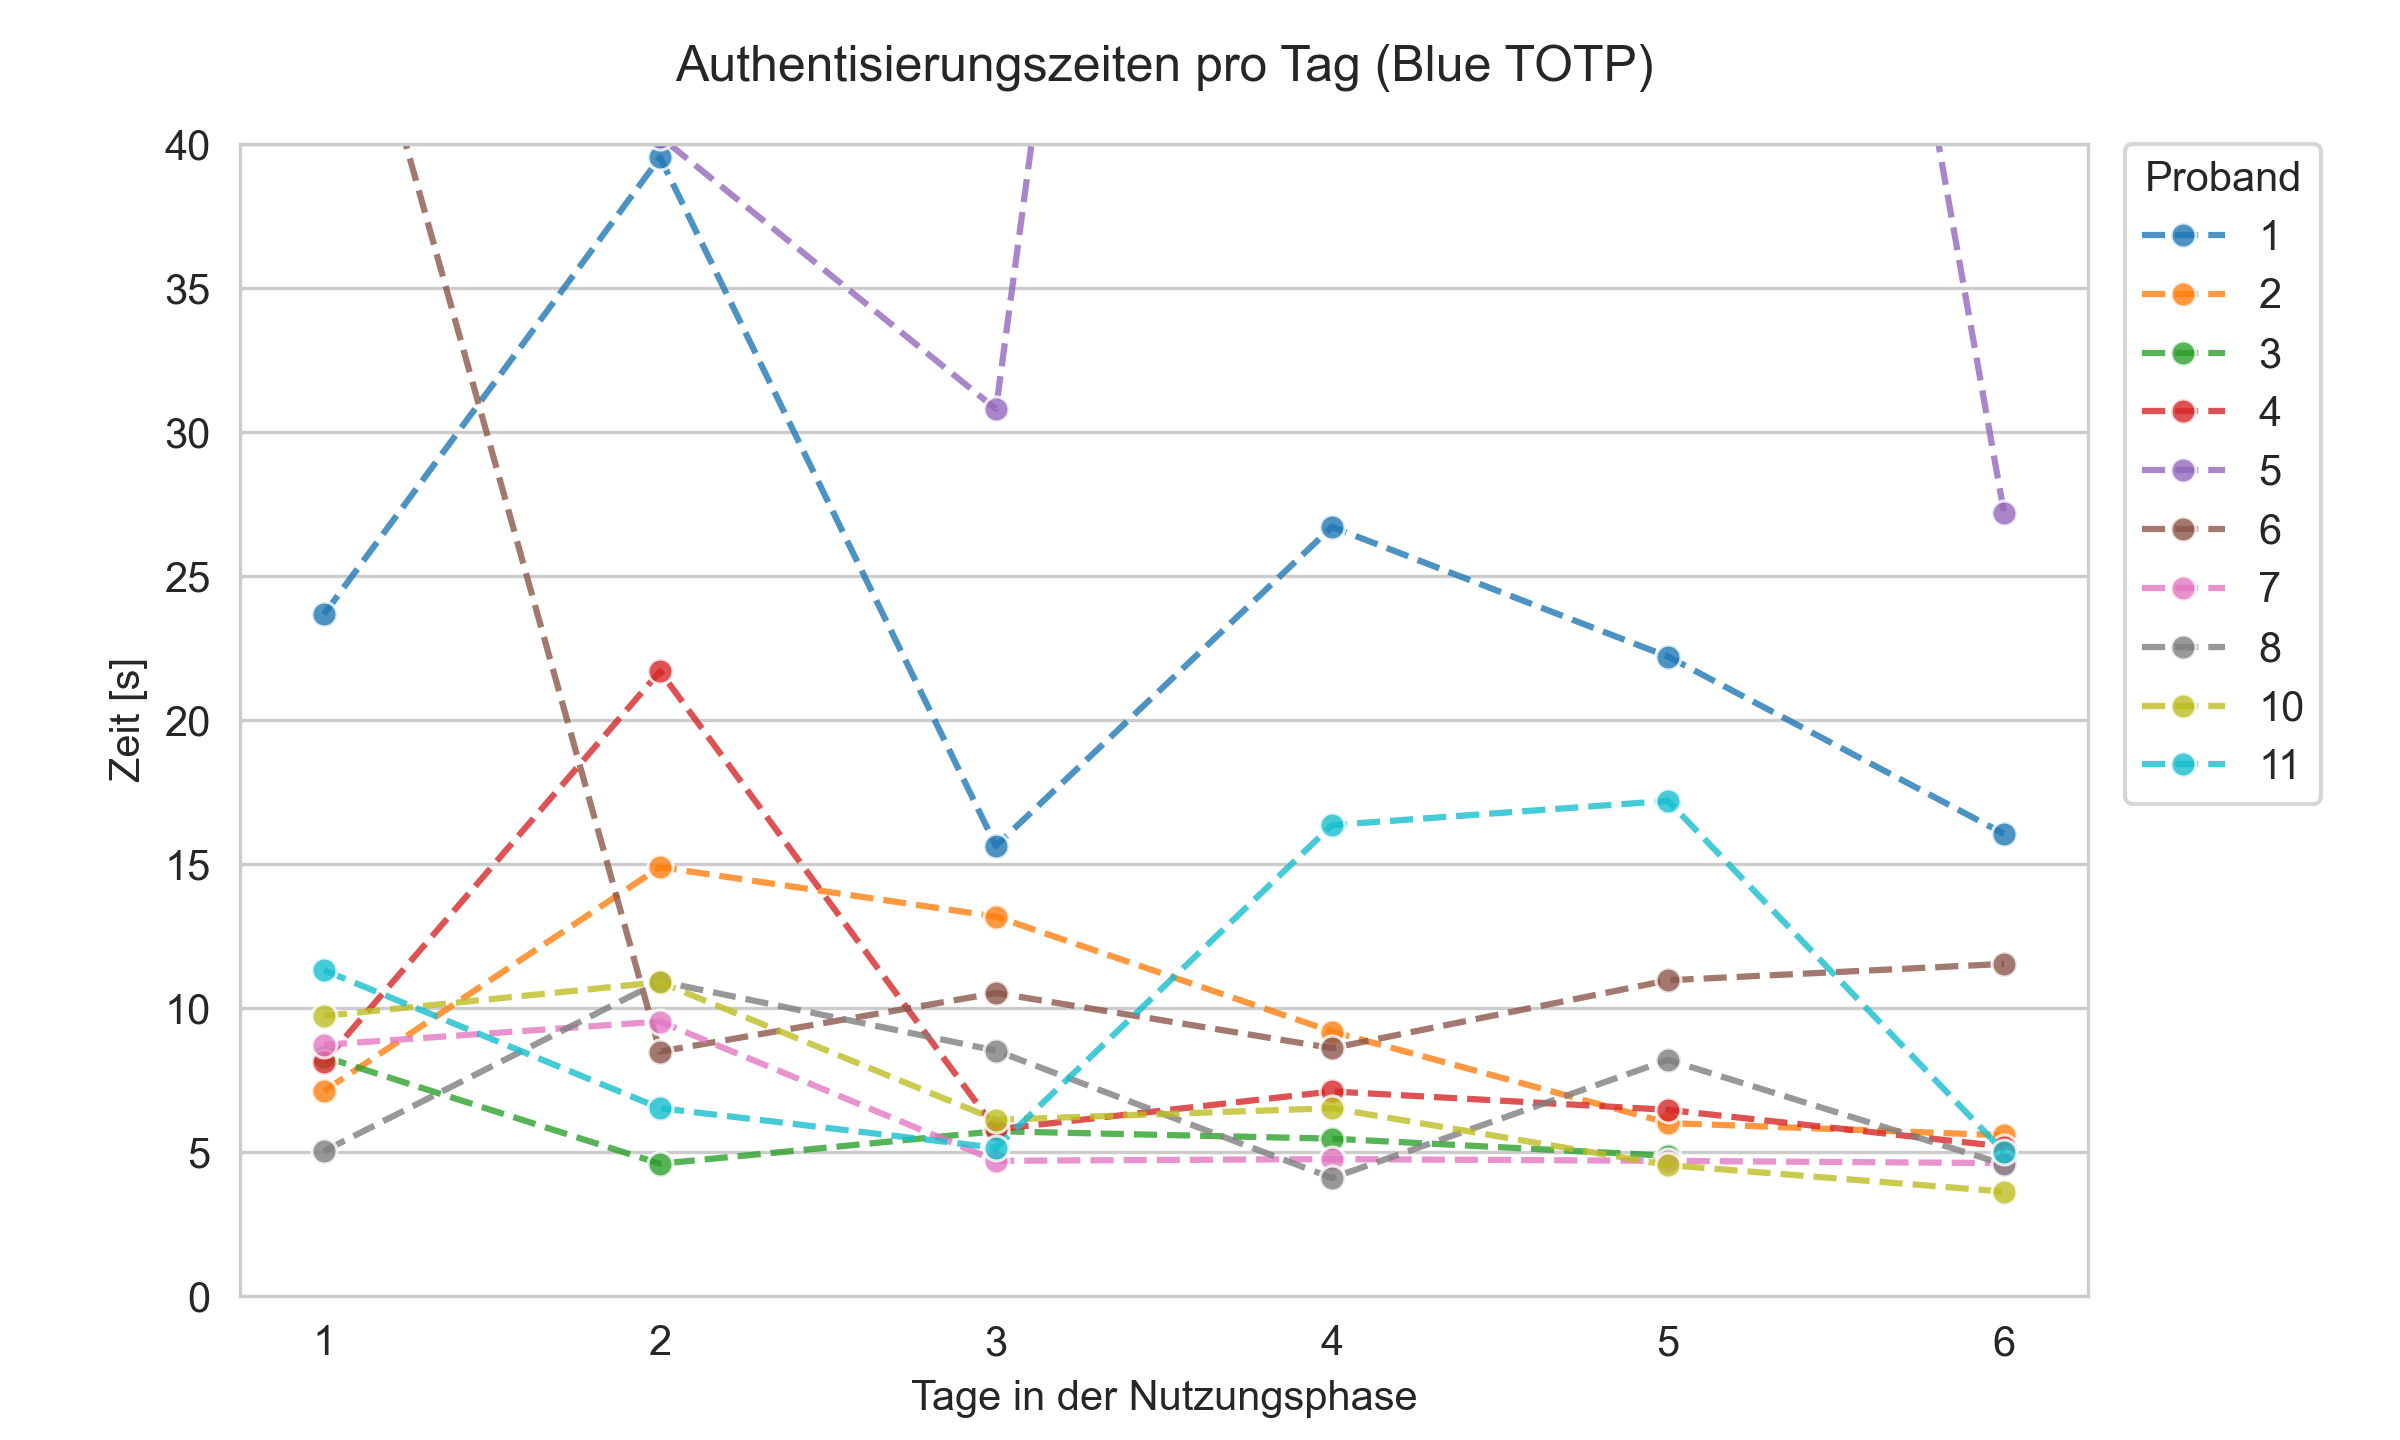
\includegraphics[width=0.85\linewidth]{data_processing/timings/results/totp_timings_lineplot.png}
    \caption[Authentisierungszeiten pro Tag in der Nutzungsphase (Blue TOTP)]{Authentisierungszeiten pro Tag in der Nutzungsphase (Blue TOTP)}
    \label{fig: studie ergebnisse auth time days}
\end{figure}
Die Verläufe der einzelnen Linien lässt im Gesamtbild keine klare Tendenz erkennen, 
ob die Probanden über die Dauer der Nutzungsphase die Authentisierung immer schneller 
durchführten. Lässt man die Probanden 1,5 und 6 außen vor, erkennt man, dass die 
verbleibenden 7 Probanden bis auf einzelne Ausnahmen immer weniger als $15~s$ 
benötigt haben. Auch ist erkennbar, dass diese 7 Probanden am letzten Tag nur ca. 
$5~s$ benötigten und im Vergleich zum ersten Tag schneller waren. Betrachtet man die 
Medianwerte aller Messungen pro Tag in der Nutzerstudie, wie in Tab. \ref{tab: studie 
ergebnisse auth time median days} dargestellt, dann lässt sich dahingehend auch ein 
Trend erkennen.
\begin{table}
    \centering
    \begin{center}
    \begin{tabular}{| l | c | c | c | c | c | c |}
        \hline
        \textbf{Tag} & $1$ & $2$ & $3$ & $4$ & $5$ & $6$ \\
        \hline
        \textbf{Median} & $9{,}2~s$ & $10{,}9~s$ & $7{,}3~s$ & $7{,}9~s$ & $7{,}3~s$ & $5{,}2~s$ \\
        \hline
    \end{tabular}
    \end{center}
    \caption[Median der Authentisierungszeit pro Tag in der Nutzungsphase]{Median der Authentisierungszeit pro Tag in der Nutzungsphase}
    \label{tab: studie ergebnisse auth time median days}
\end{table}
Die Analyse mithilfe der Repeated Measures Correlation zwischen den Tagen der 
Nutzungsphase und den Authentisierungszeiten pro Proband ergab einen 
Korrelationskoeffizienten von $r = -0{,}1634$ und keine statistische Signifikanz, da 
$p > 0{,}05$ (siehe Anhang \ref{anh: studie ergebnisse auth} Tab. \ref{tab: studie 
ergebnisse auth time rmcorr}). Dennoch ist die negative Richtung der Korrelation 
zwischen Tag der Nutzungsphase und Authentisierungszeit deutlich.
\\\\
Bei dem Versuch, die tägliche Aufgabe im Webservice zu lösen, kam es bei 23 der 
insgesamt 59 Sitzungen vor, dass die Probanden Benutzername und Passwort mindestens 
einmal erneut eingeben mussten, wahrscheinlich weil sie die App und Extension 
nicht vor der Eingabe von Benutzername und Passwort miteinander verbunden hatten. In diesem Fall wurde das TOTP nicht automatisch von der 
App an die Extension übertragen. Insgesamt gab es 36 fehlgeschlagene 
Loginversuche.

        \subsubsection{User Experience Questionnaire}
            \label{sec: ergebnisse studie auth ueq}
            Die Probanden haben den UEQ bzgl. der Authentisierung einmal für das traditionelle 
TOTP-Verfahren und einmal für Blue TOTP ausgefüllt. Es sollte nur die Authentisierung 
mit dem jeweiligen Verfahren beurteilt werden, also auch die Handhabung der TOTP-App. 
Das Design von Website bei der Anmeldung sollte kein Bestandteil der Beurteilung sein.
\\\\
In Abb. \ref{fig: studie ergebnisse auth ueq bt trad single} sind die Mittelwerte jedes Gegensatzpaares dargestellt.
\begin{figure}
    \centering
    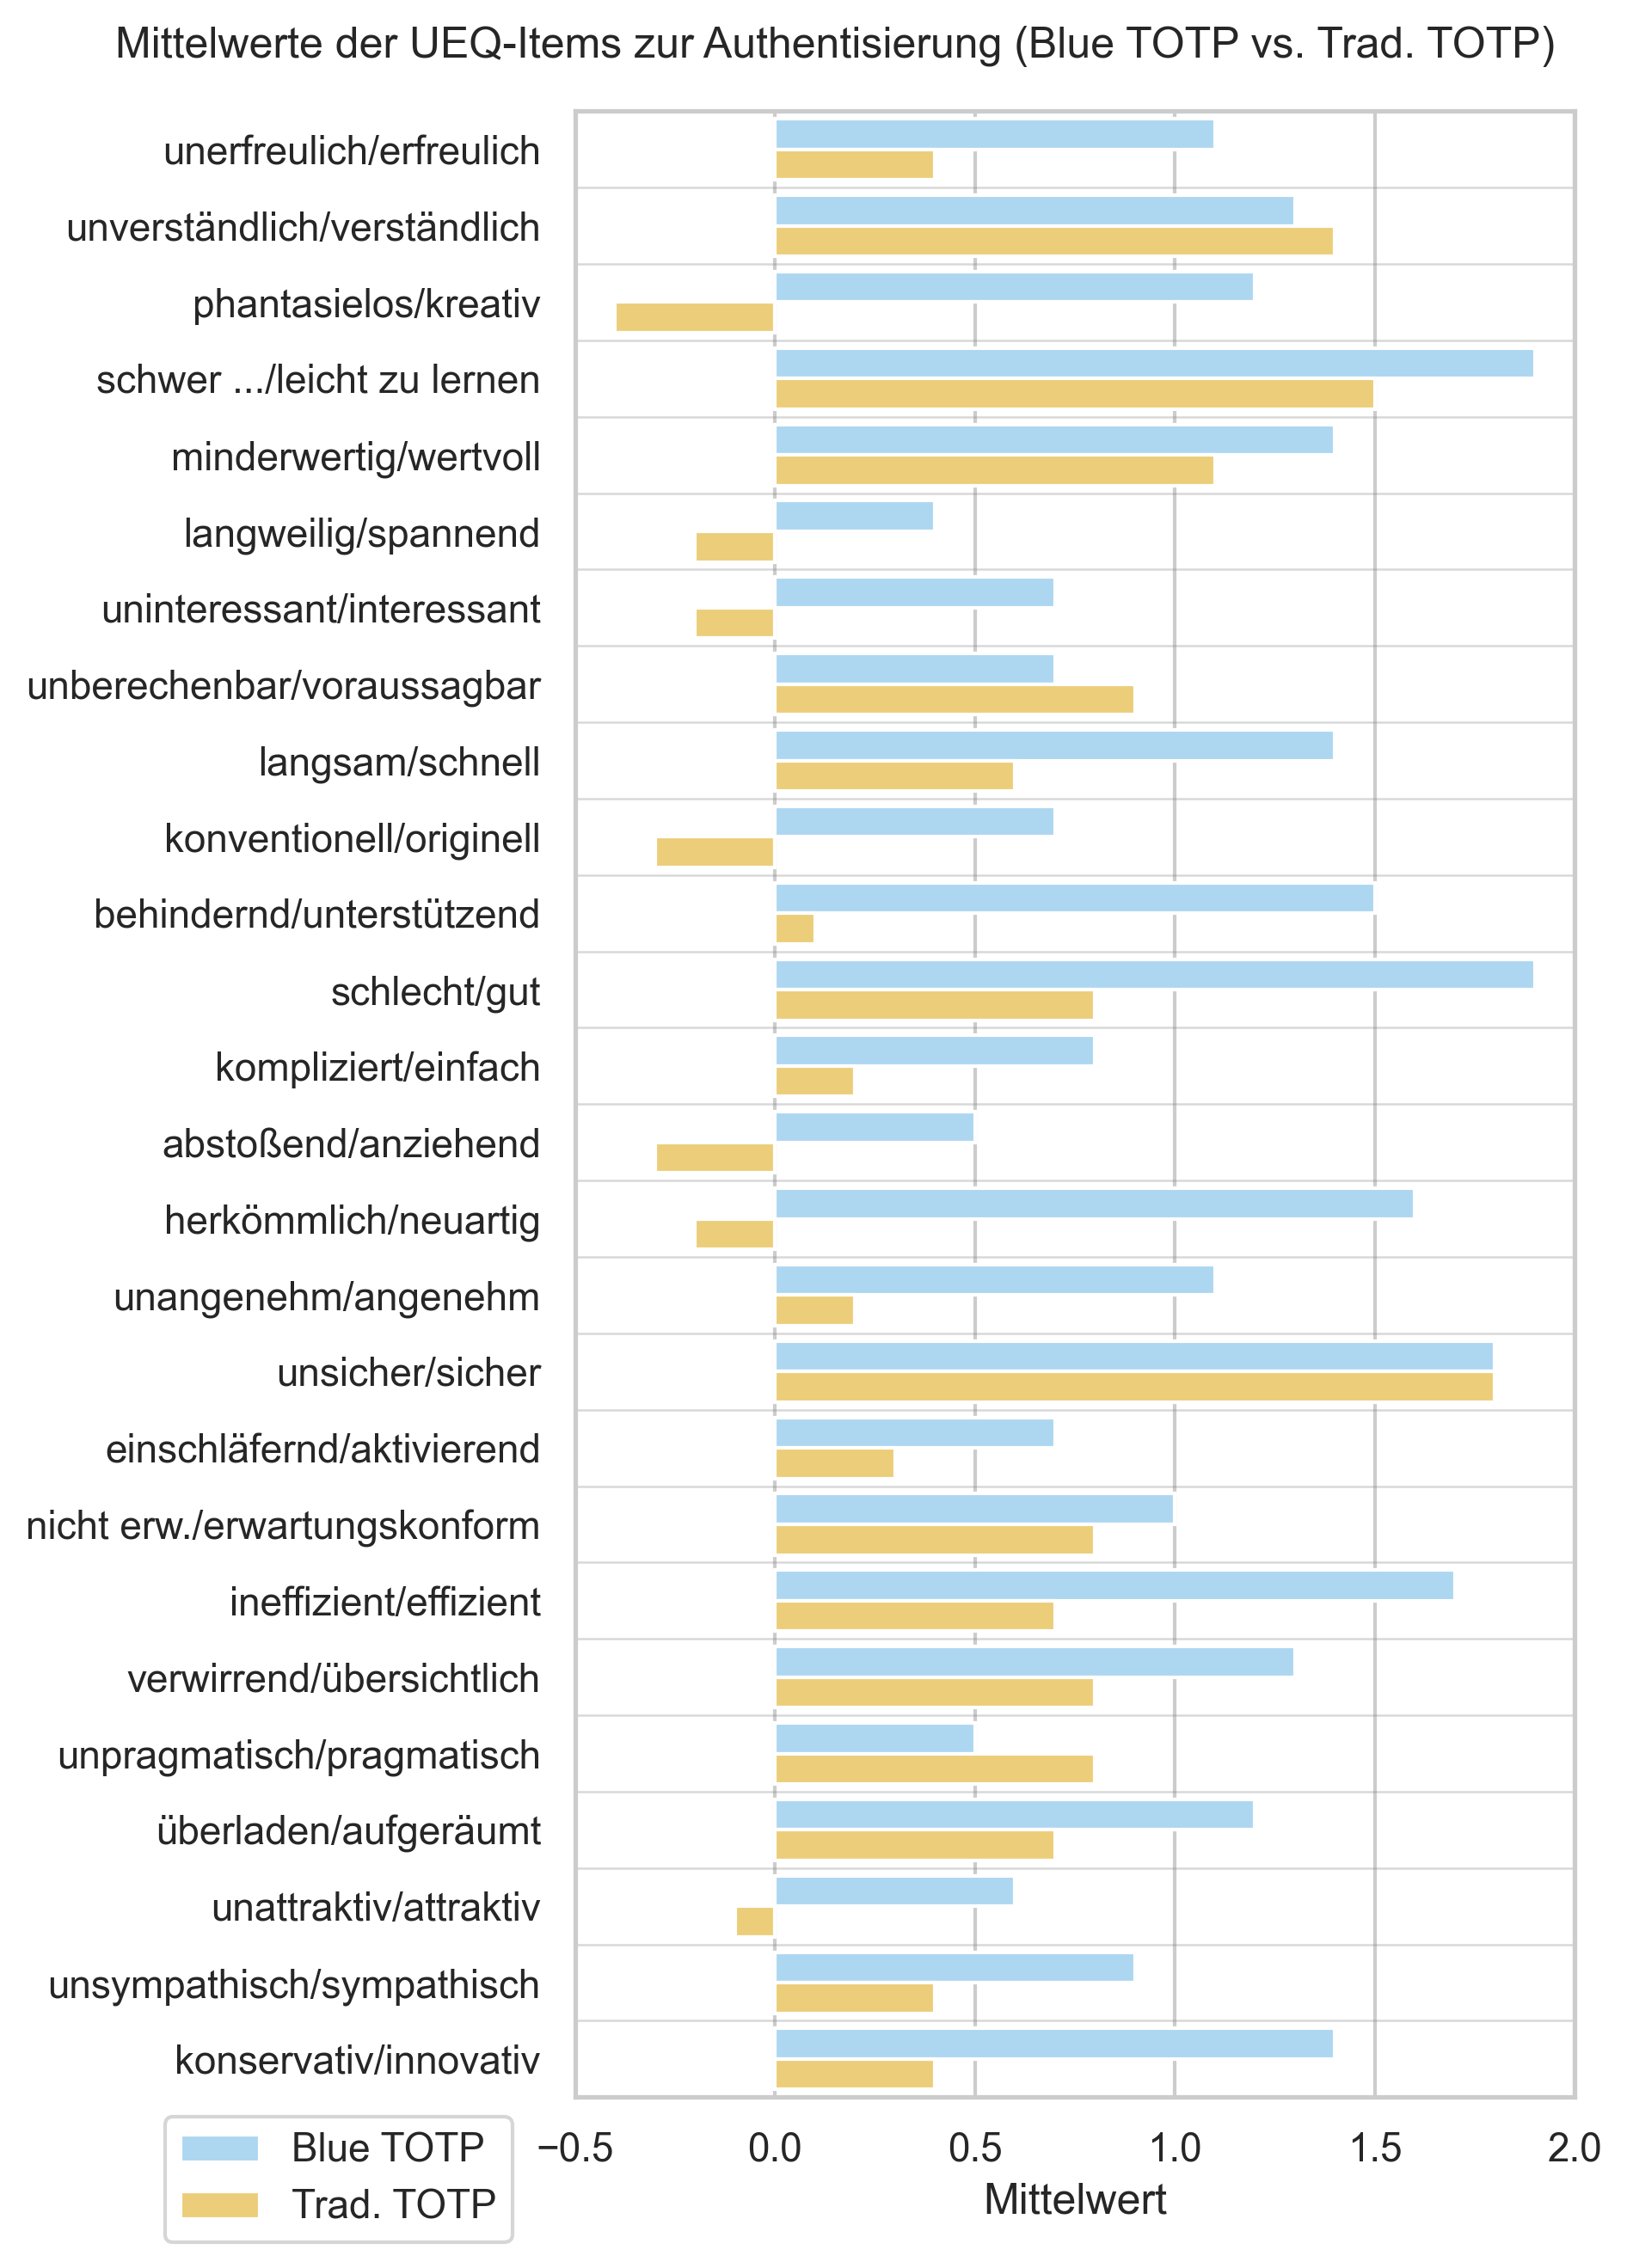
\includegraphics[width=0.65\linewidth]{data_processing/questionaires/results/from_ueq_excel/ueq_single_means_bt_trad.png}
    \caption[Mittelwert pro Gegensatzpaar des UEQ (Blue TOTP vs. trad. TOTP)]{Mittelwert pro Gegensatzpaar des UEQ (Blue TOTP vs. trad. TOTP)}
    \label{fig: studie ergebnisse auth ueq bt trad single}
\end{figure}
Es ist auffällig, dass viele Mittelwerte der hedonischen Gegensatzpaare (zugehörig zu 
Stimulation und Originalität) gegensätzlich sind.
Beispiele sind \glqq phantasielos/kreativ\grqq{}, \glqq langweilig/spannend\grqq{} 
und \glqq herkömmlich/neuartig\grqq{}. 
Bei diesen hedonischen Paaren liegt der Mittelwert für das traditionelle 
TOTP-Verfahren überwiegend im negativen Bereich zwischen $0$ und $-0{,}5$. Generell 
erkennt man, dass Blue TOTP überwiegend einen höheren Mittelwert erreicht als das 
traditionelle Verfahren. Einige dieser Gegensatzpaare sind \glqq unerfreulich/
erfreulich\grqq{} mit $\bar{x}_{Blue} = 1{,}1$ zu $\bar{x}_{Trad} = 0{,}4$ oder \glqq 
langsame/schnell\grqq{} mit $\bar{x}_{Blue} = 1{,}4$ zu $\bar{x}_{Trad} = 0{,}6$. 
Auch die für Blue TOTP positive Differenz bei \glqq behindernd/unterstützend\grqq{} 
($1{,}4$) sowie \glqq unangenehmen/angenehm\grqq{} ($0{,}9$) ist bemerkenswert. 
Nicht sonderlich unerwartet ist der Gleichstand bei \glqq unsicher/sicher\grqq{}. Nur 
bei den Kriterien, wie pragmatisch und verständlich es ist, steht Blue TOTP dem 
traditionellen Verfahren nach mit einer geringen Differenzen von $\le 0{,}3$.
\\\\
Der Vergleich beider Systeme bzgl. der UEQ-Skalen ist in Abb. \ref{fig: studie 
ergebnisse auth ueq overview} dargestellt.
\begin{figure}
    \centering
    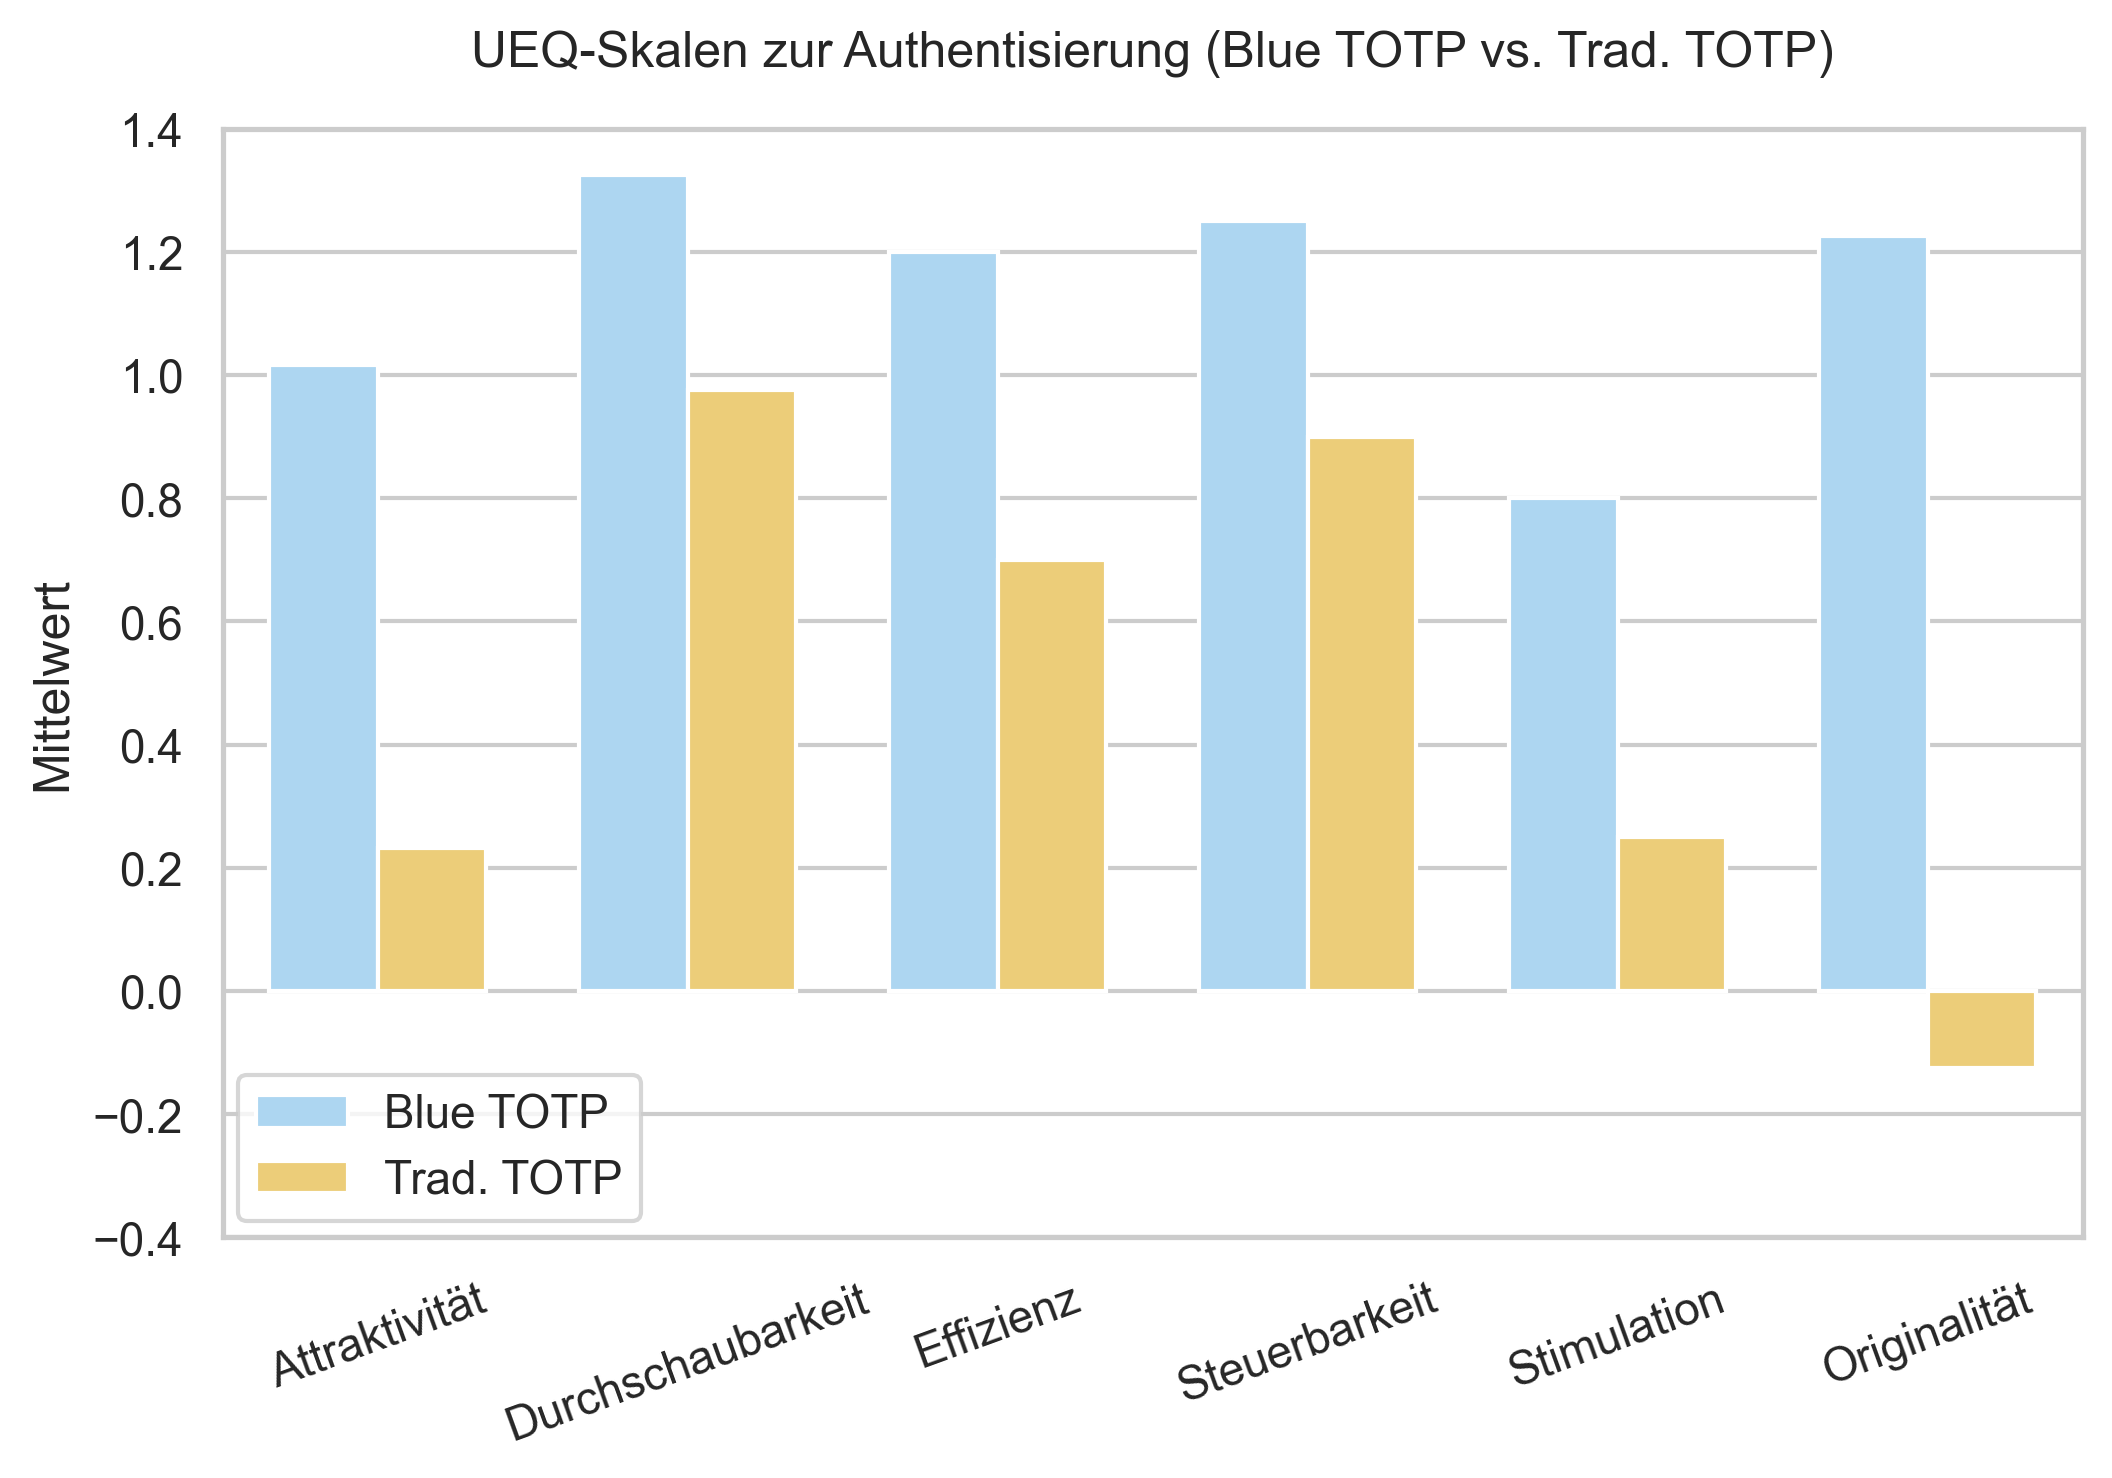
\includegraphics[width=0.75\linewidth]{data_processing/questionaires/results/from_ueq_excel/ueq_overview_bt_trad.png}
    \caption[Vergleich der UEQ-Skalen zur Authentisierung (Blue TOTP vs. trad. TOTP)]{Vergleich der UEQ-Skalen zur Authentisierung (Blue TOTP vs. trad. TOTP)}
    \label{fig: studie ergebnisse auth ueq overview}
\end{figure}
Statistische Signifikanz für $\alpha = 0{,}05$ zwischen Blue TOTP und dem trad. TOTP wurde bei den Skalen Attraktivität ($p = 0{,}0183$) und Originalität ($p = 0{,}004$) erreicht (t-Test). Dazu wurde ein Zweistichproben-t-Test verwendet. Wie bereits bei den einzelnen Gegensatzpaaren beobachtet, übertrifft Blue TOTP das 
traditionelle Verfahren im Mittelwert jeder Skala. Die höchste Differenz bildet sich 
in der Originalität mit $1{,}1$. Auch die Stimulation ist um einen Wert von fast $0{,}
6$ höher. Allerdings sollte man beachten, dass laut \textcite{Schrepp} der positive 
Bewertungsbereich erst bei $0{,}8$ (aufsteigend) beginnt. Demnach ist Stimulation bei 
Blue TOTP nichts außergewöhnliches. Auch sollte man sich des potentiellen Minimums 
von $-3$ bzw. des Maximums von $3$ bewusst sein. Die anderen Skalen hinsichtlich der 
Forschungsfragen sind von mehr Bedeutung. Damit ist vor allem die 
Attraktivität und die Effizienz gemeint. Bei der Attraktivität ist zu Gunsten von 
Blue TOTP eine Verfünffachung von ca. $0{,}2$ auf $1{,}0$ zu verzeichnen. Auch bei 
der Effizienz ist ein positiver Effekt zu verzeichnen. Im Vergleich zum 
traditionellen Verfahren erstreckt sich jede Skala von Blue TOTP (mit Ausnahme der 
Stimulation) bis deutlich über die Grenze zwischen dem neutralen und positiven 
Bewertungsbereich.
        
        \subsubsection{System Usability Scale}
            \label{sec: ergebnisse studie auth sus}
            Der SUS-Fragebogen wurde den Probanden unter den gleichen Anforderungen vorgelegt 
(Bezug nur auf das Verfahren bei der Authentisierung und die TOTP-App).
In Abb. \ref{fig: studie ergebnisse auth sus boxplot} sowie Tab. \ref{tab: studie 
ergebnisse auth sus boxplot} werden Blue TOTP und das traditionelle TOTP-Verfahren 
gegenübergestellt.
\begin{figure}
    \centering
    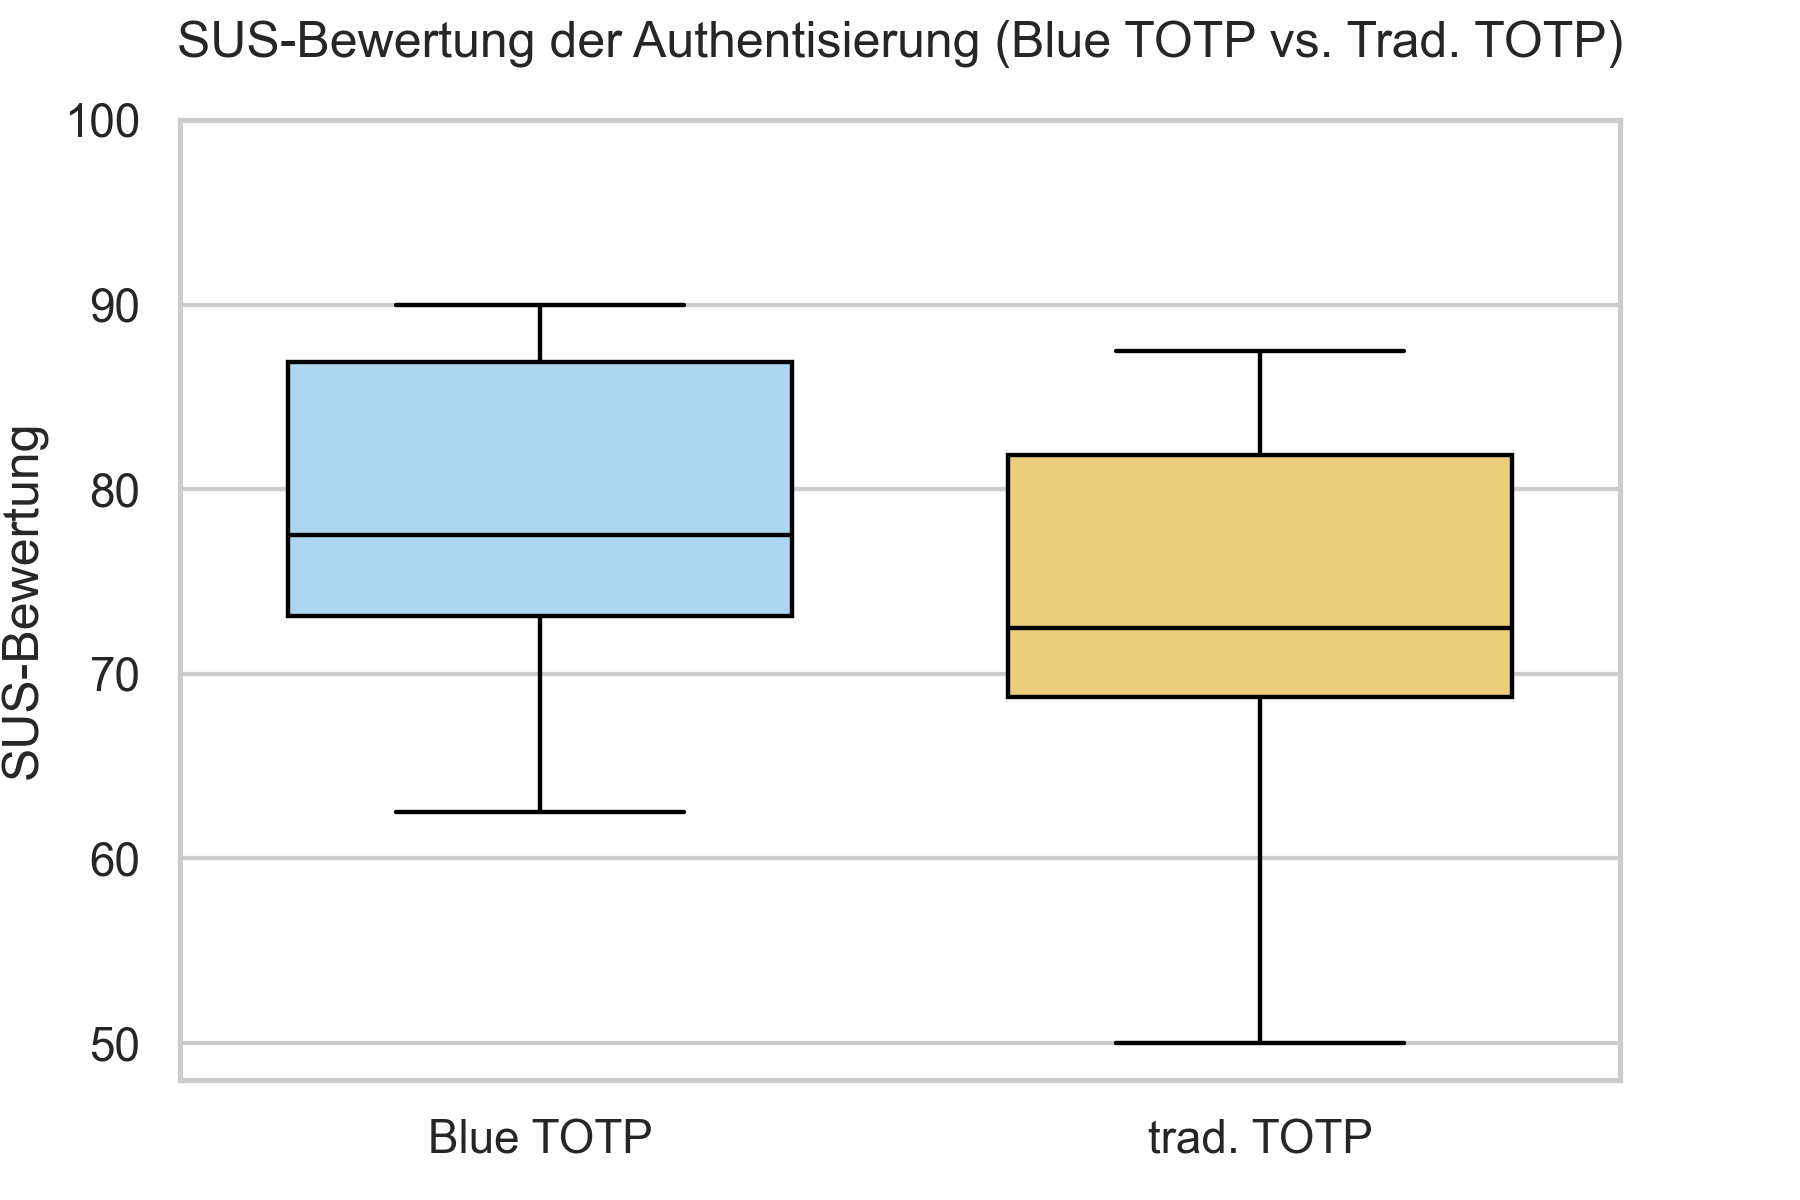
\includegraphics[width=0.6\linewidth]{data_processing/questionaires/results/usage_sus_boxplot.png}
    \caption[SUS-Bewertung der Authentisierung (Blue TOTP vs. trad. TOTP)]{SUS-Bewertung der Authentisierung (Blue TOTP vs. trad. TOTP)}
    \label{fig: studie ergebnisse auth sus boxplot}
\end{figure}
\begin{table}
    \begin{center}
    \begin{tabular}{| l | c | c | c | c |}
        \hline
        \textbf{Verfahren} & \textbf{Q1} & \textbf{Median} & \textbf{Mittelwert} & \textbf{Q3}  \\
        \hline
        Blue TOTP & 73 & 78 & 79 & 87 \\
        \hline
        Trad. TOTP & 69 & 73 & 73 & 82 \\ 
        \hline
    \end{tabular}
    \end{center}
    \caption[SUS-Bewertung der Authentisierung (Blue TOTP vs. Trad. TOTP)]{SUS-Bewertung der Authentisierung (Blue TOTP vs. Trad. TOTP)}
    \label{tab: studie ergebnisse auth sus boxplot}
\end{table}
Das Boxplot deutet darauf hin, dass die Verteilung der SUS-Bewertungen beider 
Verfahren im Interquartilbereich sich ähneln und nur auf der Y-Achse verschoben sind. 
Es ist deutlich erkennbar, dass das traditionelle in allen Werten Blue TOTP 
nachsteht. Die Normalverteilung der Differenzen der SUS-Berwertungen pro Proband wurde mit dem Shapiro-Wilk-Test bestätigt ($p=0{,}4439$) und daher ein Paired t-Test für die SUS-Bewertungen durchgeführt. Allerdings konnte keine statistische Signifikanz zwischen den beiden SUS-Bewertungen festgestellt werden ($p=0{,}2366$, $\alpha = 0{,}05$). Blue TOTP erzielt einen Median von 78 Punkten und das traditionelle 
Verfahren nur 73 Punkte. Dieser Abstand von ca. 5 Punkten lässt sich auch bei den 
anderen Größen 1. Quartil, Mittelwert und 3. Quartil beobachten, die zwischen 4 bis 6 
Punkten auseinander liegen (vergl. Tab. \ref{tab: studie ergebnisse auth sus 
boxplot}). Folgt man den Erkenntnissen von \textcite{Sauro}, so liegt dieser Bereich 
im annähernd linearen Verlauf der S-Kurve, die den prozentualen Wert einer 
SUS-Punktzahl wiedergibt. Demnach wäre der eben beschriebene  Unterschied von ca. 5 
Punkten linear zum prozentualen Wert (nicht im Verhältnis 1:1).
\\\\
Auch diesmal haben die Probanden am Ende des Fragebogens die empfundene 
Nutzerfreundlichkeit angegeben. Die SUS-Bewertungen und entsprechenden 
SUS-Punktzahlen zu der empfundenen Nutzerfreundlichkeit sind in Abb. \ref{fig: studie 
ergebnisse auth sus vs 11} dargestellt.
\begin{figure}
    \centering
    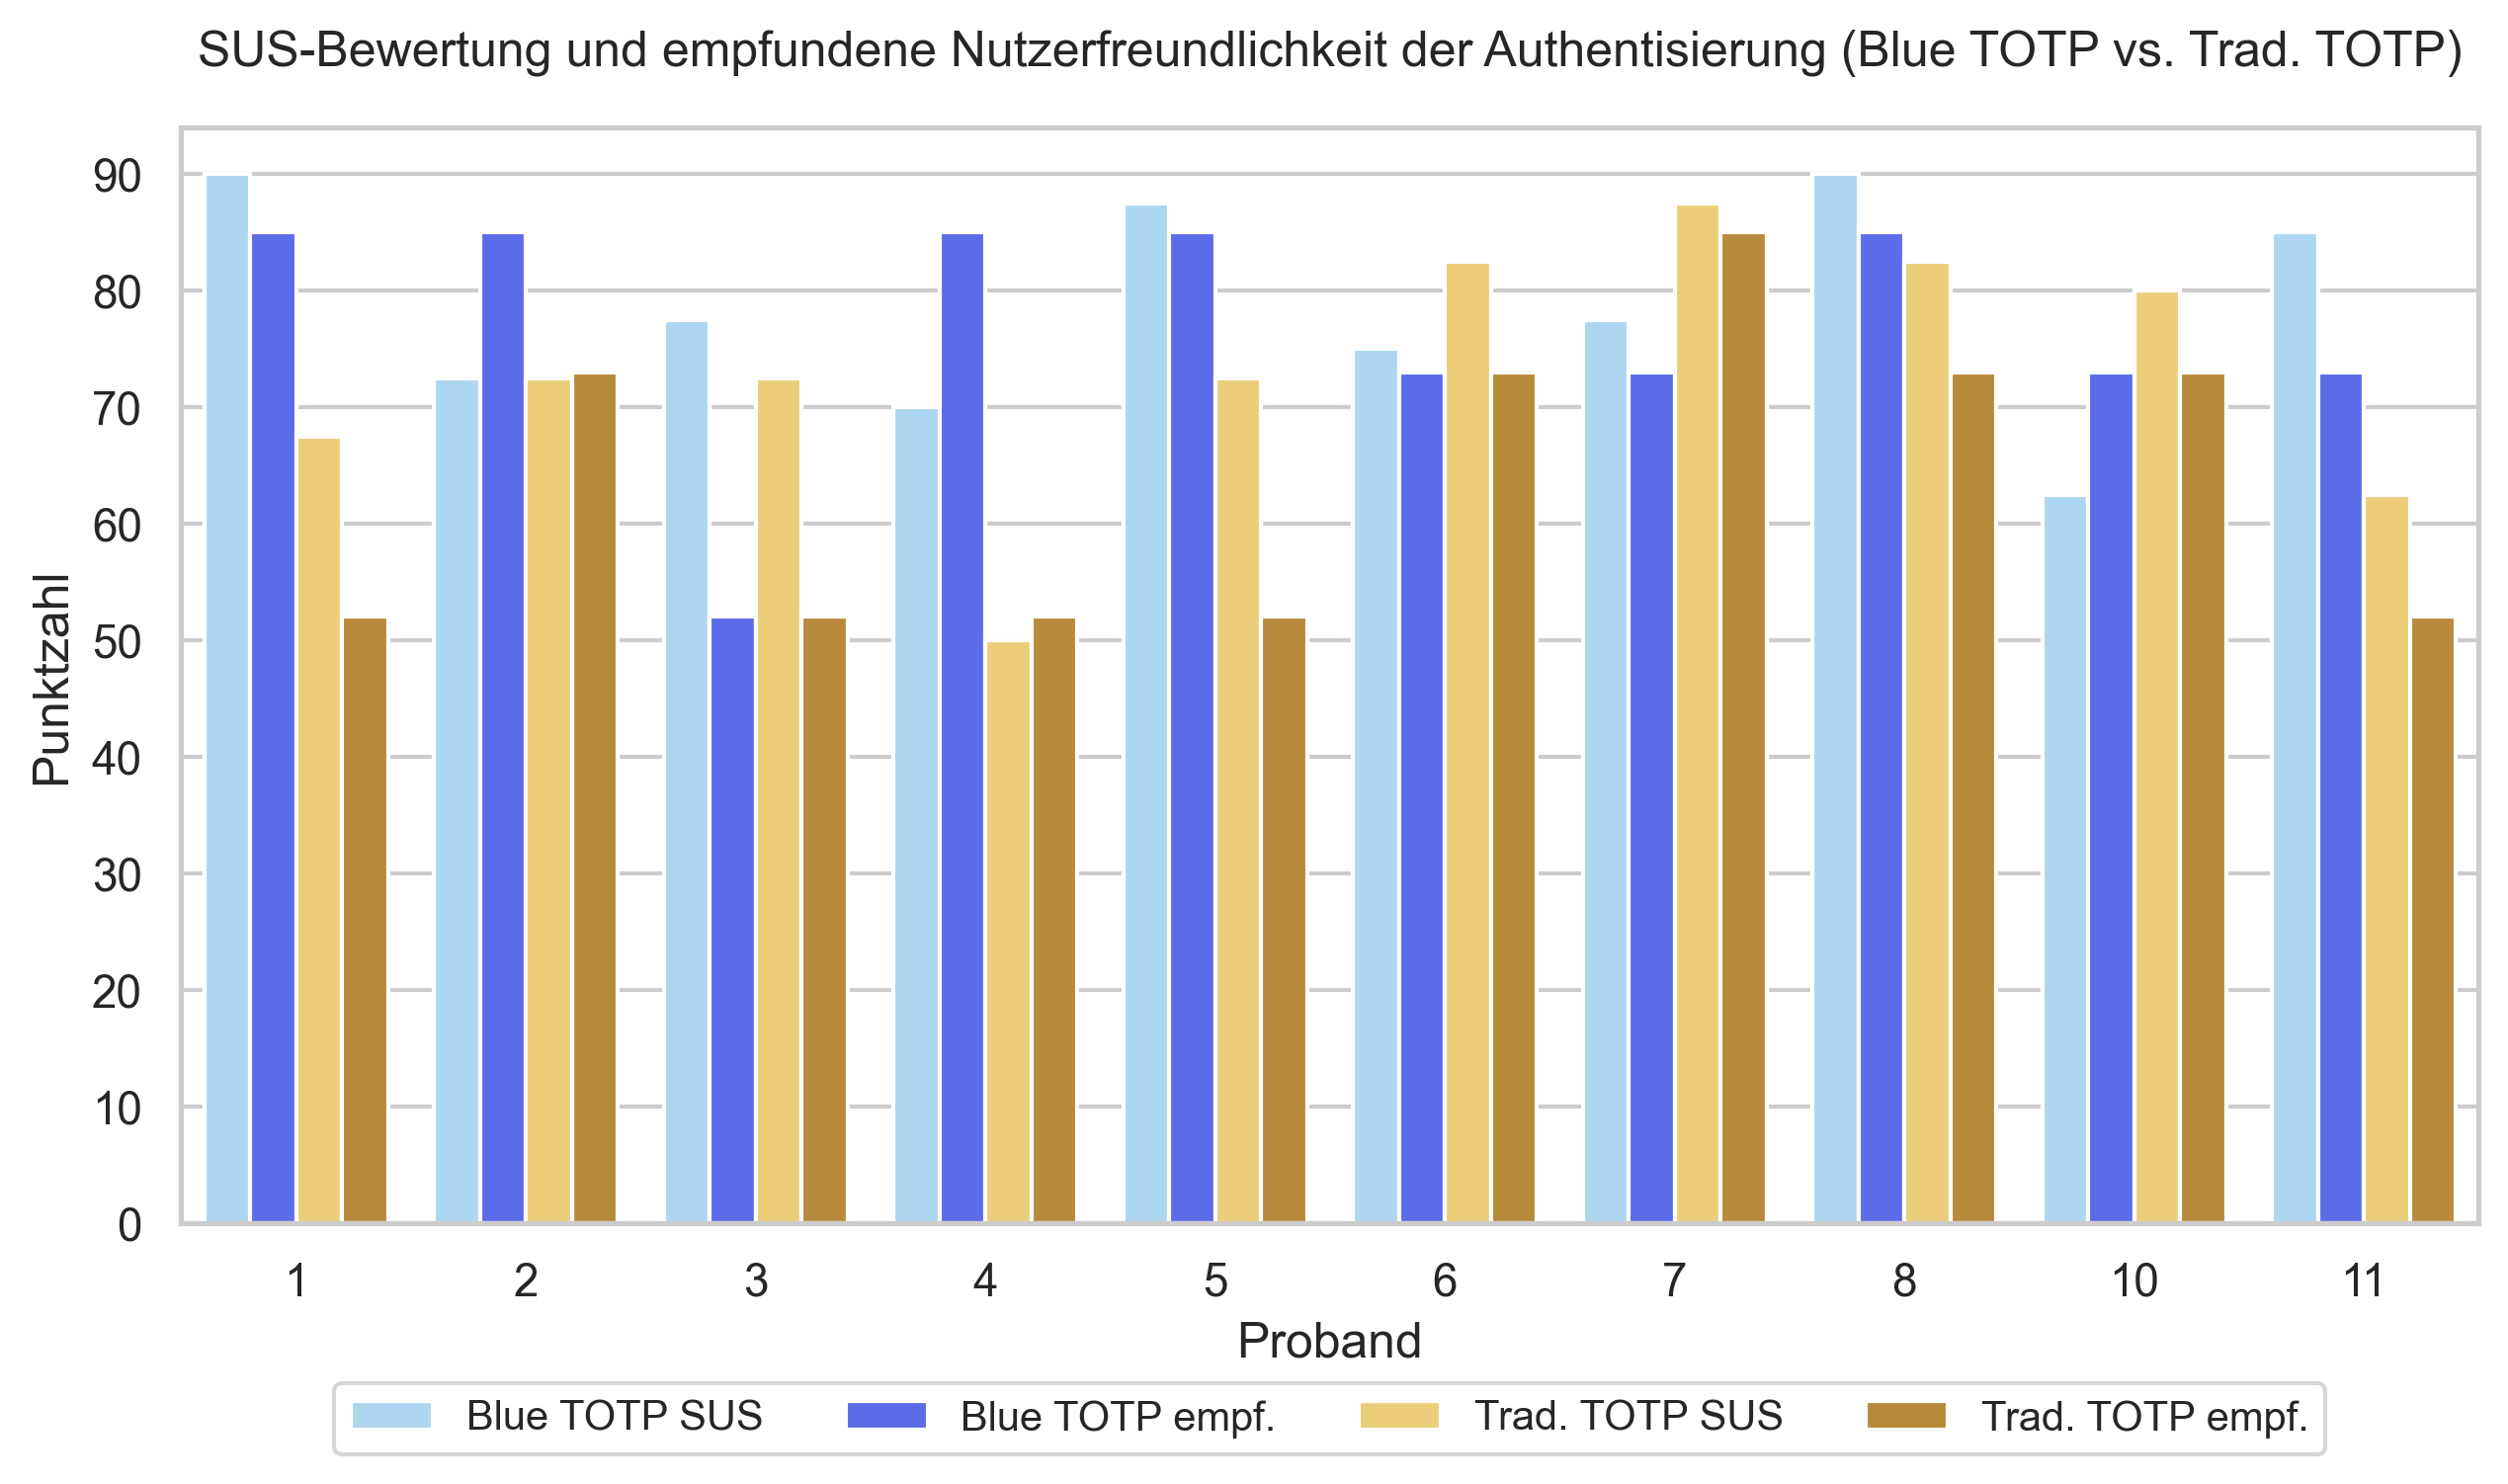
\includegraphics[width=0.8\linewidth]{data_processing/questionaires/results/usage_sus_vs_sus11.png}
    \caption[SUS-Bewertung und empfundene Nutzerfreundlichkeit (Authentisierung)]{SUS-Bewertung und empfundene Nutzerfreundlichkeit der Authentisierung (Blue TOTP vs. trad. TOTP)}
    \label{fig: studie ergebnisse auth sus vs 11}
\end{figure}
Bzgl. Blue TOTP sind zwei starke Differenzen erkennbar bei P3 (26 Punkte) und P4 (15 
Punkte). Dagegen gibt es bzgl. des traditionellen Verfahrens drei starke Differenzen 
bei P3 und P5 mit je 21 Punkten sowie bei P1 mit 16 Punkten. Bildet man den 
Mittelwert der Differenzen getrennt für beide Verfahren, erhält man für Blue TOTP 
$\bar{x}_{Diff} = 9{,}5$ mit einer Standardabweichung von $\sigma_{Diff} = 7,3$. Für 
das traditionelle Verfahren erhält man $\bar{x}_{Diff} = 9{,}8$ und eine 
Standardabweichung von $\sigma_{Diff} = 7{,}2$. Das heißt, für beide Verfahren 
verhalten sich die Differenzen zwischen der tatsächlichen SUS-Punktzahl und der 
\glqq empfundenen\grqq{} SUS-Punktzahl gleichermaßen. Die empfundene Punktzahl 
bestätigt die tatsächliche Punktezahl weitestgehend.
\\\\
Die Aussagen des SUS werden mit einer $5$-stufigen Skala bewertet. Gibt man jeder 
dieser Stufen entsprechend die Werte $0$ bis $4$ ($0$ vollständige Ablehnung der 
Aussage, $2$ neutral, $4$ vollständige Zustimmung) und invertiert dann die negativ 
formulierten Aussagen, kann für jede Aussage Mittelwerte bilden. Diese sind für beide 
Verfahren in Tab. \ref{tab: studie ergebnisse auth sus vs 11 single means} 
dargestellt. Das heißt Werte $> 2$ sind positiv behaftet und Werte $< 2$ negativ.
\begin{table}
    \centering
    \begin{center}
    \begin{tabular}{| l | c | c | c | c | c | c | c | c | c | c |}
        \hline
        \textbf{Aussage} & 1 & 2 & 3 & 4 & 5 & 6 & 7 & 8 & 9 & 10 \\
        \hline
        \textbf{Mittelwert Blue TOTP} & $3{,}1$ & $3{,}0$ & $3{,}6$ & $3{,}1$ & $3{,}1$ & $2{,}9$ & $3{,}6$ & $2{,}9$ & $2{,}8$ & $3{,}4$ \\  
        \hline
        \textbf{Mittelwert Trad. TOTP} & $2{,}5$ & $2{,}7$ & $2{,}9$ & $3{,}5$ & $2{,}9$ & $2{,}7$ & $3{,}2$ & $2{,}9$ & $2{,}8$ & $3{,}1$ \\
        \hline
    \end{tabular}
    \end{center}
    \caption[Durchschnittliche Bewertung pro Aussage des SUS (Authentisierung)]{Durchschnittliche Bewertung pro Aussage des SUS (Authentisierung Blue TOTP vs. Trad. TOTP)}
    \label{tab: studie ergebnisse auth sus vs 11 single means}
\end{table}
Interessant sind dabei die Mittelwerte zu den Aussagen 1, 3, 4 und 8. Bei den 
Aussagen 1 (regelmäßige Nutzung des Systems) und 3 (Nutzung des Systems einfach) 
herrscht eine starke Differenz von $0{,}6$ bzw. $0{,}7$ zu Gunsten von Blue TOTP. Bei 
Aussage 4 (Hilfe einer technisch versierten Person nötig) steht das traditionelle 
Verfahren mit $\bar{x} = 3{,}5$ über Blue TOTP $\bar{x} = 3{,}1$. Zuletzt sei noch 
Aussage 8 erwähnt, die das System als umständlich zu nutzen beschreibt. Hier sind 
beide Verfahren mit $\bar{x} = 2{,}9$ gleich auf.

        \subsubsection{Interview}
            \label{sec: ergebnisse studie auth interview}
            Am Ende der Abschlussveranstaltung hat der Versuchsleiter mit den Probanden ein 
Interview zur eigentlichen Nutzung von Blue TOTP geführt. Wie bei der Einrichtung 
lassen sich auch für die Authentisierung die Aussagen der Probanden in 
Themengebiete unterteilen. Einige Aussagen können kategorisiert und somit 
statistisch festgehalten werden (siehe Tab. \ref{tab: exit meeting statistic}).
\\\\
\paragraph*{Nutzererfahrung}
\mbox{} \vspace{0.1cm} \\
Zu Beginn des Interviews wurden die Probanden befragt, wie es ihnen bei der Nutzung 
von Blue TOTP ergangen ist und welche Probleme aufgetreten sind. Aus den Antworten 
lässt sich ableiten, dass 6 der 10 Probanden bzgl. der Nutzung eher positiv 
beeindruckt waren. Ein Proband hat sich gefreut, dass er im Vergleich zum 
traditionellen Verfahren nicht mehr auf das nächste TOTP warten muss, wenn das 
aktuelle nur noch wenige Sekunden gültig ist. Ein anderer Proband berichtete, dass 
er sich die App vollständig angeschaut und die Fallback-Option entdeckt hat. Diese 
verwendete er an zwei Tagen. Er hat sich dann aber doch wieder für die 
Bluetooth-Option entschieden, da er feststellte, dass ihm die Anmeldung so viel 
leichter fällt. Dagegen äußerte ein Proband, dass sich Blue TOTP für ihn nicht 
lohnt, da Bluetooth an seinem Smartphone für gewöhnlich nie aktiviert ist. Er 
kritisiert, dass er immer erst Bluetooth aktivieren und dann die beiden Geräte 
verbinden muss. So würde sich Blue TOTP für ihn nicht lohnen, mitunter 
weil er bei den meisten Diensten durch Session Cookies sowieso angemeldet bleibt. 
Auch technische Fehler traten auf, wie z.B. der Bug, dass in der Extension beim 
Bluetooth-Scan das Smartphone mehrmals angezeigt wurde. Dies geschah, wenn der PC zwischen zwei Verbindungsvorgängen 
nicht heruntergefahren wurde. Auch kam es vor, dass die App anzeigt, sie sei 
verbunden, obwohl sie es nicht ist. Ein Proband berichtete, dass er an einem Tag 
die Extension und App nicht verbinden konnte und dann den Fallback entdeckt und 
verwendet hat. Neben diesen Schwierigkeiten haben die Probanden einige störende 
Faktoren zusammengetragen. 5 Probanden hatten am ersten Tag der Nutzungsphase die 
Reihenfolge vertauscht, wie sie vorgehen müssen. Sie haben zuerst Benutzername und 
Passwort auf der Website eingegeben und dann realisiert, dass sie vorher App und 
Extension verbinden müssen und nicht nachher. D.h. sie mussten die Website erneut 
aufrufen und wieder Benutzername und Passwort eingeben. Erst dann sahen sie die 
Notification auf dem Smartphone. Zwei Probanden berichteten, dass ihnen der Scan zu 
lang dauert. Hier sei erwähnt, dass es teilweise bis zu $5~s$ oder länger dauern kann, bis die Extension das Smartphone gefunden hat. Hinsichtlich der App 
kritisieren zwei Probanden, dass man die dauerhafte Notification (Android 
Foreground Service) nicht wegwischen konnte (abhängig von Hersteller und Android Version).
\\\\
\paragraph*{Nutzungsverhalten}
\mbox{} \vspace{0.1cm} \\
Des Weiteren wurden die Probanden gefragt, unter welchen Bedingungen sie Blue TOTP 
gern nutzen würden. Zuerst wurde die Frage gestellt, inwiefern sie Blue TOTP bei 
einem Dienst nutzen würden, der ihnen freistellt, ob sie einen Zwei-Faktor-Schutz 
verwenden wollen. 8 Probanden würden dafür Blue TOTP verwenden, aber einige 
unterscheiden zwischen sicherheitsrelevanten und nicht sicherheitsrelevanten 
Diensten. 4 Probanden würden es nur bei sicherheitsrelevanten Diensten nutzen. Ein 
Proband gab sogar an, es nur bei nicht sicherheitsrelevanten Diensten nutzen zu 
wollen, weil er bspw. beim Banking das Gefühl hat, dass ein Gerät ohne 
Internetzugang sicherer ist. Danach wurde die Frage analog zu dem Fall gestellt, 
wenn der Dienst die Probanden zwingen würde, einen Zwei-Faktor-Schutz zu nutzen. 7 
Teilnehmer gaben an, diese Aufforderung eher zu akzeptieren, wenn sie Blue TOTP 
nutzen dürften. Einige begründeten ihre Aussagen damit, dass Blue TOTP im Vergleich 
zum trad. TOTP für sie einfacher und schneller in der Nutzung sein. Eine weitere 
Frage war, wie die Probanden bei der Anmeldung vorgegangen sind. Die Frage zielt darauf ab, 
ob sie erst die Website aufrufen oder erst die Extension und App miteinander verbinden. 
Teilweise sind sie von Tag zu Tag unterschiedlich vorgegangen, d.h. beide Fälle kamen vor. Von 
Interesse war auch, wie die Probanden Bluetooth vor und während der Studie genutzt 
haben: War es immer aktiviert oder wurde es nur dann aktiviert, wenn man es braucht? 
Die Antworten sind in Tab. \ref{tab: exit meeting statistic} zu sehen unter \glqq 
Bluetooth im PC/Smartphone vor/während/ der Studie\grqq{}.
\begin{table}
    \begin{center}
    \resizebox{0.7\textwidth}{!}{%
    \begin{tabular}{| l | r | c |}
        \hline
        \textbf{Kriterium} & \textbf{Antwort} & \textbf{Anzahl} \\
        \hline \hline
        \multirow{3}{*}{\parbox{0.4\linewidth}{Empfinden über Zeitaufwand\\(Blue TOTP vs. trad. TOTP)}} & schneller & 6 \\
        & gleich schnell & 2 \\
        & langsamer & 2 \\
        \hline
        \multirow{3}{*}{\parbox{0.4\linewidth}{Empfinden über  Nutzerfreundlichkeit\\(Blue TOTP vs. trad. TOTP)}} & besser & 5 \\
        & gleich & 3 \\
        & keine Angabe & 2 \\
        \hline
        \multirow{2}{*}{\parbox{0.4\linewidth}{Überwiegt Aufwand oder Nutzen}} & Nutzen & 9 \\
        & Aufwand & 1 \\
        \hline
        \multirow{2}{*}{\parbox{0.4\linewidth}{Mind. 1x die Hintergrund-Funktionalität der App genutzt}} & Ja & 4 \\
        & Nein & 6 \\
        \hline
        \multirow{2}{*}{\parbox{0.4\linewidth}{Bluetooth im PC vor der Studie}} & immer aktiviert & 7 \\
        & nur aktiviert, wenn gebraucht & 3 \\
        \hline
        \multirow{2}{*}{\parbox{0.4\linewidth}{Bluetooth im PC während der Studie}} & immer aktiviert & 9 \\
        & nur aktiviert, wenn gebraucht & 1 \\
        \hline
        \multirow{2}{*}{\parbox{0.4\linewidth}{Bluetooth im Smartphone\\vor der Studie}} & immer aktiviert & 1 \\
        & nur aktiviert, wenn gebraucht & 9 \\
        \hline
        \multirow{2}{*}{\parbox{0.4\linewidth}{Bluetooth im Smartphone\\während der Studie}} & immer aktiviert & 2 \\
        & nur aktiviert, wenn gebraucht & 8 \\
        \hline
        \multirow{3}{*}{\parbox{0.4\linewidth}{Bevorzugung}} & Blue TOTP & 7 \\
        & beides gleichermaßen & 2 \\
        & trad. TOTP & 1 \\
        \hline
    \end{tabular}}
    \end{center}
    \caption[Statistische Ergebnisse der abschließenden Interviews]{Statistische Ergebnisse der abschließenden Interviews über den Anmeldungsprozess mit Blue TOTP bzw. mit dem trad. TOTP; Die Anzahl sagt aus wie viele Probanden der Studie zu einer Antwort tendieren}
    \label{tab: exit meeting statistic}
\end{table}
Es ist zu sehen, dass zwei von potenziell drei Probanden ihr Verhalten geändert 
haben, bzgl. der Sache, ob sie Bluetooth am Computer immer aktiviert lassen, 
anstatt es nach dem Gebrauch wieder zu deaktivieren. Analog zum Smartphone hat nur 
einer von potentiell 9 Probanden sein Verhalten geändert und Bluetooth immer 
aktiviert gelassen. Er meinte, dass die Nutzung von Blue TOTP für ihn so am 
angenehmsten sei.

\paragraph*{Präferenz}
\mbox{} \vspace{0.1cm} \\
Außerdem wurden die Probanden hinsichtlicher ihrer Präferenzen befragt. Zum einen 
gab es die Frage, welches System (Blue TOTP oder traditionelles TOTP) sie 
bevorzugen und ob bei ihnen bzgl. Blue TOTP der Aufwand (umfasst auch die 
Einrichtung) oder der Nutzen überwiegt. Die Ergebnisse sind in 
Tab. \ref{tab: exit meeting statistic} zu sehen. Ein Proband meinte, für ihn überwiege der Aufwand dem 
Nutzen. Das lag daran, dass es ihn störte, nur für eine Anmeldung Bluetooth am 
Smartphone zu aktivieren und das Smartphone mit der Extension zu verbinden. $70\%$ 
der Probanden bevorzugen Blue TOTP gegenüber dem traditionellen TOTP, weil es ihrer 
Wahrnehmung nach schneller oder nutzerfreundlicher ist (siehe auch 
Tab. \ref{tab: exit meeting statistic} \glqq Empfinden über Zeitaufwand/
Nutzerfreundlichkeit\grqq{}). Zusätzlich wurde den Probanden erklärt, dass Blue 
TOTP versucht, schneller und einfacher in der Handhabung zu sein, aber dass es auch 
entgegen anderer 2FA-Verfahren Phishing-resistent ist. Bei der Frage, welche 
Eigenschaft ihnen bei Blue TOTP wichtiger ist, stimmten 6 Probanden für die 
Sicherheit und 3 für die schnellere Handhabung sowie gesteigerte 
Nutzerfreundlichkeit.

\paragraph*{Technisches}
\mbox{} \vspace{0.1cm} \\
Bezüglich des Energieverbrauchs auf dem Smartphone konnte kein Proband einen 
Unterschied erkennen, inwiefern der Akku sich schneller mit der (im Hintergrund) aktiven Blue TOTP App 
entladen hat. Da die App im Hintergrund lief, wurden die Teilnehmer auch gefragt, 
ob sie bemerkt haben, dass die App immer aktiv ist (solange Android sie nicht 
beendet) und ob sie die App teilweise auch nicht geöffnet haben, um die Extension 
und die App zu verbinden. 4 Probanden machten mind. einmal Gebrauch von der  
Hintergrund-Funktionalität.

\paragraph*{Änderungsvorschläge}
\mbox{} \vspace{0.1cm} \\
Drei Probanden wünschen sich, dass das TOTP automatisch bestätigt wird, nachdem es 
von der Extension automatisch in das Eingabeelement eingefügt wurde. Auf Nachfrage 
haben es nahezu alle Teilnehmer befürwortet, wenn sich Extension und App 
automatisch verbinden würden. Die Stimmen dagegen meinten, dass sie sich unwohl 
fühlen würden (vermutlich ein Gefühl von Kontrollverlust). Ein Proband merkte an, 
dass es egal sein sollte, ob man erst Benutzername und Passwort eingibt und dann 
die Extension mit der App verbindet oder andersrum. Das bestätigt auch die 
Erkenntnis beim Nutzungsverhalten, da viele Teilnehmer den Fehler (erst 
Benutzername \& Passwort, dann Bluetooth-Verbindung) am ersten Tag machten. Ein 
Teilnehmer wünscht sich, dass sich die Extension von selbst öffnet, sobald man sie 
braucht (in Chrome ist dies technisch nicht möglich). Es ist ein helles Design für 
die Extension gewünscht.
    
\newpage
\section{Diskussion der Studie}
    \label{sec: diskussion}
    Zunächst werden einige Grundlagen bzgl. der Zwei-Faktor-Authentisierung  geklärt. 
Dabei werden gängige Verfahren sowie deren Stärken und Schwächen bzgl. der Sicherheit 
und Nutzerfreundlichkeit betrachtet. Es wird die Problematik des Phishings vorgestellt 
und anschließend Passkeys sowie verwandte Arbeiten besprochen. 

    \subsection{Einrichtung}
        \label{sec: diskussion einrichtung}
        Die Einrichtung dauert im Mittel $3~min$ $48~s$. Der Median 
beträgt ca. $3~min$. Die kürzeste Messung zeigt, dass die 
Einrichtung innerhalb von $90~s$ durchführbar ist. Wie bei allen 
Werten der Studie sind Messwerte von 11 bzw. 10 Probanden meist 
nicht aussagekräftig. Aber man bekommt eine Vorstellung, in 
welcher Größenordnung sich die Ergebnisse befinden. Betrachtet man 
andere Studien, die die Einrichtung des traditionellen 
TOTP-Verfahrens gemessen haben, so schneidet Blue TOTP im Median 
besser ab als der Median von ca. $4~min~50~s$ (Google 
Authenticator) nach \textcite{Acemyan}. Die Studie von 
\textcite{Reese} zeigt dagegen deutlich kürzere Einrichtungszeiten 
mit einem Median von $84~s$. Es war zu erwarten, dass die 
Einrichtung mit Blue TOTP länger dauert als beim traditionellen 
Verfahren, da bei Blue TOTP wesentlich mehr Schritte nötig sind, 
bevor der QR-Code gescannt werden kann und der Nutzer das TOTP in 
die Website eingibt. Vergleicht man Blue TOTP mit den Einrichtungszeiten anderer 
2FA-Verfahren, ist der Unterschied noch größer. Es ist nicht konkurrenzfähig 
zu Zeiten wie $23{,}5~s$ für Push oder $44{,}0~s$ für den Universal Second Factor \autocite{Reese}
\\\\
Den höchsten Mittelwert unter den Skalen des UEQ erreichte die 
Effizienz mit $\bar{x} = 1{,}59$. Allerdings widerspricht der Wert 
gewissermaßen den Äußerungen der Probanden beim Interview. Hier 
wurde kritisiert, dass man zu häufig den Fokus zwischen der App 
und der Extension wechseln muss, was ein Indiz für mangelnde 
Effizienz ist. Auch hinsichtlich der Task Completion Time für die 
Einrichtung ist Blue TOTP nicht sonderlich effizient. Dagegen 
stimmt der niedrige Mittelwert von $\bar{x} = 1{,}11$ für die 
Durchschaubarkeit mit den Aussagen der Probanden und den 
Beobachtungen überein. Bspw. war es für die meisten unerwartet, 
eine Anleitung auf der App zu sehen, wenn man auf den 
Kamera-Button tippt. Oft wurden die Anleitungen bestätigt, ohne 
sie gelesen zu haben. Für die Probanden war nicht durchschaubar, 
wieso kein Echtzeitbild der Smartphone-Kamera zu sehen war, bzw. 
war es für einige zu viel Text. Genauso wenig hat Blue TOTP 
kommuniziert, wieso es bspw. einer Extension bedarf oder wofür 
Bluetooth genutzt wird. Ist ein System nicht durchschaubar, fühlen 
sich die Probanden vermutlich auch nicht sonderlich 
zuversichtlich. Zumindest lässt das der Durchschnittswert der 9. 
Aussage der SUS vermuten. Hier vergaben die Probanden im Mittel 
eine nahezu neutrale Antwort, ob sie sich sehr zuversichtlich 
gefühlt haben. Diese geringe Zuversichtlichkeit äußert sich auch 
darin, dass der Versuchsleiter bei den meisten Einrichtungen 
zumindest einen Hinweis geben musste, was als nächstes zu tun ist. 
Es sei noch die Steuerbarkeit erwähnt. Der Mittelwert des UEQ 
ergibt hier $1{,}25$. Bis auf den Bug, der bei zwei Einrichtungen 
erschien, gab es keine ungewollten Zwischenfälle, die 
Steuerbarkeit des System beeinträchtigen würden. Der Autor 
vermutet, dass der bereits beschriebene häufige Fokuswechsel 
zwischen Extension und App das Gefühl der Kontrolle entreißt, da 
man mit der Website einbezogen auf drei User Interfaces achten 
muss.
\\\\
Der SUS ergab eine Punktzahl von $77{,}5$ im Median. Somit gilt 
nach dem Grenzwert, ab wann ein System als akzeptabel 
nutzerfreundlich angesehen wird, dass die Einrichtung von Blue 
TOTP akzeptabel ist \autocite{BrookeRetro}. In der Arbeit von 
\textcite{Acemyan} erreichte der Google Authenticator (TOTP) für 
die Einrichtung ca. 52 SUS-Punkte. Allerdings scheint dies keine 
annähernd repräsentative SUS-Bewertung für das traditionelle 
TOTP-Verfahren zu sein, wenn schon die Zeitmessung deutlich von 
den Ergebnissen der Studie von \textcite{Reese} abweicht. 
Interessant ist auch der Fakt, dass nur drei Probanden bei der 
Aussage 4, dass sie glauben, Hilfe zu benötigen, eher bis 
vollständig zustimmen und alle anderen eher bis vollständig 
dagegen stimmen. Zusammen mit dem Zitat von P1 \glqq Wenn es 
einmal weiß, geht es\grqq{} und den beschriebenen Beobachtungen 
ist ersichtlich, dass das System noch ausbaufähig ist, um selbsterklärend zu werden. Die SUS-Bewertungen der Probanden scheinen 
auch ihren Empfindungen bzgl. der Nutzerfreundlichkeit von Blue 
TOTP übereinzustimmen, da die Standardabweichung zwischen echter 
und empfundener Bewertung nur $7{,}7$ beträgt. Schließlich muss 
man bedenken, dass die Zuordnung der sieben möglichen Antworten 
auf je eine feste Zahl trifft \autocite[121]{SUS11} und somit eine 
Diskretisierung stattfindet, durch die praktisch immer eine 
gewisse Standardabweichung resultiert.
\\\\
Hypothese (a) \glqq Der Prototyp des neuen Verfahrens für 
zeitbasierte Einmalpasswörter ist nutzerfreundlicher als das 
gewöhnliche TOTP-Verfahren\grqq{} kann bzgl. der Einrichtung nicht 
quantitativ über SUS und UEQ bestätigt werden, weil die Probanden 
keinen SUS und UEQ zur Einrichtung des traditionellen Verfahrens 
ausfüllen mussten. Zu wenige Studien liefern dahingehend 
Vergleichswerte, zumal deren Experimente sich in Details wie der 
verwendeten App oder dem Webservice unterscheiden. Das gleiche 
gilt für die qualitativen Aussagen, die nur einseitig bzgl. Blue 
TOTP abgefragt wurden. Bzgl. der Forschungsfrage, wie die 
Implementierung auf die Nutzerfreundlichkeit und Nutzererfahrung 
ausprägt, lässt sich anhand der UEQ- und SUS-Bewertungen erkennen, 
dass die Einrichtung solide aber noch nicht ausreichend 
nutzerfreundlich ist und eine bessere Nutzererfahrung bieten 
könnte. Die qualitativen Aussagen und Beobachtungen identifizieren 
einige Probleme der Einrichtung und zeigen, dass sie in ihren 
Grundzügen funktioniert, aber noch viel Potential zur Verbesserung 
bietet.

    \subsection{Authentisierung}
        \label{sec: diskussion auth}
        Die Authentisierung dauerte im Median $8{,}5~s$ und im bereinigten Mittelwert 
$10,1~s$ (IRQ). Die kürzeste Messung zeigt, dass die Authentisierung innerhalb 
von ca. $4~s$ machbar ist. Es ist wichtig zu verstehen, dass die in dieser 
Arbeit gemessenen Authentisierungszeiten nur die Zeit von der erfolgreichen 
Eingabe des Passworts bis zur erfolgreichen Validierung der TOTPs meint. Die 
Blue TOTP Extension fordert das TOTP nur dann von der App an, wenn sie vor der 
Eingabe des Benutzernamens und Passworts mit der App verbunden ist. D.h., es 
gibt (bis auf die nicht identifizierbaren Messwerte mit Fallback-Option) keine 
Messwerte, bei denen der Proband sein Smartphone suchen musste oder während 
der Messung noch die Extension und die App verbinden musste. D.h. ,wenn man 
die Mediane oder oder bereinigten Mittelwerte betrachtet, dann bekommt man 
direkt eine Vorstellung davon, wie die Authentisierungszeiten sind, wenn die 
Blue TOTP App und Extension sich selbstständig wieder verbinden würden und der 
Nutzer Bluetooth an beiden Geräten (Computer und Smartphone) immer aktiviert 
lässt. In der Studie von \textcite{Reese} wurde die Authentisierungszeit 
genauso definiert wie hier. Dabei hatte das traditionelle TOTP-Verfahren einen 
Median von $15,1~s$, d.h. beinahe doppelt so viel Zeit wie Blue TOTP. Da Blue 
TOTP aus Nutzersicht stark dem Push-Verfahren ähnelt, ist auch dieser 
Vergleich interessant. Hier zeigt die Studie von \textcite{Resse} einen Median 
von $11{,}8~s$. Beim schnellsten Verfahren der Studie (Universal Second 
Factor) sind es $9{,}1~s$. Die Studie von \textcite{Reese} und die Studie in 
dieser Arbeit haben nur kleine Stichproben von 10 bis 12 Probanden pro 
Verfahren und es ist nicht möglich die Messungen von Reese mit den Messungen 
von Blue TOTP hinsichtlich statistischer Signifikanz zu untersuchen. Demnach 
kann man Hypothese (b) \glqq Der Prototyp des neuen Verfahrens für 
zeitbasierte Einmalpasswörter benötigt bzgl. der Authentisierungsvorgänge 
weniger Zeit als das gewöhnliche TOTP-Verfahren\grqq{} weder bestätigen noch 
falsifizieren. Aber es lässt sich vermuten, dass Blue TOTP hinsichtlich der 
Authentisierungszeit schneller als das traditionelle TOTP Verfahren ist.
\\\\
Man kann die Forschungsfrage, welche Auswirkungen die Implementierung (also 
Blue TOTP) auf die Task Completion Time hat, aus der Sicht betrachten, ob die 
Nutzer über den Verlauf der Studie kürzere Authentisierungszeiten erzielen 
konnten. Bezieht man sich auf den Median pro Tag ist eine leichte Tendenz zu 
erkennen, dass die Probanden bei täglicher Nutzung insgesamt schneller werden.
\\\\
Bei den Skalen des UEQ überragt Blue TOTP das traditionelle TOTP in jeder 
einzelnen Skala. Statistische Signifikanz zwischen den Systemen wird in den 
beiden Skalen Attraktivität und Originalität erreicht. Der Grund, dass Blue 
TOTP in der Attraktivität und den hedonischen Qualitäten (Stimulation und 
Originalität) einen besseren Mittelwert erreicht als das trad. TOTP, liegt 
vermutlich daran, dass Probanden das neue Verfahren als eine Innovation direkt 
wahrnehmen (z.B. durch weniger Nutzerinteraktionen oder Zeitersparnis) oder 
zumindest das Potential erkennen, dass Blue TOTP zukünftig erfüllen könnte. 
Die Werte von Blue TOTP für Attraktivität mit ca. $1{,}0$ und Stimulation mit 
$0{,}8$ sind nahe bzw. auf der Grenze zum neutralen Bereich. Allerdings muss 
man berücksichtigen, dass hier ein Verfahren zur 2FA untersucht wird und nicht 
ein marktfähiges Produkt. Wie stimulierend und attraktiv kann 2FA sein? 2FA 
ist etwas, das ein Nutzer tut, um mehr Sicherheit zu erzielen und nicht, weil 
er es aufgrund eines Verlangens nutzen will. Daher sind die anderen Skalen 
Durchschaubarkeit, Effizienz und Steuerbarkeit interessanter. Eine Erklärung 
dafür, wieso Blue TOTP eher durchschaubar ist, wäre, dass es weniger 
durchschauen lässt. Es klingt widersprüchlich, meint aber, dass der Nutzer die 
Einmalpasswörter fast nicht wahrnimmt und sich somit wenig Gedanken darüber 
macht. Bei den einzelnen Gegensatzpaaren zur Durchschaubarkeit haben die 
Probanden Blue TOTP vor allem als übersichtlicher, einfacher und leichter zu 
erlernen bewertet. Denn alles was der Nutzer durchschauen muss ist \glqq Wie 
verbinde ich App und Extension?\grqq{} und \glqq Wo bestätige ich die 
Notification/Anfrage?\grqq{}. Bluetooth sollte für die meisten Probanden eine vertraute Technologie sein. Und der kognitive Aufwand aus \glqq Wo finde ich 
mein TOTP in der TOTP-App?\grqq{} und \glqq Wie lange ist es noch gültig?\grqq{} 
entfällt bei Blue TOTP. Ein Unterschied von $0{,}5$ Punkten liegt zwischen der Effizienz 
der Systeme. Es wird vermutet, dass die Probanden Blue TOTP effizienter 
wahrnehmen, weil die neue Aufgabe, vor jeder Anmeldung App und Extension zu 
verbinden und eine Notification bestätigen, weniger aufwendig als die alte 
Aufgabe, die TOTP-App und das darin befindliche TOTP zu suchen, abzulesen und 
in der Website einzugeben. Theoretisch haben die fehlgeschlagenen Anmeldungen 
auch einen Einfluss auf die Effizienz. Bei $39\%$ der 59 Sitzungen gab es 
mindestens eine fehlgeschlagene Anmeldung. D.h. pro Nutzer gab es in den 6 
Nutzungstagen im Durchschnitt ca. $2{,}3$ fehlgeschlagene Anmeldungen. Rein 
quantitativ spricht es für eine schlechte Effizienz. Die Ursache liegt darin, 
dass Blue TOTP nur funktioniert, wenn erst App und Extension verbunden sind 
und dann die Anmeldung mit Benutzername und Passwort beginnt. Die Frage ist, 
wie sehr die Probanden die Fehlschläge noch in Erinnerung hatten. Denn nach 
deren Aussagen kann davon ausgegangen werden, dass die meisten Fehlschläge an 
den ersten Tagen der Studie passierten. Hinsichtlich der Steuerbarkeit haben 
die Probanden Blue TOTP hauptsächlich besser bewertet, weil sie es 
unterstützender empfunden haben als das trad. TOTP (siehe Abb. \ref{fig: 
studie ergebnisse auth ueq bt trad single} Gegensatzpaar behindernd/unterstützend). 
\\\\
Bei der SUS-Bewertung der beiden Systeme erhält Blue TOTP einen Median von 
$78$ Punkten und das traditionelle TOTP einen Median von $73$. Auch in den Q1 
und Q3 Quartilen sowie den Mittelwerten konnte eine Differenz zu Gunsten von 
Blue TOTP von ca. 5 Punkten festgestellt werden. Vergleicht man beide Mediane 
(Blue TOTP, trad. TOTP) mit dem Median zu TOTP aus der Arbeit von 
\textcite{Reese}, dann stellt man fest, dass Reese’ TOTP $88{,}8$ Punkte 
erreichte (also 15 Punkte mehr als trad. TOTP hier). Bei Reese befanden sich 
die Probanden nicht in der Situation, zwei verschiedene Systeme zu bewerten. 
Jeder Proband hat nur ein System bewertet. In der Studie von Blue TOTP wussten 
die Probanden allerdings, dass es darum ging TOTPs mit Blue TOTP zu verbessern 
und mussten ihre Bewertung zum trad. TOTP auf Basis ihrer Erfahrung bewerten, 
die je nach Proband unterschiedlich viele Tage zurückliegt. Die Frage, warum 
sich die Werte von Reese' SUS-Bewertung und der SUS-Bewertung der trad. TOTPs 
hier so sehr unterscheiden, kann nicht beantwortet werden. Aber es zeigt, dass 
die Ergebnisse von \textcite{Reese} bzgl. der SUS-Bewertung nicht als Referenz 
genutzt werden sollten.
\\\\
Hypothese (a) \glqq Der Prototyp des neuen Verfahrens für zeitbasierte 
Einmalpasswörter ist nutzerfreundlicher als das gewöhnliche 
TOTP-Verfahren\grqq{} kann aufgrund des SUS und UEQ nicht bestätigt werden, da 
keine statistische Signifikanz vorliegt, außer bei Attraktivität und 
Originalität des UEQ. Allerdings lässt sich auch hier anhand der einstimmigen 
Werte in allen Skalen des UEQ und des SUS sowie in den Aussagen der Probanden, 
dass mind. 5 von 10 Probanden Blue TOTP nutzerfreundlicher als das trad. TOTP 
empfinden, vermuten, dass Blue TOTP bzgl. der Authentisierung 
nutzerfreundlicher als das trad. TOTP ist.

    \subsection{Limitierungen}
        \label{sec: diskussion limit}
        Die Studie fokussiert sich weniger darauf, die Hypothesen mithilfe 
statistischer Signifikanz zu bestätigen oder zu falsifizieren. Mit einer 
kleinen Stichprobenmenge von 11 (Einrichtung) bzw. 10 (Authentisierung) 
Probanden ist es in diesem Kontext zu erwarten, keine statistische 
Signifikanz zu erreichen. Der Fokus liegt eher darauf, ob potentiell eine 
Tendenz bzgl. der Hypothesen zu erkennen ist und welche Stärken und 
Schwachstellen Blue TOTP aufweist und mit welchen Schritten man es verbessern 
kann.
\\\\
Bei der Einrichtung kam es bei zwei Teilnehmern vor, dass das initiale TOTP 
nicht von der App angezeigt wurde. Auch traten Bugs bei der Authentisierung 
auf, bei denen die Teilnehmer das System trotzdem noch nutzen konnten und nur 
ihr Nutzererlebnis etwas negativ beeinflusst wurde. Selbstverständlich sollte 
mehr Zeit in Testing investiert werden, um Bugs auszuschließen. Dennoch 
sollten die wenigen Bugs, die aufgetreten sind, das Ergebnis nicht so sehr 
beeinflusst haben, da die Probanden dahingehend verständnisvoll wirkten.
\\\\
Dadurch, dass die Fallback-Option den Probanden zur Verfügung stand, haben sie 
diese teilweise genutzt und somit hauptsächlich die Zeitmessungen verfälscht. 
Der Vorteil ist, dass man mit viel Sicherheit annehmen kann, dass die 
Fallback-Verwendungen die Authentisierungszeiten bzgl. des Medians und 
Mittelwerts positiv verzerrt haben, also den Median bzw. Mittelwert größer 
erscheinen lassen, als eigentlich ist. D.h. der Median und Mittelwert 
fungieren eher als eine obere Grenze für den tatsächlichen Wert. Umgekehrt 
wäre schlechter für die Studie: also die Mittelwerte wären in Wahrheit größer, 
weil der Fallback i.d.R. kürzer dauert als der Weg mit der 
Bluetooth-Funktionalität.
\\\\
Der Fakt, dass Probanden nicht innerhalb der Studie das traditionelle TOTP-Verfahren verwendet haben, wurde bereits im vorangegangenen Unterkapitel diskutiert.

    \subsection{Empfehlungen für die weitere Entwicklung und Forschung}
        \label{sec: diskussion empfehlung}
        Für die weitere Forschung wird empfohlen, zunächst die Fehler von Blue TOTP zu 
beheben und einigen Änderungsvorschlägen der Probanden nachzukommen.

\paragraph*{Entwicklung von Blue TOTP (Einrichtung)}
\mbox{} \vspace{0.1cm} \\
Besonders die Einrichtung kann optimiert werden. Es sollte der gesamte Ablauf 
der Einrichtung überdacht werden. Dabei sollte es keine Rolle spielen, von 
welchem Punkt der Nutzer startet. Blue TOTP ist momentan so konzipiert, dass 
es dem Nutzer alles erklärt, was zu tun ist, bevor er den QR-Code scannen 
darf. Aber die Studie hat eindeutig gezeigt, dass es nicht nötig ist. Der 
Ausgangspunkt, dass ein Nutzer bereits die 2FA-Einrichtung auf einer Website 
gestartet hat, verlangt, dass Blue TOTP keine Anleitungen mehr dazu liefert, 
sondern ihn direkt den QR-Code scannen lässt und ihn dann bspw. in der App 
(und nicht in der Extension) fragt, wie sein Benutzername lautet. Der 
Benutzername kann dort ebenfalls schon vorausgefüllt sein, falls die Extension 
einen erkannt hat. Es ist auch eine Überlegung wert, die Anleitung nicht nur 
zu kürzen, sondern das, was davon noch übrig ist, gänzlich auf dem Smartphone 
anzuzeigen, da der Nutzer ohnehin die App fokussiert. Das lässt sich auch gut 
mit dem nächsten Punkt, dem automatischen Wiederverbinden, kombinieren. Die 
Extension hätte dann aus Nutzersicht nur die Hauptfunktion, vor der ersten 
Verbindung zwischen App und Extension nach dem Smartphone zu scannen, so dass 
der Nutzer es auswählt. Idealerweise führt der Nutzer noch einmalig Schritte 
durch, die die Verbindung auch tatsächlich authentisieren und sicher machen (z.
B. einen QR-Code in der Extension scannen o.ä.). Ist die automatische 
Wiederverbindung implementiert, dann kann die Extension wirklich umfungiert 
werden, so dass der Nutzer sie für die Einrichtung eines 2FA-Verfahrens 
überhaupt nicht benötigt. Es ist evtl. vorteilhaft, wenn Blue TOTP 
kommuniziert, dass es mit Bluetooth funktioniert und diese Verbindung sicher/
Ende-zu-Ende-verschlüsselt ist und es sicherer als andere 2FA-Verfahren ist 
(zumindest die nicht Phishing-resistenten).

\paragraph*{Entwicklung von Blue TOTP (Authentisierung)}
\mbox{} \vspace{0.1cm} \\
Auch wenn dann eine automatische Wiederverbindung implementiert ist, sollte es 
für den Nutzer möglich sein, erst Benutzername und Passwort einzugeben und 
dann zu realisieren, dass er Bluetooth auf seinem Smartphone oder Computer 
aktivieren muss, damit sich Extension und App verbinden. Einige Teilnehmer 
hatten vorgeschlagen, dass das TOTP, nachdem es automatisch in die Website 
übertragen wurde, automatisch bestätigt wird. Im Hinblick auf einen neuen 
Standard für TOTPs wie es das Konzept in Kap. \ref{sec: funktionsweise 
konzept} vorschlägt, könnte man überlegen, das TOTP-Eingabeelement gänzlich zu 
entfernen und für einen evtl. Fallback zu verwenden. Wie bereits am Ende des 
Kap. \ref{sec: konzept fallback} angesprochen, sollte auch die 
Sicherheitslücke im Konzept geschlossen werden, die die Unwissenheit des 
Nutzers ausnutzt, und ihn mit einem eigenen QR-Code für den Fallback zur 
Preisgabe seines TOTPs bringt. Auch der Fallback von Blue TOTP sollte dann 
eine Lösung finden, Phishing-resistent und nutzerfreundlich zu sein. Des Weiteren sollte eine Lösung gefunden werden, wie man auf bessere Art und Weise einen Hintergrundprozess dauerhaft auf dem Smartphone betreibt (zumindest für Android, zu iOS kann keine Aussage gemacht werden). 

\paragraph*{Forschung}
\mbox{} \vspace{0.1cm} \\
Für die Forschung wird empfohlen, nach der Weiterentwicklung von Blue TOTP, 
die Studie ähnlich durchzuführen. Dabei sollte eine zweite Gruppe an Probanden 
rekrutiert werden, die das traditionelle TOTP-Verfahren testet und vor allem 
Messwerte zur Einrichtungs- sowie Authentisierungszeit liefert. Bei der neuen 
Studie sollte vorher festgelegt werden, ob die Fallback-Option von Blue TOTP 
entfernt wird oder ob man stattdessen in allen Software-Komponenten die 
Nutzerinteraktionen protokolliert. So könnte man später ggf. Anmeldungen, die 
mit dem Fallback getätigt wurden, aus Ergebnissen entfernen.
Es könnte auch ratsam sein die Studie länger durchzuführen, z.B. für zwei 
Wochen, um zu sehen, ab welchen Wert es für die Authentisierungszeit eine 
Sättigung gibt, wenn es darum geht, ob Nutzer durch die tägliche Verwendung 
schneller in der Handhabung von Blue TOTP werden.

\newpage
\section{Zusammenfassung \& Ausblick}
    \subsection{Zusammenfassung}
        \label{sec: outro zusammenfassung}
        Innerhalb dieser Arbeit wurde ein Konzept entwickelt, das zum Ziel hat, 
Time-based One-time Passwords nutzerfreundlicher und schneller bei der 
Authentisierung zu machen. Das Konzept setzt voraus, in einen Browser integriert 
zu werden. Dazu wurde die Forschungsfrage gestellt, ob ein solches Konzept 
gegenwärtig ohne eine Integration seitens der Browser-Entwickler machbar ist. 
Mit einem funktionierenden Prototyp wurde gezeigt, dass es mithilfe einer 
Browser-Extension und eines Hintergrundprogramms möglich ist, dieses Konzept 
zugänglich zu machen.
Daraus bilden sich die weiteren Forschungsfragen, wie sich der Prototyp bzgl. 
der Nutzerfreundlichkeit und der Authentisierungszeit im Vergleich zum 
traditionellen Verfahren der TOTPs auswirkt. Dafür wurde eine mehrtägige Studie 
mit einem eigenen Webdienst konzipiert und entwickelt. Für die 
Nutzerfreundlichkeit wurde gemessen an den Skalen des User Experience 
Questionnaire eine deutliche Verbesserung von mindestens $0{,}3$ bis $1{,}3$ 
Punkte festgestellt (je nach Skala). Auch bei der Bewertung der System Usability 
Scale konnte eine Verbesserung von $73$ auf $78$ Punkte verzeichnet werden. Das 
qualitative Feedback der Studienteilnehmer identifiziert einige Probleme, für deren Lösung 
wiederum erste Ansätze präsentiert wurden. Die Einstellung gegenüber dem 
Prototyp war überwiegend positiv und ein Großteil der Teilnehmer würde den 
Prototyp dem traditionellen Verfahren vorziehen. Auch die Forschungsfrage zur 
Auswirkung des Prototyps auf die Authentisierungszeit im Vergleich zum 
traditionellen Verfahren kann beantwortet werden. Der Prototyp erreichte im 
Vergleich zu einer ähnlichen Studie eine Verbesserung von $15{,}1~s$ zu $8{,}
5~s$ im Median. Die genauere Betrachtung der Daten zeigt, dass für geübte Nutzer 
sogar eine Authentisierungszeit von ca. $5~s$ bis $6~s$ realistisch ist. Somit 
steht fest, dass der Prototyp für die Authentisierung nutzerfreundlicher ist und 
weniger Zeit beansprucht. Bei der Einrichtung ergeben sich Defizite, die schon 
bei der Entwicklung erwartet wurden. Allerdings konnten viele Erkenntnisse 
gewonnen werden, wie die Einrichtung mit ersten Ansätzen einfacher umgesetzt werden kann.

    \subsection{Ausblick}
        \label{sec: outro ausblick}
        Im Vergleich zu anderen wissenschaftlichen Arbeiten und kommerziellen Lösungen 
positioniert sich die Arbeit mit einer originellen Lösung in Form eines 
erweiterten Verfahrens der Zwei-Faktor-Authentisierung. Durch weitere Forschung 
und Entwicklung kann das Konzept und sein Prototyp zu einem konkurrenzfähigen 
System verfeinert werden. So wäre es auch denkbar, einen Prototypen zu bauen, 
der auf einer eigenen Instanz eines quelloffenen Browsers basiert, wodurch das 
Konzept ohne Umwege umgesetzt werden könnte und Browser-Entwickler ein Proof of 
Concept hätten. Dabei sollten auch Fragen wie die Sicherheit auf Anwendungsebene 
zwischen der Smartphone-App und dem Browser beantwortet werden. Auch von 
Interesse wäre die Betrachtung der Reaktion und Wahrnehmung des greifenden 
Phishing-Schutzes beim Nutzer. Wie kommuniziert man dem Nutzer, dass er eben 
Opfer eines Phishing-Angriffs wurde und was er nun tun sollte? Auch von 
Interesse ist, welche Entwicklung Passkeys nehmen werden. Werden sie und ggf. 
weitere ähnliche Produkte eines Tages Benutzernamen, Passwörter und somit auch 
weitestgehend die Zwei-Faktor-Authentisierung ablösen? Wird es Alternativen 
geben, die nicht unter dem Einfluss von Unternehmen wie Google, Apple oder 
Microsoft stehen werden?

\newpage
\printbibliography[title=Literaturverzeichnis, heading=bibintoc]

\newpage
\appendix
\addcontentsline{toc}{section}{Anhang}
\section{Allgemein}
    \subsection{Screens der Blue TOTP Extension}
\label{anh: blue totp ext screens}

\begin{figure}[H]
    \centering
    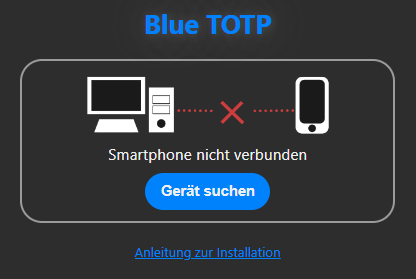
\includegraphics[width=0.5\linewidth]{figures/impl/ext_nicht_verbunden.png}
    \caption[Blue TOTP Extension Home Screen]{Blue TOTP Extension Home Screen. Die Extension aktuell mit keinem Smartphone verbunden und zeigt daher auch nicht die Option zur Einrichtung an.}
    \label{fig: blue totp ext screenshot nicht verbunden}
\end{figure}

\begin{figure}[H]
    \centering
    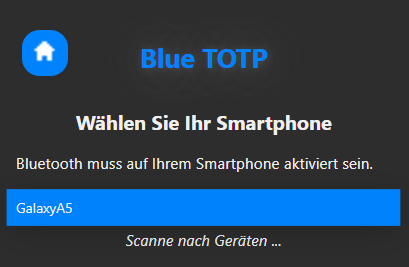
\includegraphics[width=0.5\linewidth]{figures/impl/ext_scan.png}
    \caption[Blue TOTP Extension Scan Screen]{Blue TOTP Extension Scan Screen. Die Extension scannt nach Smartphones mit aktiven Blue TOTP Apps und hat ein Gerät \glqq GalaxyA5\grqq{} gefunden.}
    \label{fig: blue totp ext screenshot scan}
\end{figure}

\begin{figure}[H]
    \centering
    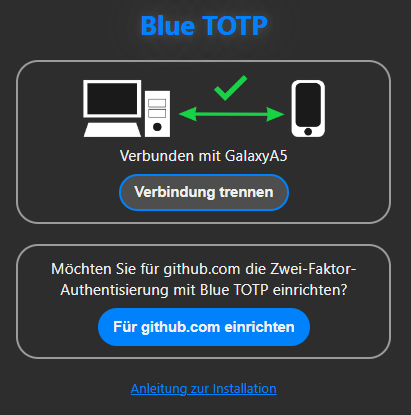
\includegraphics[width=0.5\linewidth]{figures/impl/ext_verbunden.png}
    \caption[Blue TOTP Extension Home Screen (verbunden)]{Blue TOTP Extension Home Screen, der anzeigt, dass die Extension mit dem \glqq GalaxyA5\grqq{} verbunden ist.}
    \label{fig: blue totp ext screenshot verbunden}
\end{figure}

\begin{figure}[H]
    \centering
    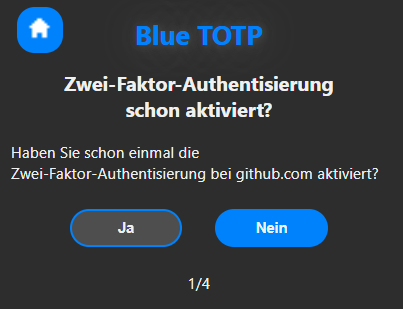
\includegraphics[width=0.5\linewidth]{figures/impl/ext_anleitung_1.png}
    \caption[Blue TOTP Extension Anleitung Screen 1/4]{Blue TOTP Extension Anleitung Screen 1/4. Dieser Screen erfragt, ob der Nutzer bereits die 2FA für die aktuelle Website eingerichtet hat und zeigt dann je nach Antwort eine leicht geänderte Anleitung auf Screen 2/4.}
    \label{fig: blue totp ext screenshot anleitung 1}
\end{figure}

\begin{figure}[H]
    \centering
    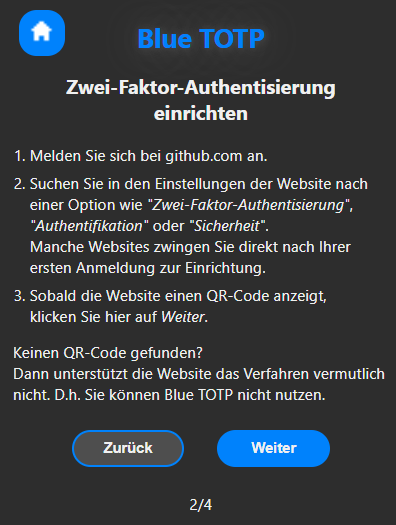
\includegraphics[width=0.5\linewidth]{figures/impl/ext_anleitung_2.png}
    \caption[Blue TOTP Extension Anleitung Screen 2/4]{Blue TOTP Extension Anleitung Screen 2/4. Dieser Screen erklärt dem Nutzer wie er zur 2FA-Einrichtung gelangt. Ziel ist es, dass die Website dem Nutzer den QR-Code anzeigt.}
    \label{fig: blue totp ext screenshot anleitung 2}
\end{figure}

\begin{figure}[H]
    \centering
    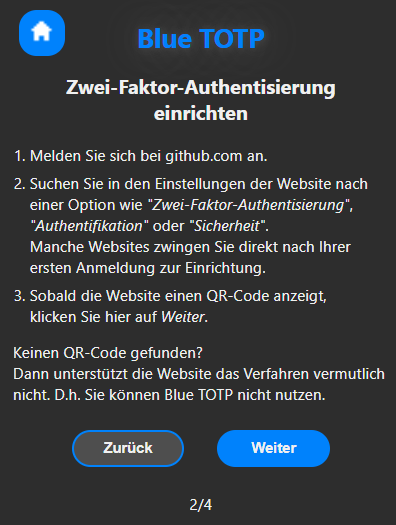
\includegraphics[width=0.5\linewidth]{figures/impl/ext_anleitung_2.png}
    \caption[Blue TOTP Extension Anleitung Screen 3/4]{Blue TOTP Extension Anleitung Screen 3/4. Dieser Screen erfragt den Nutzernamen. Das Eingabefeld ist vorausgefüllt, wenn die Extension den Benutzernamen beim Login mitlesen konnte.}
    \label{fig: blue totp ext screenshot anleitung 3}
\end{figure}

\begin{figure}[H]
    \centering
    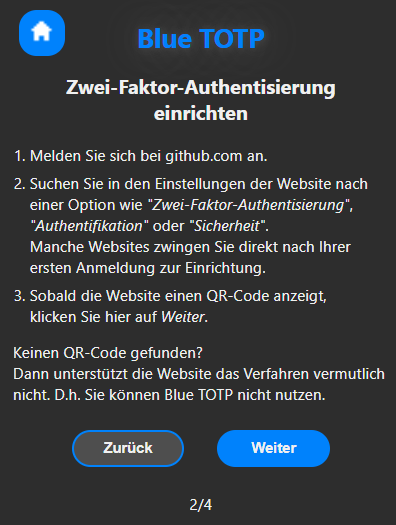
\includegraphics[width=0.5\linewidth]{figures/impl/ext_anleitung_2.png}
    \caption[Blue TOTP Extension Anleitung Screen 4/4]{Blue TOTP Extension Anleitung Screen 4/4. Dieser Screen sagt dem Nutzer, dass er nun mit der Blue TOTP App den QR-Code scannen soll.}
    \label{fig: blue totp ext screenshot anleitung 4}
\end{figure}

\begin{figure}[H]
    \centering
    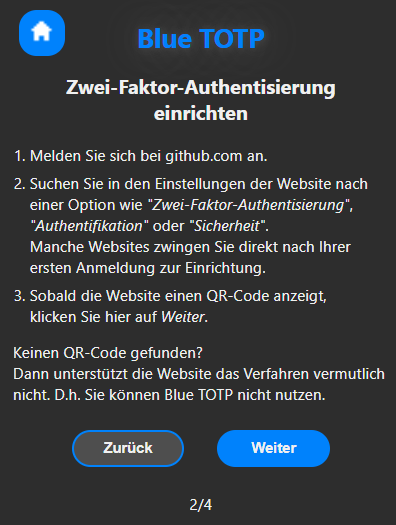
\includegraphics[width=0.5\linewidth]{figures/impl/ext_anleitung_2.png}
    \caption[Blue TOTP Extension Hinweis in Website]{Blue TOTP Extension Hinweis in der Website, der erscheint, wenn der Nutzer das TOTP eingeben muss. Der grün umrandete Bereich ist Ende des TOTP-Eingabeelements. }
    \label{fig: blue totp ext hinweis}
\end{figure}
\newpage
\newpage
    \section{Materialien der Studie}
    \subsection{Interview zur Einrichtung des neuen Verfahrens für zeitbasierte Einmalpasswörter}
\label{anh: interview einrichtung}

\begin{enumerate}
    \item Inwiefern haben Sie die Einrichtung als komplex oder leicht verständlich empfunden?
    \item Wie klar waren die einzelnen Schritte der Einrichtungen? An welchen Stellen wussten Sie nicht, was als nächstes zu tun war und wieso?
    \item Haben Sie (weitere) Anmerkungen oder Änderungsvorschläge für den gesamten Einrichtungsprozess?
\end{enumerate}
Vergleichen Sie die eben durchgeführte Einrichtung (Blue TOTP) mit der traditionellen Einrichtung.
\begin{enumerate}
    \setcounter{enumi}{3}
    \item Wie empfinden Sie den Mehraufwand bei Blue TOTP?
    \begin{enumerate}
        \item Was wären Gründe, Blue TOTP nicht zu nutzen? Wäre der Mehraufwand einer davon?
    \end{enumerate}
    \item Hätten Sie außerhalb der Studie die Einrichtung abgebrochen?
    \item Wie beurteilen Sie die Schwierigkeit der Einrichtung mit beiden Systemen? Fällt Ihnen die Einrichtung mit einem der Systeme leichter oder schwerer? Und inwiefern?
    \item Trauen Sie sich zu, einer anderen Person bei der \textbf{traditionellen} Einrichtung behilflich zu sein?
    \item Trauen Sie sich zu, einer anderen Person bei der Einrichtung von \textbf{Blue TOTP} behilflich zu sein?
    \item Im Vergleich zur traditionellen Einrichtung: Inwiefern wirkt Blue TOTP auf Sie authentisch, als wäre es ein fester Bestandteil der Einrichtung, oder aufgesetzt, als wäre es zusätzlich an die Einrichtung \glqq angebaut\grqq{}?
    \item Haben Sie noch weitere Anmerkungen zum Vergleich zwischen der traditionellen Einrichtung und der Einrichtung mit Blue TOTP?
\end{enumerate}

\subsection{Interview zur Authentisierung mit dem neuen Verfahren für zeitbasierte Einmalpasswörter}
\label{anh: interview authentisierung}

\begin{enumerate}
    \item Sie hatten für 6 Tage die Aufgabe, sich auf der Website anzumelden und eine simulierte Überweisung zu tätigen. Wie ist es Ihnen bei der Nutzung von Blue TOTP ergangen? Hat Ihnen etwas gefallen oder hat Sie etwas gestört?
    \begin{itemize}
        \item Falls negativ:
        Warum hat Sie XY gestört und würden Sie deswegen  Blue TOTP nicht verwenden?
        \item Was müsste geändert werden, damit Sie Blue TOTP gerne nutzen?
    \end{itemize}
    \item Haben Sie sich (weitere) Probleme notiert, die während der Studie aufgetreten sind?
    \item Wie waren Sie vor der Studie gegenüber 2FA eingestellt? Hat die Nutzung von Blue TOTP Ihre Einstellung gegenüber 2FA verändert (und wie)?
    \item Stellen Sie sich vor, Sie können (freiwillig) bei einem Dienst 2FA nutzen. Inwiefern wären Sie dazu bereit, die 2FA mithilfe von Blue TOTP zu nutzen?
    \item Stellen Sie sich vor, Sie müssen bei einem Dienst 2FA nutzen. Z.B. fordert Sie Ihr Arbeitgeber oder der Dienst selbst dazu auf. Inwiefern würden Sie diese Forderung akzeptieren, wenn Sie Blue TOTP dabei verwenden könnten?
    \item Das Ziel von Blue TOTP ist die 2FA mit zeitbasierten Einmalpasswörtern schneller und nutzerfreundlicher zu gestalten. Hatten Sie den Eindruck, dass das Blue TOTP beim Login langsamer oder schneller ist als das traditionelle Verfahren (und inwiefern)?
    \item \textit{Kurz erklären das Blue TOTP gewissermaßen einen Schutz gegen Phishing bietet (auf Phishing-Website sendet Blue TOTP keine Benachrichtigung, da es die Domain der Phishing-Website nicht kennt und so kein TOTP generieren kann).}\\
    Welche Eigenschaft ist für Sie am wichtigsten: die erweiterte Sicherheit, die Nutzerfreundlichkeit sowie schnellere Handhabung oder keins davon?
    \item Wie sehen Sie bei Blue TOTP das Verhältnis aus Aufwand und Nutzen zwischen der Einrichtung und der eigentlichen Nutzung beim Login?
    \begin{enumerate}
        \item Evtl. nachhaken: Überwiegt der Nutzen beim Login (schneller, nutzerfreundlicher) dem Mehraufwand bei der Einrichtung
    \end{enumerate}
    \item In welcher Reihenfolge sind Sie vorgegangen, wenn Sie sich anmelden und authentisieren mussten? (Bsp. erst  App geöffnet, dann Ext. mit App verbunden, dann Login auf Website, …)
    \item Die Blue TOTP App läuft im Hintergrund weiter, auch wenn Sie sie schließen (im Task Manager wegwischen). Haben Sie das wahrgenommen? Wodurch?
    \item Man kann diesen Hintergrundprozess von Blue TOTP auch beenden (Task Manager, Vordergrund Dienste, Blue TOTP, Stoppen). Wie oft haben Sie den Hintergrundprozess beendet und (ggf.) wieso?
    \item Hat die Verbindung zwischen der Android-App und der Browser-Extension einwandfrei funktioniert oder gab es zwischenzeitlich Probleme?
    \item Was ist der übliche Status der Bluetooth-Funktion Ihres \textbf{Computers}? (meist angeschaltet, nur angeschaltet, wenn gebraucht) Und hat die Nutzung von Blue TOTP dieses Verhalten geändert?
    \item Was ist der übliche Status der Bluetooth-Funktion Ihres \textbf{Smartphones}? (meist angeschaltet, nur angeschaltet, wenn gebraucht) Und hat die Nutzung von Blue TOTP dieses Verhalten geändert?
    \item Hat sich Ihrer Wahrnehmung nach der Akku Ihres Smartphones während der 6 tägigen Nutzungsphase schneller entladen als gewöhnlich?
    \item Welches Verfahren würden Sie bevorzugt nutzen, das traditionelle oder Blue TOTP? Warum?
    \item Wo sehen Sie noch Vor- oder Nachteile in Blue TOTP?
    \item Haben Sie weitere Anmerkungen oder Änderungsvorschläge für Blue TOTP?
\end{enumerate}
\newpage
\section{Ergebnisse der Studie}
    \subsection{Tabellen zur Einrichtung von Blue TOTP}
\label{anh: studie ergebnisse setup}

\begin{table}
    \centering
    \begin{center}
    \begin{tabular}{| l | l | l | l | l |}
        \hline
        \textbf{Q1} & \textbf{Median} & \textbf{Mittelwert} & \textbf{Q3} & \textbf{Std.-Abw.} \\
        \hline
        156~s & 177~s & 228~s & 333~s & 104~s \\  
        \hline
    \end{tabular}
    \end{center}
    \caption[Statistische Größen der Einrichtungszeit von Blue TOTP]{Statistische Größen der Einrichtungszeit von Blue TOTP}
    \label{tab: studie setup time}
\end{table}

\begin{table}
    \centering
    \begin{center}
    \begin{tabular}{| l | c |}
        \hline
        \textbf{Gegensatzpaar} & \textbf{Mittelwert} \\
        \hline
        erfreulich / unerfreulich & 1,1 \\  
        \hline
        verständlich / unverständlich & 1,1 \\
        \hline
        kreativ / phantasielos & 1,1 \\
        \hline
        leicht zu lernen / schwer zu lernen & 1,8 \\
        \hline
        wertvoll / minderwertig & 1,5 \\
        \hline
        spannend / langweilig & 0,2 \\
        \hline
        interessant / uninteressant & 1,2 \\
        \hline
        voraussagbar / unberechenbar & 0,7 \\
        \hline
        schnell / langsam & 1,5 \\
        \hline
        originell / konventionell & 1,0 \\
        \hline
        unterstützend / behindernd & 2,1 \\
        \hline
        gut / schlecht & 1,7 \\
        \hline
        einfach / kompliziert & 0,6 \\
        \hline
        anziehend / abstoßend & 0,2 \\
        \hline
        neuartig / herkömmlich & 1,0 \\
        \hline
        angenehm / unangenehm & 1,1 \\
        \hline
        sicher / unsicher & 1,3 \\
        \hline
        aktivierend / einschläfernd & 1,0 \\
        \hline
        erwartungskonform / nicht erwartungskonform & 0,9 \\
        \hline
        effizient / ineffizient & 1,2 \\
        \hline
        übersichtlich / verwirrend & 0,9 \\
        \hline
        pragmatisch / unpragmatisch & 1,6 \\
        \hline
        aufgeräumt / überladen & 2,0 \\
        \hline
        attraktiv / unattraktiv & 0,5 \\
        \hline
        sympathisch / unsympathisch & 0,4 \\
        \hline
        innovativ / konservativ & 1,5 \\
        \hline
    \end{tabular}
    \end{center}
    \caption[Mittelwerte der Gegensatzpaare (UEQ) zur Einrichtung von Blue TOTP]{Mittelwerte der einzelnen Gegensatzpaare (UEQ) zur Einrichtung von Blue TOTP. Werte größer 0 deuten zu den positiven Begriffen (links), Werte kleiner 0 deuten zu den negativen Begriffen (rechts)}
    \label{tab: studie setup ueq item means}
\end{table}
\newpage
\subsection{Tabellen zur Authentisierung mit Blue TOTP}
\label{anh: studie ergebnisse auth}

\begin{table}
    \centering
    \begin{center}
    \begin{tabular}{| l | l | l | l | l || l | l |}
        \hline
        \textbf{Q1} & \textbf{Median} & \textbf{Mittelwert $\bar{x}$} & \textbf{Q3} & \textbf{Std.-Abw.} & \textbf{$\bar{x}$ (IQR)*} & \textbf{$\bar{x}$ ($2\cdot$ STD)*} \\
        \hline
        $5{,}5~s$ & $8{,}5~s$ & $15{,}9~s$ & $15{,}8~s$ & $20{,}8~s$ & $10{,}1~s$ & $11{,}8~s$ \\  
        \hline
    \end{tabular}
    \end{center}
    \caption[Statistische Größen der Authentisierungszeit von Blue TOTP]{Statistische Größen der Authentisierungszeit von Blue TOTP. *bereinigte Daten nach dem Verfahren $1{,}5$-facher Interquartilsabstand (IQR) bzw. $2$-facher Standardabweichung (STD)}
    \label{tab: studie ergebnisse auth time}
\end{table}

\begin{table}
    \centering
    \begin{center}
    \begin{tabular}{| l | l | l | l | l |}
        \hline
        \textbf{Korr.-Koeff. $r$} & \textbf{Freiheitsgrade} & \textbf{$p$-Wert $\bar{x}$} & \textbf{Konf.-Intervall $95\%$} & \textbf{Power}\\
        \hline
        $-0{,}1634$ & $48$ & $0{,}2569$ & $[-0{,}42, 0{,}12]$ & $0{,}2068$ \\  
        \hline
    \end{tabular}
    \end{center}
    \caption[Repeated Measures Correlation zur Authentisierungszeit]{Repeated Measures Correlation zwischen Authentisierungszeit und Tag der Nutzungsphase pro Proband}
    \label{tab: studie ergebnisse auth time rmcorr}
\end{table}    

\end{document}